\documentclass[12pt,hyphens]{report}

% --- PACKAGES ---
%\usepackage[utf8]{inputenc}
\usepackage{graphicx}
\usepackage{caption}
\usepackage[a4paper, margin=2cm]{geometry}
\usepackage{setspace}
\usepackage{titlesec}
\usepackage[most]{tcolorbox}
\usepackage{tocloft}
\usepackage{hyperref}
\usepackage{lscape}
\usepackage{subcaption}
\usepackage{forest}
\usepackage{mfirstuc}
\usepackage{url}
%\usepackage{subcaption}
\usepackage{float}
\usepackage{ifthen}
\usepackage[backend=biber,style=apa]{biblatex}
\addbibresource{chapters/references.bib}
\usepackage{indentfirst} 
\usepackage[none]{hyphenat}
\usepackage{tikz}
\usetikzlibrary{shapes.geometric, arrows.meta, positioning}
\tikzstyle{process} = [rectangle, rounded corners, minimum width=3.5cm, minimum height=1.2cm, text centered, draw=black, fill=gray!10]
\tikzstyle{arrow} = [thick,->,>=stealth]

% --- CUSTOM FORMATTING ---
\setlength{\parindent}{1.5em}  % Paragraph indent
\setlength{\parskip}{0pt}      % No space between paragraphs
\onehalfspacing                % Line spacing
\setlength{\emergencystretch}{2em}

% Remove all default numbering
\renewcommand{\thesection}{}
\renewcommand{\thesubsection}{}
\renewcommand{\thechapter}{}

% Optional: Format unnumbered section titles like chapters (bigger font)
\titleformat{\section}[block]{\normalfont\Large\bfseries}{\thesection}{1em}{}
\titleformat{\subsection}[block]{\normalfont\large\bfseries}{\thesubsection}{1em}{}

% --- DOCUMENT START ---
\begin{document}

% --- FRONT MATTER ---
\begin{titlepage}
    \centering
    % Image at the top
    \includegraphics[width=10cm]{figures/paper_figures/tcd-logo.png}\par
    \vspace{1cm}

    % Department and School
    {\large Department of Political Science\par}

    \vspace{2.5cm}

    % Title section
    {\LARGE\bfseries Forecasting Reliability:\par}
    \vspace{0.3cm}
    {\Large\bfseries LUAS Performance Across Crisis and Recovery\par}

    \vspace{3cm}

    % Name
    {\Large Athena Rodrigues\par}

    \vspace{1.5cm}

    % Supervisor and date
    {\large Supervisor: Dr. Jian Cao\par}
    \vspace{0.5cm}
    {\large August 2025\par}

    \vspace{2cm}

    % Submission information
    {\large Submitted in partial fulfilment of the requirements for the award of the degree\par}
    \vspace{0.3cm}
    {\large Master of Science (MSc) in Applied Social Data Science\par}
    \vspace{0.3cm}
    {\large Trinity College Dublin\par}
\end{titlepage}

\clearpage
\thispagestyle{plain}


\section*{Abstract}

This study investigates the operational reliability of the LUAS light rail network in Dublin by reconstructing tram journeys from public Automatic Vehicle Location System (AVLS) forecast data. Using a custom methodology developed for a data-constrained environment, it analyses three core performance metrics across four pandemic-defined phases from 2020 to 2022: headway regularity, travel time volatility, and journey duration. The findings indicate that while central sections of the LUAS corridors displayed relative stability, peripheral zones and outbound services suffered from extended headways, inconsistent timing, and spatial imbalance; many of which persisted even after restrictions were lifted.

Methodologically, the study demonstrates that forecast data can be systematically reconstructed to infer tram trajectories and diagnose network-level irregularities without requiring proprietary or per-unit records. These findings offer both practical and conceptual contributions: showing how open data can support evidence-based planning and illustrating the structural limitations of frequency-based service models when reliability is unevenly distributed. By mapping the patterns of dependability visible under constrained conditions, the research underscores the importance of equity, adaptability, and transparency in the evaluation of transport performance. It presents a scalable and replicable framework for identifying operational inconsistencies and calls for more responsive planning tools that integrate technical monitoring with everyday service realities.

\clearpage
\thispagestyle{plain}

\section*{Acknowledgements}

I would like to thank my supervisor, Dr. Jian Cao, for their thoughtful guidance and support throughout this project. Their feedback was invaluable in helping me refine both the scope and the clarity of my work. I also wish to acknowledge the faculty and students of the Applied Social Data Science program at Trinity College Dublin for providing a collaborative and intellectually engaging environment that shaped the development of this dissertation.


I am also grateful to my friends, both here and back home, for their encouragement and steady support over the course of this year. Finally, I would like to thank my parents for their continued belief in me and for the foundation of support that has made this work possible. Their patience and generosity throughout my academic journey have been greatlyy appreciated.

\clearpage


\tableofcontents
\newpage

% --- MAIN CONTENT (unnumbered sections with manual TOC lines) ---
\section*{Introduction}
\addcontentsline{toc}{section}{Introduction}

As urbanisation continues to spread upwards and outwards, stable public transport connections between dense city centres and peripheral areas are essential to support efficient and sustainable mobility. The LUAS (Irish for ‘speed’) light rail system plays a key role in supporting County Dublin’s ongoing urban sprawl and population growth, offering high-capacity travel across two directional routes. However, like many transit systems, the LUAS faces persistent operational challenges such as peak-hour bunching, inconsistent tram spacing, and schedule deviations. These issues can reduce service reliability, erode passenger trust, and ultimately deter regular ridership. This study evaluates the reliability of LUAS services between 2020 and 2022 by reconstructing tram journeys from historical forecast data and deriving operational performance metrics. In doing so, this research aims to determine whether widely accepted transit indicators can be extracted from publicly available data, and, if so, how they capture real-world service consistency and stability.

Good service reliability is often perceived as a measure of network quality; when absent, it contributes to increased passenger wait-time anxiety and overcrowding. Using Automatic Vehicle Location System (AVLS) data, this study relies on predicted tram movement to understand the performance of the LUAS infrastructure through an unprecedented stress test, the COVID-19 pandemic. This temporal scope provides a natural division of data into four distinct phases to evaluate changes in public transport. Defined as pre-COVID, lockdown, recovery, and post-COVID, the four phases represent a unique operational context that is shaped by changing demand, altered service patterns, and evolving public health restrictions. By comparing key transit reliability metrics such as headway regularity, travel time volatility, and journey duration across these intervals, the system’s adaptability to fluctuating pressures can be investigated. Together, these provide a multifaceted view of performance, capturing both internal and passenger-perceived reliability. The combined analytical approach enables a comprehensive evaluation of the network’s ability to maintain dependable service under rapidly shifting constraints.

As a relatively modern light rail system with limited publicly data, Dublin's LUAS offers a rare opportunity to assess whether meaningful operational insights can be drawn from forecast data alone. This research assesses the possibility of reliably inferring transit metrics from created journeys, providing insight into operational behaviour under conditions of system-wide disruption. As a result, this study contributes to demonstrating the effectiveness and transparency of rule-based approaches for transport analysis using forecast-only data.

\section*{Literature Review}
\addcontentsline{toc}{section}{Literature Review}

    Framing transit reliability in high-frequency systems requires both conceptual insight and methodological adaptability. This study builds on established strands of research, drawing from prior work on behavioural metrics, the use of real-time prediction data as a proxy for operational performance, and evolving understandings of how public transport systems responded to the pressures of the COVID-19 pandemic. Together, these foundations shape both the methodological choices and the interpretive lens through which the LUAS is assessed.

\phantomsection
\subsection*{Operational Metrics for Transit Service Reliability}
\addcontentsline{toc}{subsection}{Operational Metrics for Transit Service Reliability}

    Service reliability in public transportation refers not only to a vehicle’s ability to arrive ‘on time’ according to schedule but, more importantly, to the system’s ability to maintain consistent and predictable activity. Typically assessed using performance indicators that reflect operations and passenger experience,  this review focuses on three core metrics for analysis: headway regularity, travel time volatility, and journey duration. Each of these captures distinct but interconnected aspects of reliability, which are widely cited as essential for evaluating the transit efficacy.

    Consistently highlighted as a crucial factor in influencing overall performance and reliability in transit research, headways are the time interval between two consecutive vehicles operating on the same route in the same direction \parencite{abkowitz1978transit}. In high-frequency transit systems, where passengers rely less on scheduled timetables and more on the expectation of consistent vehicle spacing, headway regularity offers a more meaningful measure of service quality than traditional punctuality methods. Unlike schedule adherence, which compares vehicle arrivals against a fixed timetable, headway regularity reflects how evenly spaced vehicles are over time, directly influencing passenger wait times and system fluidity \parencite{albright2012transit}.  Prior research supports the use of inferred headways from AVLS data as a reliable foundation for evaluating performance in such contexts. For example, \textcite{furth2007optimal} argue that metrics such as headway deviation and excess waiting time offer a more accurate reflection of passenger experience than on-time statistics. This approach is further supported by \textcite{ma2014measuring}, who highlight the value of AVLS for identifying and correcting irregular service patterns in real time. As such, headway regularity is incorporated as a prime indicator to assess consistent spacing across the LUAS network.

    While headway regularity captures vehicle spacing, it does not account for variation in trip length. Accordingly, \textcite{vanoort2011service} emphasises the importance of capturing multiple dimensions in quick-turnaround operations, especially relating to variability in both arrival patterns and travel timings. To capture this different, yet equally important dimension of service reliability, travel time volatility (TTV) measures the inconsistency in the duration it takes for a transit vehicle to complete a given route, encompassing operational instabilities from unobserved factors such as congestion, signal delays, and varying dwell times. Scholars argue that even these minor unpredictabilities can undermine trustworthiness and reduce passenger confidence, especially in transit where frequency replaces stretch scheduling as the basis for reliability, as seen in the LUAS system \parencite{tirachini2022headway}. From a rider’s perspective, predictability is often more important than strict adherence to timetables, with studies consistently showing that passengers are more sensitive to TTV on arrival than to minor delays. \textcite{benezech2013value} describe this effect as a ‘hidden waiting time’ where unpredictable journey durations create a perception of lost time, even if vehicles are not technically late in reaching the station. Their findings suggest that consistency is often valued more highly than speed in frequent-route networks. Similarly, \textcite{diab2012understanding} demonstrate that even slight improvements in perceived regularity can result in significant gains in rider satisfaction. Accordingly, this study uses travel time volatility to capture short-term fluctuations in duration and service inconsistencies that traditional schedule-based metrics may overlook. 

    Journey duration offers a system-level perspective on reliability not captured by headway regularity or TTV,  that remains meaningful even in the context of segmented passenger journeys. As a key indicator, journey duration refers to the total time required for a vehicle to complete a full trip from origin to destination. It can be evaluated through various methods, including average travel times as well as buffer and planning indices, which aim to capture the contingency passengers required to be considered ‘on time’ \parencite{ma2014measuring}. Other studies have used AVLS to reconstruct full trips and assess reliability by combining in-vehicle travel duration with waiting time, as shown by \textcite{zhang2022prediction} in their evaluation of end-to-end trip consistency. Collectively, this literature supports the inclusion of journey duration as a critical complement to spacing- and variability-based metrics, offering a fuller representation of passenger experience across entire routes.

    These three measures form the analytical backbone of this study, providing a multidimensional framework through which LUAS reliability is assessed from a technical and user experience standpoint. They allow for the identification of spatial and temporal patterns where service performance may deviate from expectations, aligning with passenger perceptions of unreliability. As proxies for quality, they support a behaviourally informed approach to understanding how operational irregularities are experienced at ground level.

\phantomsection
\subsection*{Forecast Data as a Proxy for Observed Transit Performance}
\addcontentsline{toc}{subsection}{Forecast Data as a Proxy for Observed Transit Performance}

    A common limitation in evaluating transit is the lack of access to continuous, stop-level records of actual vehicle arrivals. In contexts where observed arrival data is unavailable, predicted arrival times derived from real-time feeds offer a viable alternative for approximating vehicle behaviour. Inferred changes and disappearances in forecast data, such as fluctuations in predicted arrival times or removal of upcoming trams, have been used in transit research to approximate real tram events like arrivals and departures. Treated as an evolving data stream, these structured forecast patterns allow researchers to reconstruct vehicle trajectories and evaluate network performance in contexts where observed data is unavailable \parencites{sun2016smart}{muller2001trip}. These techniques establish the validity of using inferred events for performance analysis when direct observation is not possible, particularly in regular-interval services where dwell variability and small spacing shifts can disproportionately affect perceived reliability.

    These principles are applied by using time-stamped LUAS forecast snapshots, collected systematically via the public-facing Application Programming Interface (API). Although real-time predictions are published continuously, no archival mechanism exists, necessitating custom logging at consistent intervals. Forecast disappearances are then aligned with structured stop templates and filtered by line and direction to reconstruct tram journey sequences. The method enables consistent identification of stop-level events and spacing patterns without relying on direct arrival observations. \textcite{xu2017arrival} show that prediction accuracy varies systematically with time of day and network load, underscoring the importance of temporal sampling in reliability analysis. This data-driven reconstruction process aligns with broader trends in transit research that leverage real-time feeds to monitor and evaluate system performance, particularly in limited environments. Capturing the evolution of predictions across time supports the extraction of dynamic features that are difficult to observe through static scheduled data.

    Beyond the stop level, this study employs route-aligned identifiers to stitch sequences of inferred arrivals into full tram trajectories. These are then grouped and categorised by pandemic phase, period, direction, and line. This spatial extension allows for TTV and journey duration to be calculated not just at single nodes, but over entire segments or full-line runs. Segment-level analysis has been shown to more accurately reflect the experience of riders, especially in urban transit where issues may cluster in specific zones due to junctions, signal delays, or boarding variability \parencite{zuniga2021estimation}. This approach aligns with broader methodological frameworks that recommend spatially distributed inference to analyse rider exposure to disruption, headway instability, and system resilience \parencite{cats2016risk}. Importantly, these network-wide metrics can be disaggregated by peak periods or pandemic phases, enabling both station-specific and system-level assessments of the LUAS.

    Snapshot-based inference fills a methodological gap by providing a replicable and scalable means of reconstructing service activity using only forecast data. In the absence of direct logs, this approach still supports robust evaluation of core reliability metrics while reflecting a broader shift in transport research toward high-frequency, behaviourally relevant indicators grounded in AVLS data \parencite{tirachini2022headway}. By applying this technique to the LUAS, this study provides a practical and replicable methodology for evaluating system consistency under real-world constraints and offers insight into how public APIs can be utilised to build datasets where direct operational information is withheld.

    Together, these methods validate the use of forecast-based inference as a robust substitute for direct operational data in assessing reliability. By recreating tram behaviour from prediction snapshots, this study can evaluate system performance across both spatial and temporal dimensions, even in the absence of observed arrival logs. The approach not only reflects emerging practices in transit analytics but also ensures that the indicators used are grounded in observable, replicable studies, providing a scalable foundation to analyse network consistency while offering a meaningful way to assess passenger-facing performance within data-constrained environments. While elements of these techniques have been applied elsewhere, this study is among the first to adapt them specifically to Dublin’s LUAS system, demonstrating how fragmented forecast streams can be recombined to evaluate reliability in a previously unexamined context.



\phantomsection
\subsection*{Pandemic Impacts on Transit Behaviour and Reliability}
\addcontentsline{toc}{subsection}{Pandemic Impacts on Transit Behaviour and Reliability}

    The COVID-19 pandemic caused an unprecedented shock to all aspects of daily life, rapidly disrupting public transportation worldwide. Demand patterns, rider behaviour, and service frequency shifted almost overnight, placing strain on transit infrastructure that attempted to maintain operational reliability amid evolving government safety regulations. Observed through historical forecast data, this time serves as a natural stress test for the LUAS network’s adaptability and resilience, with core themes such as passenger trust and stability emerging as central in the evaluation of the impact of pandemic-induced disruption on urban mobility systems \parencite{benita2021human}.

    Traditional approaches of transit research relying on stable demand assumptions, fixed schedules, or long-term averages became inadequate for understanding system performance under these changing conditions. As a result, studies called for data-driven frameworks that could measure real-time adaptability and assess how infrastructure respond to external shocks \parencite{gutierrez2021covid}; or focused on examining how operational trade-offs during lockdowns, such as reduced service levels, affected long-term reliability and rider trust \parencite{deborger2021covid}. Researchers also turned to higher-frequency data and temporal segmentation techniques to better understand system behaviour during lockdowns and reopenings. Rather than treating the pandemic as an outlier, it was positioned as a critical opportunity to examine structural weaknesses and the limits of network flexibility. Collectively, this body of work has expanded the analytical lens through which transit performance is evaluated, encouraging more responsive and situationally-aware approaches.

    In the Irish context, COVID-19 significantly altered public travel behaviour and usage, with a steep nationwide decline in ridership that raised concerns about long-term behavioural shifts away from transit due to safety and comfort anxieties \parencite{hynes2020utility}. During partial reopening phases in Dublin, many remained hesitant to resume the use of transit such as the LUAS, especially in densely populated corridors, highlighting issues of accessibility and behavioural adaptation across different demographic and geographic contexts \parencite{caulfield2021trinity}. Meanwhile, \textcite{marra2022impact} provide longitudinal evidence of pandemic-driven changes in travel timing, route preferences, and transfer patterns, all of which suggest significant disruption to previously stable urban mobility norms. These findings contribute to a localised understanding of how the pandemic impacted operations, rider confidence, and overall transit use.

    Both international and Ireland-specific research supports the segmentation of data into pandemic-related phases for comparative analysis. These studies justify the use of historical forecast data to examine service regularity, inferred arrival patterns, and volatility under conditions of external stress. However, few have combined multiple internal reliability metrics to evaluate system performance during this period, limiting a more holistic understanding of how different dimensions of service consistency evolved under pandemic conditions. In the context of LUAS, this approach allows for a deeper understanding of how reliability shifted in response to fluctuating demand, constrained operations, and evolving public confidence—factors essential to interpreting performance in a time defined by uncertainty.


\section*{Data and Processing}
\addcontentsline{toc}{section}{Data and Processing}

\phantomsection
\subsection*{Data Source and Structure}
\addcontentsline{toc}{subsection}{Data Source and Structure}

    Operated under the oversight of Transport for Ireland (TFI), LUAS real-time tram arrival information is published through an API that sources data from real-time AVLS updates. While this program is accessible via data.gov.ie, historical records are not publicly archived or easily available on request. Directly scraping these logs was not feasible due to the time and computing constraints of this project. Instead, this study makes use of an independently archived dataset compiled by Dublin-based developer Eoin O’Brien, who has collected continuous forecast logs from the API referenced above, spanning January 2020 to October 2022 \parencite{obrien2022historical}. When contacted, and on his website, O’Brien mentioned no restrictions on academic use and expressed support for its inclusion in this study. Furthermore, as only publicly available, non-identifiable AVLS data is used, no personal or private information was accessed, meeting ethical requirements.

    This dataset contains timestamped forecast records of all upcoming tram arrivals, logged approximately every two minutes, across all LUAS stations and lines. In total, it comprises over 160 million rows, providing a comprehensive view of the system’s behaviour over time. Given the size and regularity of logging, records were processed into time-based \texttt{ServiceDay} groupings to enable scalable batch processing, more efficient validation, and robust temporal analysis. This field also ensured complete journeys, as the operational schedule runs from around 5:30 am to 12:30 am, ensuring the inclusion of trams running past midnight, into the following calendar day \parencite{tfi_luas}. Additional processing was performed to extract time-of-day categories: morning, midday, evening, and night.

    The key columns extracted and used for reconstruction and analysis were:

\begin{itemize}
  \item \texttt{DateTime}: the timestamp of the forecast; standardised via \texttt{timedelta}
  \item \texttt{Origin}: the station at which the forecast was recorded; renamed \texttt{Stop} for clarity
  \item \texttt{Line}: the major route of the station; \texttt{Red} or \texttt{Green}
  \item \texttt{Direction}: the tram trajectory; \texttt{Inbound} (North/East) or \texttt{Outbound} (South/West)
  \item \texttt{Minutes}: the number of minutes forecasted until arrival at the stop
  \item \texttt{Destination}: the scheduled end terminus of the tram
  \item \texttt{ServiceDay}: the operational date of the service taken from \texttt{DateTime}
  \item \texttt{Period}: the time of day the forecast occurs, calculated from \texttt{DateTime}
\end{itemize}

\phantomsection
\subsection*{Pandemic Phase Segmentation}
\addcontentsline{toc}{subsection}{Pandemic Phase Segmentation}

    A major factor in processing was the need to account for the impact of the COVID-19 pandemic; to reflect how this evolving public health emergency affected operations, the data was segmented into distinct phases based on major policy milestones. Although the Irish Government officially implemented national restrictions on March 27, 2020, under the Health Act 2020, the pre-COVID phase ends slightly ahead of the official lockdown date to account for anticipatory behavioural shifts and early institutional responses \parencites{govireland2020a}{govireland2020b}. Gradual reopening at the end of May 2021 introduced what was widely referred to as the "new normal,” though this phase still involved capacity limits, vaccination certification, and intermittent restrictions \parencite{govireland2021}. The final removal of public health restrictions in January 2022 marked the beginning of a post-pandemic phase of near-normalised operations \parencites{govireland2022}{depthealth2022}.

    Accordingly, the dataset is divided into four phases for comparative analysis:

\begin{itemize}
  \item \textbf{Pre-COVID}: 20 January 2020 to 20 March 2020
  \item \textbf{Lockdown}: 21 March 2020 to 31 May 2021
  \item \textbf{Recovery}: 1 June 2021 to 21 January 2022
  \item \textbf{Post-COVID}: 22 January 2022 to 22 October 2022
\end{itemize}

\phantomsection
\subsection*{Stop Templates}
\addcontentsline{toc}{subsection}{Stop Templates}

\begin{figure}[H]
  \centering
  \includegraphics[width=0.6\textwidth]{figures/paper_figures/station_map.jpg}
  \caption{LUAS Station Routes. Source: Transport for Ireland}
  \label{fig:luas_routes}
\end{figure}

    To facilitate the stitching of full tram journeys, a dictionary of stop templates was created to reflect the sequential order of LUAS stops along each route. These initially mirrored standard full-service patterns for both lines, seen in Figure~\ref{fig:luas_routes}, and served as a reference for identifying valid progressions within the forecast snapshot data. This approach ensured that only plausible directional sequences were linked, helping to reduce errors from route anomalies or forecast noise.

    However, during early exploration, it became clear that some snapshots terminated unexpectedly at intermediate stops, typically Dominick or Connolly; these truncated journeys were not necessarily indicative of data error but reflected real-world operational constraints like city centre disruptions, partial routings, or planned diversions. Rather than discard these cases, the stop templates were expanded to include any recurring endpoints that appeared with sufficient frequency. This adaptive strategy allowed for a more accurate reconstruction of service behaviour by acknowledging that not all trams span the entire route.  Using this approach, over 375,000 valid tram journeys were reconstructed across both lines and directions from January 2020 to October 2022, capturing not just full-route trips but also consistent partial services. The result was a consistent and flexible matching process that captured the actual behaviour of LUAS vehicles, avoiding assumptions about completion while maintaining logical structure.
    
    This study intentionally grounded stop templates solely on destination-based endpoints, rather than attempting to infer full start-to-end routes from partial data. By focusing only on observable destinations, defined by significant stations seen in end destination counts, speculative reconstruction of full routes and potential data overfitting was avoided. The handling of non-traditional terminus journeys was important in capturing irregular or truncated services caused by disruption, without introducing errors from falsely completed journeys. Using destination frequency as a filtering mechanism ensured that the templates remained representative of real operational patterns, further ensuring the building process was tractable and replicable. However, as the approach relies on periodic forecasts rather than continuous tracking, some journeys may be over- or under-segmented, particularly during peak congestion or when data gaps occur between snapshots. Given the nature of forecast data, exact route replication was never expected; instead, the reconstruction prioritised internal consistency and behavioural plausibility over fine-grained precision.



    \phantomsection
\subsection*{Analytical Limitations and Design Decisions}
\addcontentsline{toc}{subsection}{Analytical Limitations and Design Decisions}

    A significant limitation of this study was the absence of unique tram vehicle identifiers in the forecast dataset. Without access to vehicle IDs, it was not possible to definitively track individual trams as they moved through the network; this became particularly challenging in high-frequency segments, where multiple trams might serve the same direction within a short time frame. To address this, trams were reconstructed using sequential station-based inference, guided by forecasted arrival timestamps and directional stop templates, allowing for the approximation of tram movement across the network without overcomplicating the stitching process. Temporal filters helped prevent implausible overlaps, particularly during peak periods, further maintaining the integrity of the inferred journeys even in the absence of direct vehicle tracking. Due to these constraints, the focus of the analysis shifted toward broader route-level dependability rather than specific operations. While this approach restricts the ability to evaluate factors such as inter-trip recovery or tram-specific consistency, it remains aligned with the passenger perspective of reliability, which is primarily shaped by observed spacing, journey duration, and scheduling at the station level.

    A further methodological decision was the exclusion of the Status Message field provided in API logs. Although these messages occasionally offered useful context on disruptions, their lack of standardisation, inconsistent phrasing, and absence of structured metadata limited their analytical value. Incorporating them would have required subjective interpretation or manual parsing, creating potential risks of introducing noise or misclassification. As a result, stops were assumed to be active unless indicated otherwise in the log structure, acknowledging that some inferred journeys may include segments that were operationally bypassed but still could have been logged by the AVLS system. In cases where sequences terminated early or deviated from full-route templates, the data was not treated as erroneous; instead, recurring truncated journeys were accepted as legitimate service patterns, with acknowledgement of partial operations due to diversions, disruptions, or modified timetables. This decision was consistent with the study’s overarching principle of prioritising observed system behaviour over assumed norms. While this may occasionally include non-revenue or non-passenger movements, it ensures that the analysis captures the full scope of operational irregularities rather than smoothing through strict filtering.

    Finally, the high temporal resolution, with forecasts recorded every two minutes, and sheer scale of over 160 million rows introduced inherent limitations for capturing stop-level events with exact precision. Some arrivals or departures may have occurred between snapshot intervals, potentially leading to under- or over-representation of certain events. However, given the volume and consistency of the logs, averaged over varying periods and phases, this granularity was deemed sufficient for identifying broader service patterns and supporting the computation of regularity across the network.
\section*{Methodology}
\addcontentsline{toc}{section}{Methodology}

\phantomsection
\subsection*{Design Development Logic}
\addcontentsline{toc}{subsection}{Design Development Logic}

\begin{figure}[H]
\centering
\begin{tikzpicture}[node distance=2.5cm]

\tikzstyle{process} = [rectangle, rounded corners, minimum width=5.5cm, minimum height=1.6cm, text centered, draw=black, fill=gray!10, align=center]
\tikzstyle{arrow} = [thick,->,>=stealth]

\node (stage1) [process] {
    \begin{minipage}{7cm}
    \centering
    \textbf{Stage 1: Station-Level Forecasts}\\
    Identify valid countdowns from snapshot logs
    \end{minipage}
};
\node (stage2) [process, below of=stage1] {
    \begin{minipage}{7cm}
    \centering
    \textbf{Stage 2: Tram Journey Construction}\\
    Stitch stop-level events into full tram trajectories
    \end{minipage}
};
\node (stage3) [process, below of=stage2] {
    \begin{minipage}{7cm}
    \centering
    \textbf{Stage 3: Metric Calculation}\\
    Compute headway regularity, volatility, and journey duration
    \end{minipage}
};

\draw [arrow] (stage1) -- (stage2);
\draw [arrow] (stage2) -- (stage3);

\end{tikzpicture}
\caption{Three-stage Pipeline}
\label{fig:processing-flowchart}
\end{figure}

    Early attempts to construct LUAS tram journeys directly from raw forecasts aimed to generate both single-stop arrivals and full-route forecasts in one processing step. However, this approach quickly proved unmanageable, due to excessive aggregation, duplicate assignments, and ambiguous mappings, which compromised data clarity and reliability. These issues were especially pronounced around city centre stations, where high service frequency, shared-route stops, and inconsistent directional inference complicated accurate reconstruction. In response to these shortcomings, the construction process was restructured into a multi-stage plan to improve reproducibility and maintain control while ensuring the accurate building of services. A rule-based approach was selected over machine learning or simulation-based alternatives to ensure transparency, interpretability, and full control over how forecasts were translated into operational journeys, as the scale and intricacy of real-world transit activity risk being lost or oversimplified in more abstracted modelling methods.

    Stage one focused on grouping raw forecast logs into coherent station-level tram segments. Stage two then constructed full tram trips by assembling these segments according to predefined stop templates, ensuring directionally valid and physically plausible routes. Stage three applied analytic transformations to the stitched journeys to allow for the computation and visualisation of the performance metrics. This process was refined through staged development, with initial prototypes tested on a single month to validate forecast chunking and route-matching logic before being scaled across the full dataset and pandemic phases. The resulting modular pipeline was designed to handle the large data, concurrent operations, and potential irregularities, enabling a systematic review of service reliability.



\phantomsection
\subsection*{Stage 1: Building Station-Level Forecasts}
\addcontentsline{toc}{subsection}{Stage 1: Building Station-Level Forecasts}

    The first stage of journey reconstruction involved identifying coherent sequences of predicted tram arrivals at individual LUAS stations. Because the dataset contained no unique vehicle identifiers, it was necessary to infer per-tram behaviour through the analysis of arrival prediction evolution. To achieve this, raw forecast logs were first grouped by \texttt{Line}, \texttt{Destination}, \texttt{Station}, and \texttt{ServiceDay}, and then sorted chronologically by the forecast timestamp (\texttt{DateTime}). Each log captured a forecasted number of minutes until a tram’s expected arrival at a station, recorded at roughly two-minute intervals; over time, these snapshots formed countdown sequences that tracked the predicted approach of a tram toward a stop. The function \texttt{stitch\_forecasts\_by\_station()} was developed to extract these sequences by scanning grouped logs for patterns that resembled realistic tram approaches. This process transformed disaggregated forecasts into discrete records, referred to as \texttt{StationJourneys}, each representing the inferred movement of a single tram arrival at a specified station. To isolate valid \texttt{StationJourneys}, the function applied four rule-based constraints: temporal continuity, countdown progression, sequence integrity, and minimum length. Each constraint addressed a key challenge in distinguishing real tram approaches from noise, logging anomalies, or overlapping vehicle forecasts, an essential step in high-frequency urban segments.

    Temporal continuity ensured that logs within a sequence were chronologically valid and associated with the same tram. To do this, entries were only linked if the time difference between consecutive logs was between 0 and 8 minutes. The upper limit prevented the erroneous merging of two separate trams that may have shared a destination and direction but were too far apart in time to plausibly belong to a single trip. The lower limit filtered out redundant duplicates, often caused by AVLS system miscalculations, latency-induced re-logging, or feed errors that recorded multiple timestamps within the same minute. Without this constraint, journeys could be artificially extended or misidentified, particularly in central segments where multiple trams in the same direction may appear within short intervals (peak periods). Along with this, the countdown progression leveraged the expectation that a tram approaching a stop should show a generally decreasing arrival time. Since forecasts were sampled every two minutes, an uninterrupted approach would typically show a two-minute drop between consecutive logs. However, AVLS are prone to short-term prediction noise due to signal delays, recalibration, or passenger boarding variation. To account for this, the function was designed to allow modest fluctuations: up to 2 minutes early (-2) or up to 5 minutes late (+5) between logs. The lower bound reflects a realistic allowance for minor system corrections, such as a tram arriving slightly ahead of forecast. The upper bound was selected based on exploratory testing, which showed that increases of more than 5 minutes were rare and often reflected a new tram entering the feed. These thresholds preserved the expectation of a steady countdown while accommodating real-world inconsistencies, ensuring only credible sequences were retained.

    Sequence integrity maintained logical structure by filtering out errors that could distort the inferred journeys. Repeated timestamps were removed to avoid inflating trip length through duplicated entries. Additionally, a reset condition was implemented to split sequences when a tram appeared to have arrived and was then followed by a new forecast. Specifically, if a log within a sequence showed a minimum prediction of less than or equal to 1 minute, and the following log showed an increase of 3 or more minutes, the sequence was cut at that point, and a new sequence was initiated. This logic handled common edge cases where a tram disappeared from the prediction feed and was rapidly replaced by the next approaching service, frequently seen in high-traffic segments. To further enforce sequence validity, a minimum forecast length ensured each retained log reflected a meaningful observation of tram movement. Sequences were required to contain at least five forecast entries to qualify as valid \texttt{StationJourneys}. This threshold was chosen to balance inclusivity and rigour: short enough to allow for partial journeys or low-frequency periods, but long enough to avoid retaining spurious or fragmentary prediction chains. Including too-short sequences risked misinterpreting random forecast noise as legitimate vehicle movement, which would undermine later network-level stitching.

    Together, these constraints enabled the transformation of raw, forecast data into structured station-level units representing plausible tram arrivals. Although no direct arrival flag exists, the final entry in each sequence is treated as a presumed arrival, inferred through countdown progression and the subsequent disappearance or reset of predictions in the forecast feed. With over 160 million records processed into coherent StationJourney segments, each tagged with a unique StationJourneyID, these sequences formed the foundational building blocks for all later stages of full-line reconstruction. Although the absence of vehicle-level IDs limited exact recreation, this rule-based logic produced reproducible sequences robust enough to support system-level reliability analysis. A sample output of a complete StationJourney is shown below (Figure~\ref{fig:station-level}), illustrating how a forecast countdown is linked from its initial appearance to the presumed arrival.

\begin{figure}[H]
  \centering
  \includegraphics[width=0.6\textwidth]{figures/paper_figures/station_level.png}
  \caption{Station-Level Forecast Segment Example}
  \label{fig:station-level}
\end{figure}

\phantomsection
\subsection*{Stage 2: Constructing Tram Journeys}
\addcontentsline{toc}{subsection}{Stage 2: Constructing Tram Journeys}

    The second stage of this study linked the previously stitched station-level segments into continuous, directionally valid journeys. This process relied on spatial and temporal alignment using predefined stop dictionaries, which served as structural references for identifying plausible combinations of \texttt{StationJourneysIDs} to represent a continuous tram journey. As these templates mirrored the physical order of LUAS stops by line and direction, a consistent matching process without reliance on operator or schedule assumptions was made possible. To implement this process, the \texttt{build\_clean\_tram\_journeys()} function first enriched the station-level logs with an \texttt{EstimatedArrival} variable, calculated by adding the predicted \texttt{Minutes} value to the log’s original timestamp (\texttt{DateTime}). This addition placed all forecasts on a uniform timeline of expected arrivals rather than forecast issuance, enabling a cleaner temporal comparison between stops. Additionally, the \texttt{ServiceDay} field was extracted to restrict stitching to individual operational days and prevent cross-day contamination.

    A lookup table (\texttt{sjid\_info}) was then constructed, containing each \texttt{Station\allowbreak Journey\allowbreak ID}’s station name, direction, estimated arrival time, and service day. This structure supported efficient iterative scanning of potential matches across possible segment combinations during the stitching process. Construction began by identifying a segment corresponding to the first stop in a given template. From this anchor, the function advanced sequentially through the stop order, attempting to append additional segments that matched both the expected stop and direction. To qualify, a candidate’s estimated arrival time had to fall within six minutes of the preceding segment. This temporal threshold approximated the realistic progression of travel times through the LUAS network, tolerating minor timing variations while minimising the risk of linking unrelated vehicles. Although not a strict headway value, the six-minute window served as a practical cutoff for inferring continuity, particularly in areas where tram forecasts often overlap.

    The function allowed for a maximum of one missing stop, improving resilience against forecast gaps or partial sequences and addressing common edge cases where forecasts were truncated or dropped near termini due to AVLS inconsistencies. However, all retained journeys were required to contain at least six matched stops to qualify for inclusion; this threshold ensured that even reduced services reflected genuine vehicle movement. A stricter filter, requiring 15 stops, was later applied during metrics calculation to isolate near-complete journeys suitable for analysis. Furthermore, to prevent duplication and ensure segment uniqueness, each \texttt{StationJourneyID} was assigned to only one \texttt{TramJourney}. Once a segment was successfully matched, it was flagged as used and excluded from subsequent iterations. This safeguard was important in central LUAS segments with shared tracks and overlapping directions, where sequence ambiguity was more likely. Upon completion, each journey was assigned a unique \texttt{TramJourneyID}, constructed from its origin, destination, and service day, with an incremental counter (\texttt{BRO\_SAN03\_2021\_06\_14}), enabling consistent referencing in downstream analysis.

    Although the absence of explicit tram vehicle identifiers limited the ability to track individual units, this approach produced repeatable and interpretable approximations of real-world tram movements. By integrating structured stop templates, estimated arrivals, and conservative temporal thresholds, fragmented station-level logs were reconstructed into coherent, plausible journeys. While some uncertainty remains due to prediction gaps or AVLS anomalies, the resulting dataset is robust enough to support comprehensive reliability evaluation in the next stage.

\phantomsection
\subsection*{Stage 3: Computing Reliability Metrics}
\addcontentsline{toc}{subsection}{Stage 3: Computing Reliability Metrics}

    With tram journeys reconstructed and grouped, the resulting records formed the basis for computing the three key transit metrics: headway regularity, travel time volatility, and journey duration. Due to the uneven durations of the phases, these were averaged and further disaggregated by time of day to capture fluctuations. The \texttt{generate\allowbreak\_final\allowbreak\_segments()} function transformed each \texttt{TramJourneyID} into a sequence of inter-station segments by retaining only the final forecast log for each \texttt{StationJourneyID}, representing the final predicted arrival of a tram at each stop. These arrival logs were kept in stop template order, and station pairs (each log’s Current Station to its Next Station) were linked to calculate \texttt{TravelTimeMinutes}, the inferred duration between two consecutive stops. To illustrate the resulting final segments, Figure~\ref{fig:arrival_journey} presents a single complete tram journey.

\begin{figure}[H]
  \centering
  \includegraphics[width=0.6\textwidth]{figures/paper_figures/arrival_journey.png}
  \caption{Example of an Arrival Journey}
  \label{fig:arrival_journey}
\end{figure}

    Headway regularity was used to assess the consistency of tram arrivals during stages of high demand; these were calculated as the time intervals between two consecutive trams at the same stop, grouped by line and direction to account for overlapping services along shared-direction tracks. For each stop, arrival times were sorted chronologically, and the time difference between successive trams was saved as \texttt{HeadwayMinutes}. These values were then binned into two peak periods, Morning (06:00 to 10:00) and Evening (15:00 to 19:00), to isolate intervals of high passenger demand where service regularity was most critical. To reduce the influence of outlier values caused by disruptions or noise, Interquartile Range (IQR) filtering was applied. The resulting \texttt{AvgHeadwayMinutes} provided a measure of how evenly spaced trams were at each stop, helping to identify locations with irregular service frequency or potential gaps. Inconsistent headways can indicate a need for increased vehicle deployment or operational adjustments to improve line-level reliability and passenger experience.

    Travel time volatility (TTV) was used to quantify the consistency of travel durations between consecutive stops. For each inter-stop segment (Stop → NextStop), the standard deviation of \texttt{TravelTimeMinutes} was calculated and grouped by hour of day. These hourly TTV values were then averaged across the broader periods (Morning, Midday, Evening, and Night) and grouped by line and direction; this breakdown enabled the identification of when and where tram movement was most variable. High volatility values indicated operational instability or external disruptions that affected the predictability of arrival times. By highlighting segments with greater variability, TTV helped reveal structural inefficiencies in the network. This metric can support targeted interventions such as timetable refinements, signal prioritisation, or infrastructure improvements to improve the regularity and predictability of tram movement across specific corridors.

    Journey duration provided a baseline for evaluating overall service efficiency, measuring the total time taken by each reconstructed tram journey from start to end. Rather than using the difference between the first and last arrival timestamps, duration was computed by summing the \texttt{TravelTimeMinutes} values for all inter-stop segments within each \texttt{TramJourneyID}. This method accounted for inconsistent spacing or incomplete countdowns and offered a more reliable reflection of real movement, particularly where arrival predictions were irregular or truncated before reaching zero. Each journey was categorised by its starting hour into time-of-day periods to enable comparative analysis across demand windows. IQR filtering was again applied to remove extreme durations, producing a refined dataset representative of typical service conditions. Trends in journey duration across phases and directions offered insights into broader operations and allowed planners to detect stretches requiring schedule adjustments, address systemic slowdowns, or further look into congestion-prone areas.

    Together, these three measurements offered a comprehensive framework for assessing LUAS service over time, enabling the identification of both spatial and temporal inconsistencies in delivery. The structured outputs supported comparative analysis of operative adaptations to evolving conditions across pandemic phases. Additionally, by incorporating time-of-day breakdowns within each phase, the analysis can capture intra-day variability in performance. These measures ensured that the reconstructed dataset could support robust, reproducible evaluations of network reliability, grounded in established transit research methodologies and responsive to real-world operational dynamics.


\section*{Analysis}
\addcontentsline{toc}{section}{Analysis}

\phantomsection
\subsection*{Overview}
\addcontentsline{toc}{subsection}{Overview}

    While the LUAS network operates in a context where a degree of variability is expected, the benchmarks published by Transport for Ireland (TFI) provide a valuable reference point for assessing operational reliability. This analysis focuses on the previously discussed metrics as each captures a distinct dimension of operational performance and is assessed in line with the four phases, with further disaggregation by time of day to account for both structural and temporal variation in network behaviour. Headway regularity reflects the spacing of stop-level service, TTV captures the variability between stops, and journey duration provides a measure of overall efficiency across full routes. Given the influence of route geometry and stop spacing on standard deviation, visualisations help contextualise and highlight otherwise obscured patterns; in particular, graphical outputs identify spatial asymmetries, directional trends, and clusters of disruption across the network. As no observed arrival logs or vehicle-level identifiers are publicly released by Transport for Ireland, formal validation was not possible; however, internal checks were built into each processing stage to enforce strict matching conditions using stop templates and temporal thresholds. In addition, random spot checks of reconstructed journeys confirmed that inferred trajectories followed plausible timing, directionality, and stop progression. Although each metric is presented independently in the sections that follow, their interrelationships and evolution across pandemic phases are considered collectively to support a broader understanding of network stability.

\phantomsection
\subsection*{Headway Regularity}
\addcontentsline{toc}{subsection}{Headway Regularity}

    Headway regularity reflects the consistency in timing between consecutive tram arrivals at a given stop and is a core determinant of perceived reliability in high-frequency networks. While the LUAS does not operate on a fixed timetable, Transport for Ireland recommends a target headway of 3 to 5 minutes during peak hours as a benchmark for optimal service delivery  \parencite{tii_luas}. This target timing forms a baseline against which operational deviations, bunching, or long waits can be evaluated. Within a transit system like the LUAS, where schedules are implicitly embedded in passenger expectations, irregular headways can have disproportionate effects on crowding, platform dwell times, and overall journey time reliability. These patterns are illustrated in the Appendix section Headway Regularity, which visualises spatial clusters of service volatility across both time and direction. A consistent structural pattern emerges with central segments of both lines reliably maintaining moderate, predictable headways, while outer termini experienced sustained irregularity, notably during evening peaks and outbound travel.

    Morning services were generally more structured, mainly along inner corridors. Across all phases, inbound travel through central stops such as Smithfield, Four Courts, Parnell, and Marlborough maintained average headways below 9 minutes, even during the lockdown. This consistency likely reflects strategic prioritisation of commuter flows into the city core during high-demand hours, where service regularity is both more visible and more operationally consequential. In contrast, outer zones such as Cherrywood, Fortunestown, and Cabra frequently recorded headways over 20 minutes, with only marginal improvement in the post-COVID phase. This suggests enduring gaps in frequency at the edges of the network, where demand may be lower but reliability remains essential for equity of access. The persistence of this disparity across time implies that morning service recovery efforts disproportionately favoured high-demand core areas, potentially at the expense of peripheral users.

    Evening peak headways exhibited more pronounced directional imbalance, highlighted on outbound routes. This asymmetry likely reflects both higher return demand and residual disruption from earlier midday delays, which can propagate across the schedule and accumulate by late afternoon. Trams departing the city towards Saggart, Cherrywood, and Hospital consistently exhibited the longest headways, often surpassing 22 minutes. While inbound trams into the city centre remained relatively stable at 10 to 13 minutes across most phases, outbound frequencies remained fragmented even after official service recovery. This imbalance is particularly consequential during evening peaks when passengers rely on dependable return journeys to suburban or peripheral areas. It also underscores the operational challenges of maintaining bidirectional regularity across an extended network span with finite trams and staffing resources.

    Taken together, these trends reveal a resilient yet spatially uneven service model. The LUAS was able to preserve moderate headway consistency across central corridors, especially for inbound morning travel, reinforcing the network’s functional backbone. However, this stability came at the cost of persistent irregularity and extended gaps at peripheral stops, particularly during evening outbound periods. Importantly, the network’s post-pandemic recovery did little to rebalance this spatial disparity. Instead, it reinforced a hierarchy of regularity, where inner-city predictability was preserved, and outer-zone variability remained structurally embedded. For passengers, especially those living or working beyond central Dublin, this translates to longer effective wait times, increased uncertainty, and a diminished perception of service dependability. These patterns raise critical questions about the equity of resource allocation, the limits of operations in extended networks, and the degree to which transit systems can, and should, sustain balanced service trustworthiness across all user geographies.

\phantomsection
\subsection*{Travel Time Volatility}
\addcontentsline{toc}{subsection}{Travel Time Volatility}

    While headway regularity captures frequency stability at the stop level, travel time volatility reveals the extent to which journey consistency fluctuates along the network’s spatial and directional axes. Travel time volatility (TTV) refers to the variability in travel durations between consecutive tram stops. This is averaged across multiple trips within the various defined timeframes and directions. Maintaining low TTV is essential to sustaining perceived reliability for rapid transit systems. While the TFI does not specify an official threshold, this analysis adopts a one-minute benchmark, indicating that in a system where typical rider trips span short segments, average deviations above one minute reflect meaningful inconsistency. This threshold also provides a practical basis for comparing variability across both densely spaced inner-city stations and more widely distributed peripheral areas. Across the phases, approximately 73 to 78 per cent of stops recorded average TTV below this one-minute threshold, indicating broad but uneven reliability. These findings are supported by line-specific visualisations presented in the Appendix section Travel Time Volatility, which reveal directional and spatial variation not evident in summary statistics. Patterns of volatility were not uniformly distributed, with each line exhibiting distinct spatial and directional characteristics that shaped the overall stability of service.

    On the Green Line, TTV remained relatively low and spatially contained throughout the data duration. During pre-COVID, average volatility stayed below one minute for over three-quarters of stops, with moderate peaks up to 4.28 minutes appearing around core city-centre locations such as Harcourt and Charlemont during peak hours. Lockdown introduced more directional instability, particularly in outbound services south of Sandyford, where extended segment lengths and lower frequencies likely contributed to increased variability. Visualisations show this volatility remained geographically localised, with little evidence of systemic disruption. Recovery and post-COVID phases marked a return to broader consistency; average TTV values stabilised, with 74 per cent of stops remaining below the one-minute threshold during recovery and 73 per cent post-COVID. Small, residual fluctuations persisted in transitional suburban zones, such as Milltown, but no strong directional asymmetries were observed. This consistent pattern suggests that the Green Line adapted well to pandemic-induced shifts in ridership and maintained operational balance throughout.

    In contrast, the Red Line exhibited higher and more spatially dispersed volatility throughout the same phases. The pre-COVID phase, at inner-city segments such as James’s, Abbey Street, and Heuston, recorded moderate TTV levels, often associated with multimodal interfaces and higher passenger turnover. During the lockdown, inbound volatility peaked at Kylemore and Connolly, while outbound variability was dispersed across western zones, including Tallaght, Cookstown, and Suir Road. The Red Line also recorded the highest segment-level TTV overall, reaching 4.94 minutes. Although 75 per cent of stops remained below the one-minute threshold, this reflects the line’s length, stop density, and directional complexity rather than a uniformly reliable experience. Post-lockdown recovery did not significantly reduce this dispersion. Visual analysis of post-COVID maps shows elevated TTV at outer stops such as Hospital and The Point, with central segments maintaining better control. The persistence of directionally imbalanced variability, particularly during evening outbound service, points to underlying constraints in scheduling resilience and corridor complexity, especially where the line intersects with mixed traffic environments or less predictable demand flows.

    These patterns underscore the importance of spatial and directional sensitivity when interpreting TTV within a high-frequency light rail system. While the majority of stops on both lines met the sub-minute benchmark across all phases, TTV was neither evenly distributed nor without operational consequence. The Green Line demonstrated greater overall stability, with elevated values largely confined to predictable peak-hour segments and minimal directional asymmetry. In contrast, the Red Line exhibited structurally embedded inconsistencies, particularly in outer and interface zones, with volatility persisting even during the time characterised as service recovery. From a passenger perspective, these fluctuations translate into uneven transit predictability, especially for those travelling through complex or peripheral sections of the network. As such, travel time volatility not only reflects short-term operational irregularities but also exposes deeper challenges in sustaining equitable and reliable service delivery across a spatially diverse urban transit system.

\phantomsection
\subsection*{Journey Duration}
\addcontentsline{toc}{subsection}{Journey Duration}

    Although the prior metrics assess service rhythm and internal consistency, journey duration captures the cumulative outcome of these dynamics across the full length of a route. As a composite measure of operational efficiency, it reflects how effectively the network delivers on expected travel times for end-to-end or long-distance riders. TFI provides informal benchmarks of approximately 50 minutes for the Red Line and 40 minutes for the Green Line \parencite{tii_operations}. Across all pandemic phases, the LUAS schedules generally conformed to these expectations, with Red Line averages ranging from 48.4 to 49.7 minutes and Green Line durations slightly more variable, spanning 48.3 to 49.7 minutes. While these times suggest broad operational stability, they obscure important temporal and directional variation that directly shapes perceived reliability. To examine these nuances, journey durations were disaggregated by morning, midday, evening, and night intervals. Results are visualised in the Appendix section Journey Duration, which includes both summary statistics and hour-specific plots. Ultimately, semi-predictable journey durations, especially during peak periods, are a foundational element of user trust and confidence in public transport.

    Morning and midday services demonstrate the most consistent outcomes, with the Red Line exhibiting stable operations. Inbound services during these stretches averaged around 49 minutes, with standard deviations under four minutes, indicating predictable travel during core commuter windows. Outbound trips followed a similar pattern, showing no major directional imbalance. The Green Line, while broadly aligned with expected durations, displayed greater variability, particularly in inbound morning routes, where standard deviations frequently exceeded six minutes. Midday services also retained residual volatility; although outbound durations occasionally dipped below 48 minutes, variability remained elevated. These fluctuations likely reflect the line’s longer inter-stop distances south of Sandyford and less uniform midday demand, which may have challenged frequency regularity and influenced total journey time. While both lines generally delivered expected durations during high-demand hours, the Green Line’s higher variation highlights the importance of spatial and directional sensitivity when interpreting service reliability. Inconsistency can erode user confidence and complicate commuter planning even where averages fall within benchmark ranges.

    Evening and nighttime periods revealed more pronounced discrepancies, with performance diverging by line and direction. The Red Line remained comparatively stable, averaging around 49 minutes across the phases, with standard deviations consistently below four minutes. This suggests effective schedule adherence and minimal late-day disruption, reinforcing the line’s overall operational resilience. The Green Line, by contrast, exhibited more erratic patterns. Evening outbound journeys frequently exceeded 48.5 minutes, with standard deviations rising above seven minutes in some phases, pointing to delays caused by operation gaps, extended dwell times, or congestion in suburban segments. Nighttime services further amplified this inconsistency; outbound durations regularly approached or exceeded 56 minutes, while inbound trips, though slightly shorter, remained variable. These trends reflect the compound effects of reduced frequency, fluctuating boarding times, and directional imbalances introduced by asymmetric routing and suburban branching. For passengers, such fluctuations compromise confidence in end-of-day travel consistency. While mean durations post-COVID remained broadly aligned with pre-COVID expectations, elevated nighttime variability signals persistent challenges in off-peak service planning and resource distribution.

    Journey duration patterns reinforce the broader reliability dynamics observed across the LUAS network, illustrating how time of day shapes both operational outcomes and passenger expectations. Morning and midday services generally demonstrated stability, particularly on the Red Line, reflecting effective control during high-demand commuting windows. In contrast, evening and nighttime periods exposed greater operational strain, most notably on the Green Line, where durations became more prolonged and variable. These discrepancies reveal how reliability is not solely a peak-hour concern but a system-wide challenge that spans the full service day. From a passenger standpoint, prolonged or inconsistent travel can erode confidence in the system, particularly when users rely on predictable services for routine planning. By capturing the cumulative effect of network rhythm, frequency, and directional imbalance, journey duration serves as a critical indicator of both system performance and perceived dependability. Ensuring consistent outcomes across all time periods remains key to maintaining a transit network that is not only operationally sound but also dependable from the perspective of daily riders.



\section*{Discussion}
\addcontentsline{toc}{section}{Discussion}

\phantomsection
\subsection*{The Pandemic and Network Strain}
\addcontentsline{toc}{subsection}{The Pandemic and Network Strain}

    The COVID-19 pandemic placed sustained operational and behavioural pressure on the LUAS network; however, transit offerings were not completely shut down, instead running at reduced capacity, even during Ireland’s strictest lockdowns \parencite{nta2021report}. Forecast-based reconstruction confirms this continuity, with the number of inferred journeys remaining relatively stable across the duration, averaging around 10,000 journeys per month across both lines, even during the extended lockdown phase. However, sustaining transport levels did not equate to sustaining reliability, as key performance metrics were visibly affected. Service became more uneven at the network’s spatial edges, directional imbalances grew more pronounced, and volatility clustered in central interchange zones. While not part of the dataset, it is notable to highlight that passenger volumes dropped significantly during the early stages and recovered unevenly, with LUAS ridership falling by nearly 60 per cent during the 2020 lockdown alone \parencite{nta2021report}. These behavioural shifts likely contributed to changing demand patterns, complicating service planning and reducing the predictability needed to maintain consistent spacing and frequency across the network. More importantly, these disruptions were not confined to the height of the outbreak as they extended through the recovery phase and into post-COVID operations, indicating that short-term adaptations may have contributed to more persistent reliability gaps. In this context, the pandemic revealed not just temporary disruption but deeper structural limits in the LUAS’s ability to maintain balanced, high-frequency service across a shifting urban landscape.

    While patterns in service reliability evolved across the timeline, these occurred unevenly and with lasting effects. During the pre-COVID phase, performance was relatively stable, with consistent journey durations and fewer extreme headways. However, as the system moved into the lockdown phase, headway regularity declined, particularly at the network’s outer edges, while travel time volatility increased in several central and high-traffic segments. These changes likely reflected both operational constraints and shifting travel behaviour, as travel options were reduced and ridership became more fragmented. The recovery phase saw only limited improvement; while some central corridors regained rhythm, outbound and late-day services remained inconsistent. By the post-COVID phase, journey volumes had returned to near pre-pandemic levels, but performance indicators suggested that many emergency-era adaptations had become structurally embedded. Extended headways, directional imbalance, and concentrated volatility, especially near interchange zones, remained defining features. Rather than reverting to earlier norms, the network appeared to settle into a new baseline of uneven reliability shaped by both pre-existing limitations and the residual effects of crisis-driven adjustments.

    Rather than functioning solely as a disruption, the pandemic exposed deeper structural vulnerabilities in the LUAS network and reshaped its operational norms. While continued service during lockdown demonstrated baseline resilience, the persistence of disrupted patterns after the crisis ended suggests that many emergency adaptations became embedded defaults. The LUAS did not revert to prior norms but instead settled into a new operational rhythm defined by widened headways, uneven spacing, and reliability gaps at the periphery. These shifts highlight the need for more adaptive planning strategies that integrate spatial equity and evolving demand patterns into service design.

\phantomsection
\subsection*{Spatial and Directional Equity}
\addcontentsline{toc}{subsection}{Spatial and Directional Equity}

    Overall performance reveals a structural disconnect between the geographic coverage and the consistent LUAS service required to make coverage truly functional. While central corridors demonstrated relative operational stability, the network’s outer areas consistently experienced extended headways and greater travel-time variability. These patterns were not tied solely to moments of disruption, instead persisting across all phases and indicating that marginal zones are structurally more vulnerable to unreliable operations. In these areas, reliable transit often exists on paper but fails to deliver predictable or dependable mobility in practice, further undermining the infrastructure’s ability to meet everyday travel needs, particularly for passengers without viable alternatives or flexible schedules. Studies have shown that transit networks which expand their geographic reach without corresponding investments in reliability tend to see reduced uptake and wider spatial disparities in access outcomes \parencite{santos2013externalities}. For riders at or near the edge, reliability is not just an added layer of service quality; instead, it is the baseline condition for transit to function as a meaningful option. Addressing spatial equity in high-frequency systems thus requires deliberate planning to ensure that consistency extends throughout the network, not just where demand is densest. These spatial imbalances are further compounded by directional asymmetries that reflect deeper structural assumptions in design.

    Alongside spatial disparities, the LUAS exhibited persistent directional imbalances that further complicate reliability. Inbound services during morning peaks and within central corridors tended to operate with greater consistency, while outbound and late-day services experienced more frequent irregularities, including extended headways and inconsistent timings. These asymmetries suggest that the system remains strongly oriented toward traditional, peak-focused commuting patterns, with less emphasis placed on supporting bidirectional travel throughout the day. Such planning structures overlook the increasing complexity of urban transit, where journeys are not as predictably timed or centrally focused. When outbound services underperform, it disproportionately affects those with non-traditional work hours, caring responsibilities, or limited flexibility in their daily schedules. Research shows that gaps in low-demand directions are often overlooked in frequency planning models, even when those offerings remain essential for transport-dependent users \parencite{jiang2022reliability}. Moreover, equity in transit must account for not just where and when service is available, but whether it performs consistently for a diverse range of travel needs \parencite{martens2016justice}. Addressing directional equity, therefore, requires a shift away from peak-centric logic toward a more distributed model that treats service regularity in all directions as essential to fair and functional network design.

\phantomsection
\subsection*{Methodological Reflection}
\addcontentsline{toc}{subsection}{Methodological Reflection}

    Persistent reliability gaps in LUAS peripheral and outbound segments suggest the continued influence of outdated planning assumptions and reactive models, despite overall network stability. This study adopted a custom methodology tailored to a constrained data environment, where vehicle-level tracking and operational arrival records were unavailable. This approach aligns with established practices in transit research, where evolving prediction streams are used to approximate real-time stop events \parencites{muller2001trip}{sun2016smart}. Furthermore, the selected metrics were grounded in their demonstrated relevance for on-demand transit, particularly where schedule adherence is a weak proxy for service quality \parencites{vanoort2011service}{tirachini2022headway}. As such, the method provided a behaviourally meaningful, replicable framework for assessing system reliability using only publicly accessible data.

    That said, the methodology has notable limitations, most significantly, its exclusion of key external factors known to affect service reliability. Variables such as traffic interference, adverse weather, passenger load, and signal-related delays were not included in the analysis. Some of these elements are limited in accessibility through public sources and, if available, are often inconsistently formatted or distributed across disconnected systems, making integration complex and technically demanding. Accounting for them would have required a fundamentally different analytical approach, likely involving simulation models, multi-source fusion, or machine learning techniques, methods that fall outside the scope and intent of this study. The aim here was not to model causality behind disruptions, but to identify observable reliability patterns using a transparent, replicable framework suitable for constrained contexts. While these omissions limit the ability to explain why performance breaks down, they do not preclude the study from identifying where and how often such breakdowns occur, critical first steps in diagnosing systemic issues. In addition, the dataset used extends only through October 2022, offering a retrospective snapshot of LUAS journeys during and immediately after the COVID-19 pandemic. The findings should therefore be interpreted as reflective of that specific period, with an understanding of potential future changes implemented or necessary.

    Even within these bounds, the methodology proved effective at identifying persistent patterns of irregularity and imbalance in LUAS operations. It demonstrates the value of forecast-based inference for system-level evaluation, particularly in high-frequency or AVLS-driven environments where direct observations are not available. By focusing on observable outcomes, this approach shifts attention towards how service is experienced, supporting a more experience-oriented view of reliability. This, in turn, enables agencies to identify persistent weaknesses and adapt planning to better reflect lived transit conditions. As data transparency and real-time monitoring tools become more common, such frameworks can play a critical role in making network performance more accountable, accessible, and aligned with the goals of equitable provision.

\phantomsection
\subsection*{Implications and Future Research}
\addcontentsline{toc}{subsection}{Implications and Future Research}

    The LUAS network’s ongoing irregularities in peripheral areas and outbound flows reflect a system still shaped by outdated design assumptions and reactive service management. These findings suggest the need for more spatially and temporally responsive planning, moving beyond broad frequency targets or peak-hour optimisation toward strategies attuned to localised demand and lived travel conditions. For agencies like Transport for Ireland, ensuring service dependability in a high-frequency context means not only running routes often, but doing so with consistency and predictability across the entire network. Metrics such as headway regularity and travel time volatility provide more sensitive diagnostics of operations degradation, particularly in areas where reliability is most critical for transport-dependent persons. Monitoring known volatility hotspots, such as interchange zones and line termini, can support more adaptive, evidence-led interventions to strengthen network resilience.

    These results also call for a stronger equity lens in reliability planning. Persistent quality gaps at the edges of the network or during off-peak periods are not merely operational inconsistencies; they are indicators of deeper structural disparities in access and mobility. Such gaps disproportionately affect those whose travel needs often fall outside the design assumptions of peak-oriented, centre-focused service models \parencites{caulfield2021trinity}{hynes2020utility}. Addressing these inequities requires performance frameworks that move beyond aggregate frequency measures and instead prioritise the consistency and predictability of provisions where it is most socially necessary. This means aligning reliability targets with principles of spatial and directional fairness, and ensuring that extended coverage translates into dependable mobility for all users, regardless of geography or time of travel. As urban travel patterns grow more decentralised and trip-making more diverse, transit planning must adapt by embracing flexibility, accessibility, and responsiveness as core tenets of system functionality, not optional enhancements.

    Looking forward, future research could extend this framework in several directions. Integrating operational variables such as passenger loads, signal delays, or disruption alerts would clarify the mechanisms behind inconsistency and allow for richer causal interpretation. Access to more detailed datasets would also enable the use of advanced modelling techniques, whether to simulate resilience under stress or to test interventions. Just as important is the inclusion of rider perspectives: understanding how passengers experience and respond to unreliable service would ground diagnostic findings in lived experience. Combining behavioural insight with network analysis would support strategies that are both operationally effective and socially responsive. In parallel, this type of rule-based forecast reconstruction could be integrated into Transport for Ireland’s internal monitoring systems as a supplementary tool, helping to flag emerging reliability gaps. More immediately, metrics such as headway regularity or volatility could inform practical interventions such as transit signal priority, frequency buffers, or automated dispatch corrections at known bottlenecks. The methodological foundations laid by this study offer a pathway toward more inclusive and adaptive approaches to public transport planning, both within LUAS and beyond.
\section*{Conclusion}
\addcontentsline{toc}{section}{Conclusion}

    This study explored the reliability of Dublin’s main transit network by reconstructing patterns from public AVLS forecasts. Working within a data-limited environment, it developed a replicable framework to infer LUAS journeys and evaluate system efficacy using behaviourally grounded metrics suited to high-frequency operations. Applied across distinct phases of pandemic disruption, the analysis processed over 350,000 reconstructed journeys, revealing persistent gaps in spatial coverage, directional balance, and operational consistency, offering new insight into where and how reliability breaks down.

    In doing so, the research contributes both a methodological template and a diagnostic toolset for performance evaluation under real-world constraints. It demonstrates that even fragmented public forecast data can support scalable, nuanced assessments of regularity, revealing not just whether services run, but how consistently and equitably they do so. More broadly, the study positions reliability as a socially embedded outcome shaped by planning assumptions, operational practices, and the lived realities of passengers navigating uneven operations.

    By making irregularity visible and actionable, a foundation for more adaptive, inclusive, and accountable transit is created; consistency is recognised not as a technical ideal, but as a public responsibility central to mobility justice. Urban transit planning must prioritise equity-driven consistency as a core standard, not a peripheral goal. Highlighting both the limits and possibilities of open data reinforces the value of transparency and adaptability in shaping the future of public transport.



% --- APPENDIX ---
\clearpage
\appendix
\section*{Appendix}
\addcontentsline{toc}{section}{Appendix}

\subsection*{Code and Supplementary Materials}

This project and its components are stored in an open-access GitHub repository that documents the full research process—from early exploration and background preparation to final analysis, figures, and written materials. The repository is structured to showcase the broader development of the project, including legacy scripts, processed outputs, and dissertation documentation.

\vspace{1em}
\subsubsection*{Repository Overview}

\begin{itemize}
  \item \textbf{code} – Core Python scripts used in the analysis, grouped by stage: \textbf{data\_processing}, \textbf{journey\_builder}, and \textbf{metrics}. A \textbf{utils} folder contains shared helper functions.

  \item \textbf{data} – Outputs of the analysis, including processed metrics and spatial reference files. The raw AVLS forecast data is excluded due to file size limitations.

  \item \textbf{figures} – All visualisations produced during the analysis, grouped by pandemic phase and performance metric. Appendix figures are included.

  \item \textbf{archive} – Background materials, legacy scripts, and early data outputs.

  \item \textbf{documentation} – LaTeX source files for the dissertation, including bibliography, formatting settings, and style files.

  \item \textbf{README.md} – Setup instructions, environment details, and an overview of repository logic.
\end{itemize}

\vspace{1em}
\subsubsection*{GitHub Repository}

The repository is available at:

\url{https://github.com/rodriguesathena/TCD_Dissertation}

Note: Due to file size limitations, raw AVLS forecast data is not included. However, it is publicly accessible via the original archive (as cited in the bibliography). All processing scripts and figure-generation code are included for full transparency and replication.

% --------------------------------------------------
\newpage
\subsection*{Headway Regularity}

\subsubsection*{Headway Percentage}
\begin{table}[H]
  \centering
  \caption{Percentage of stops with average peak-period Headways exceeding 10 minutes}
  \label{tab:headway_summary}
  \begin{tabular}{lcc}
    \textbf{Period} & \textbf{Green Line (\%)} & \textbf{Red Line (\%)} \\
    Pre-COVID & 63.7 & 75.2 \\
    Lockdown  & 62.1 & 71.8 \\
    Recovery  & 79.8 & 81.8 \\
    Post-COVID & 85.5 & 96.4 \\
  \end{tabular}
\end{table}

\subsubsection*{Average Peak Period Headways}

\begin{figure}[H]
  \centering
  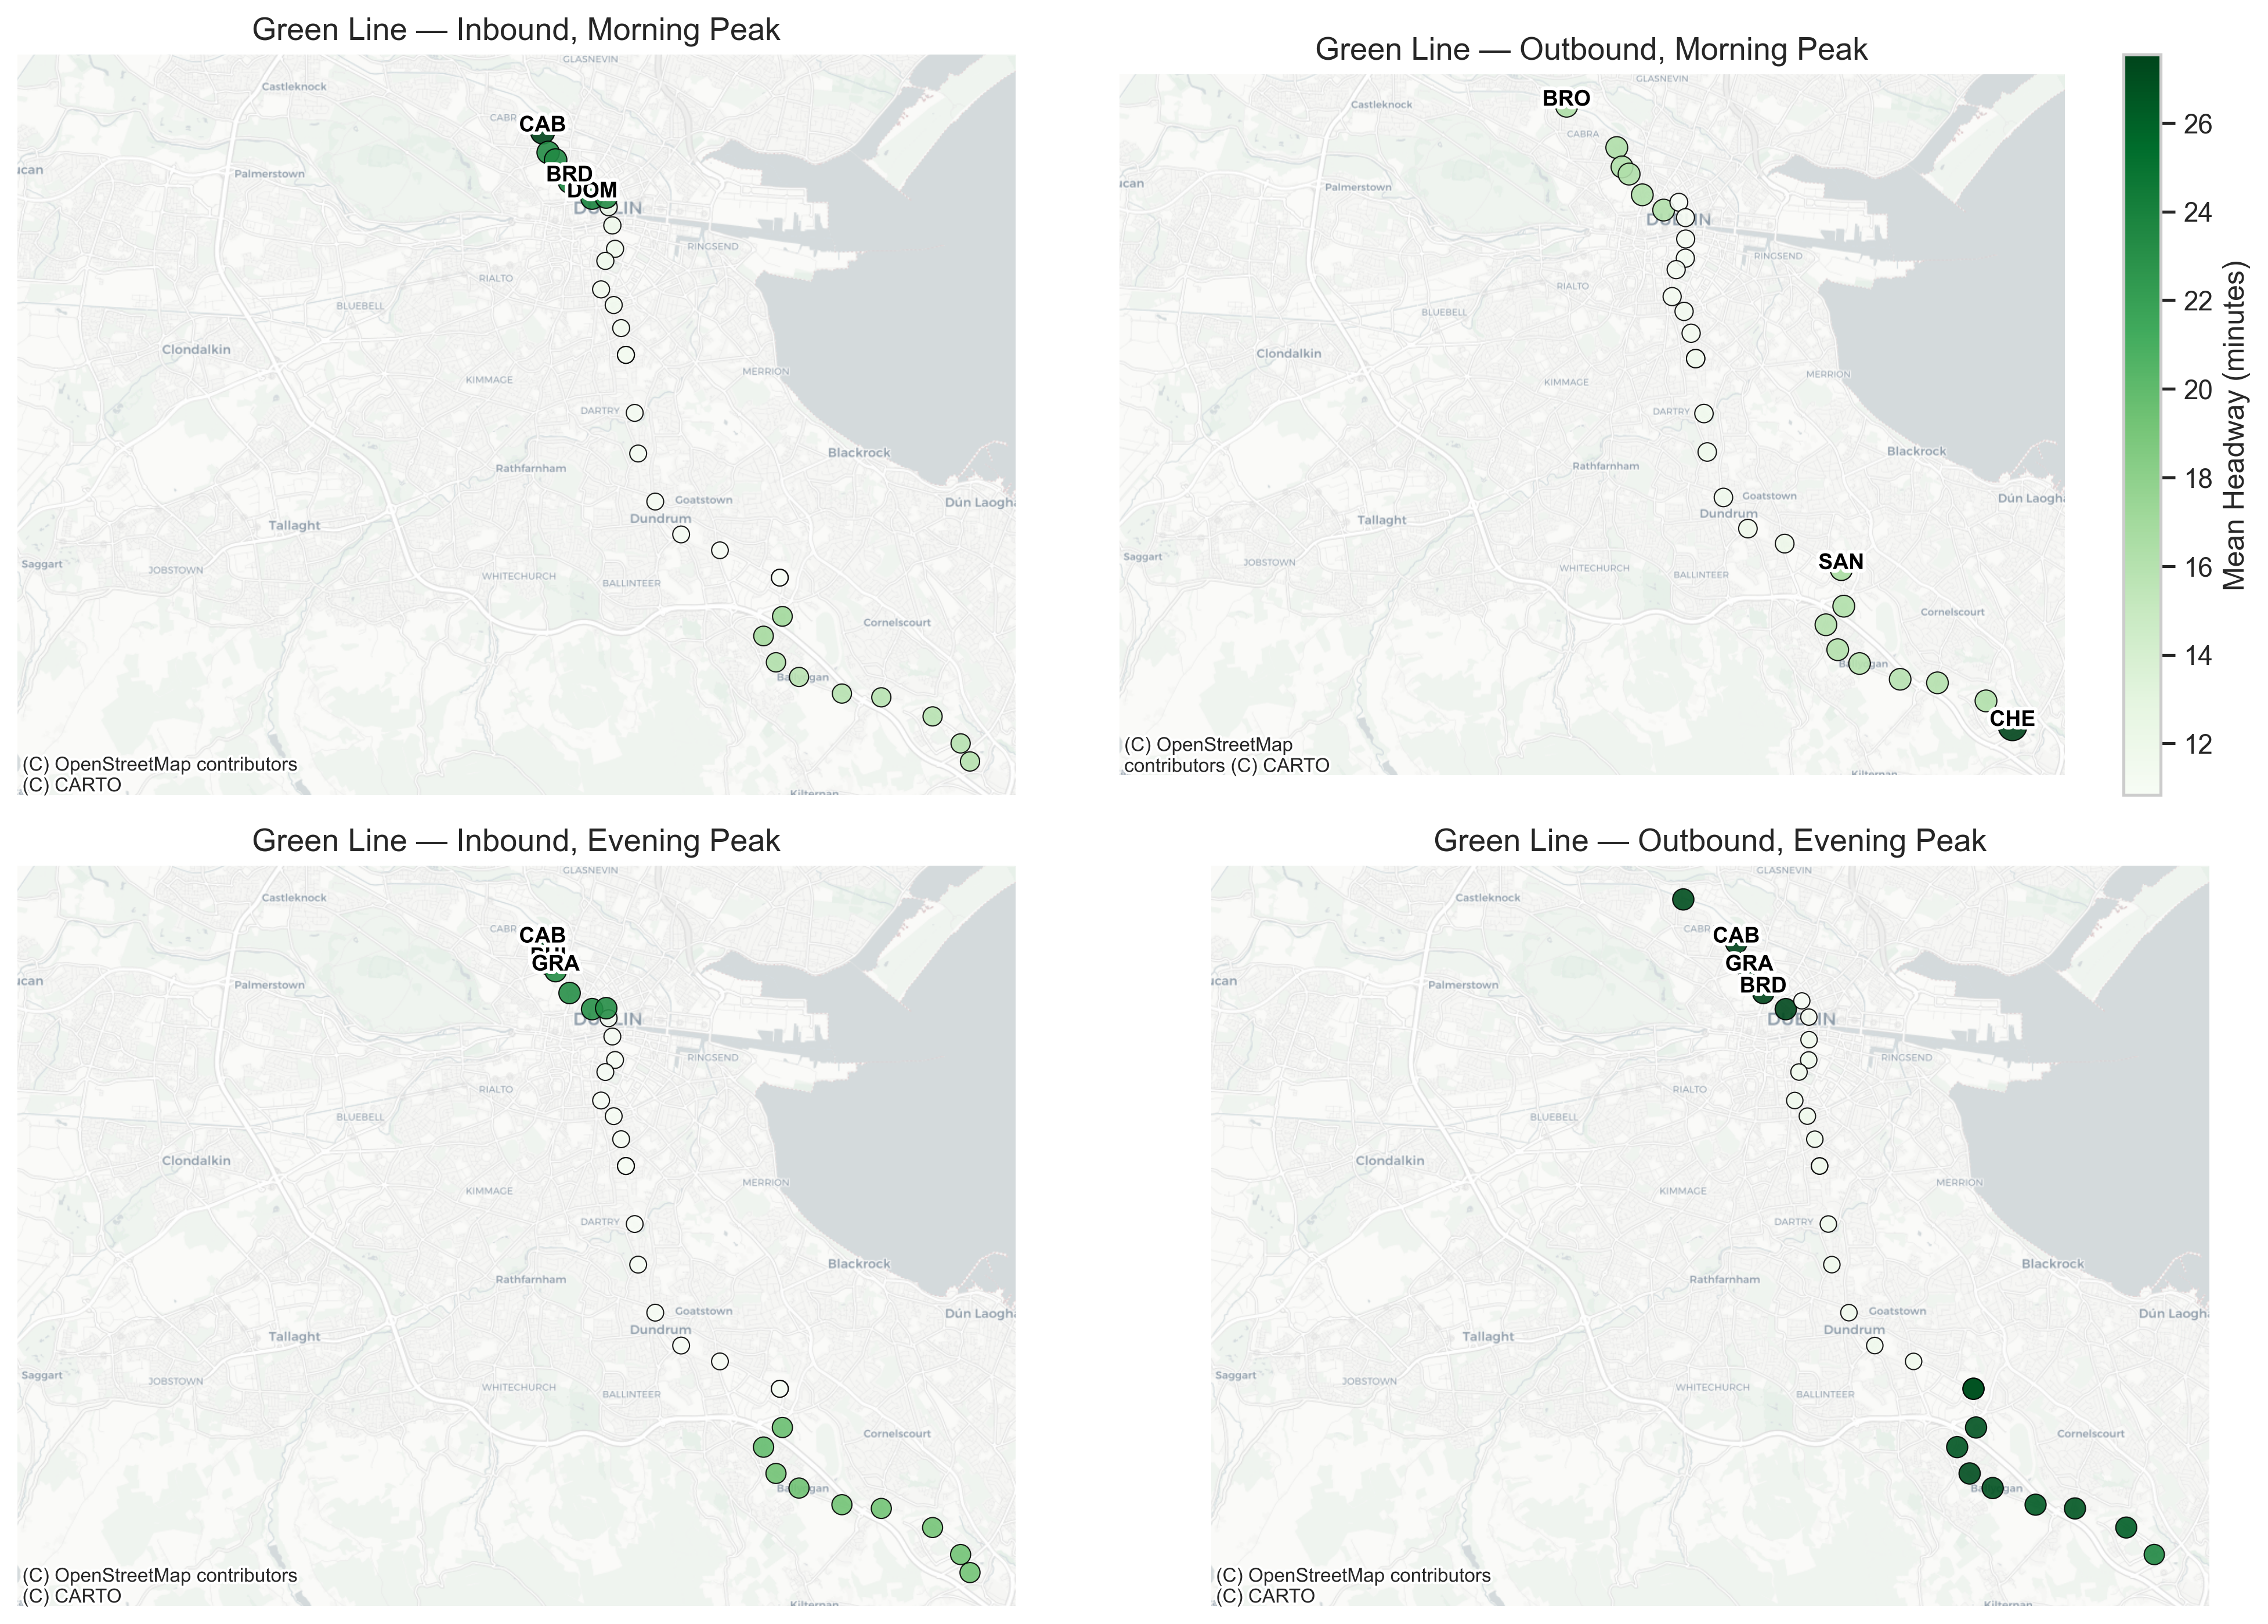
\includegraphics[width=0.49\textwidth]{figures/appendix_figures/headway_regularity/headways_combined_green_precovid.png}
  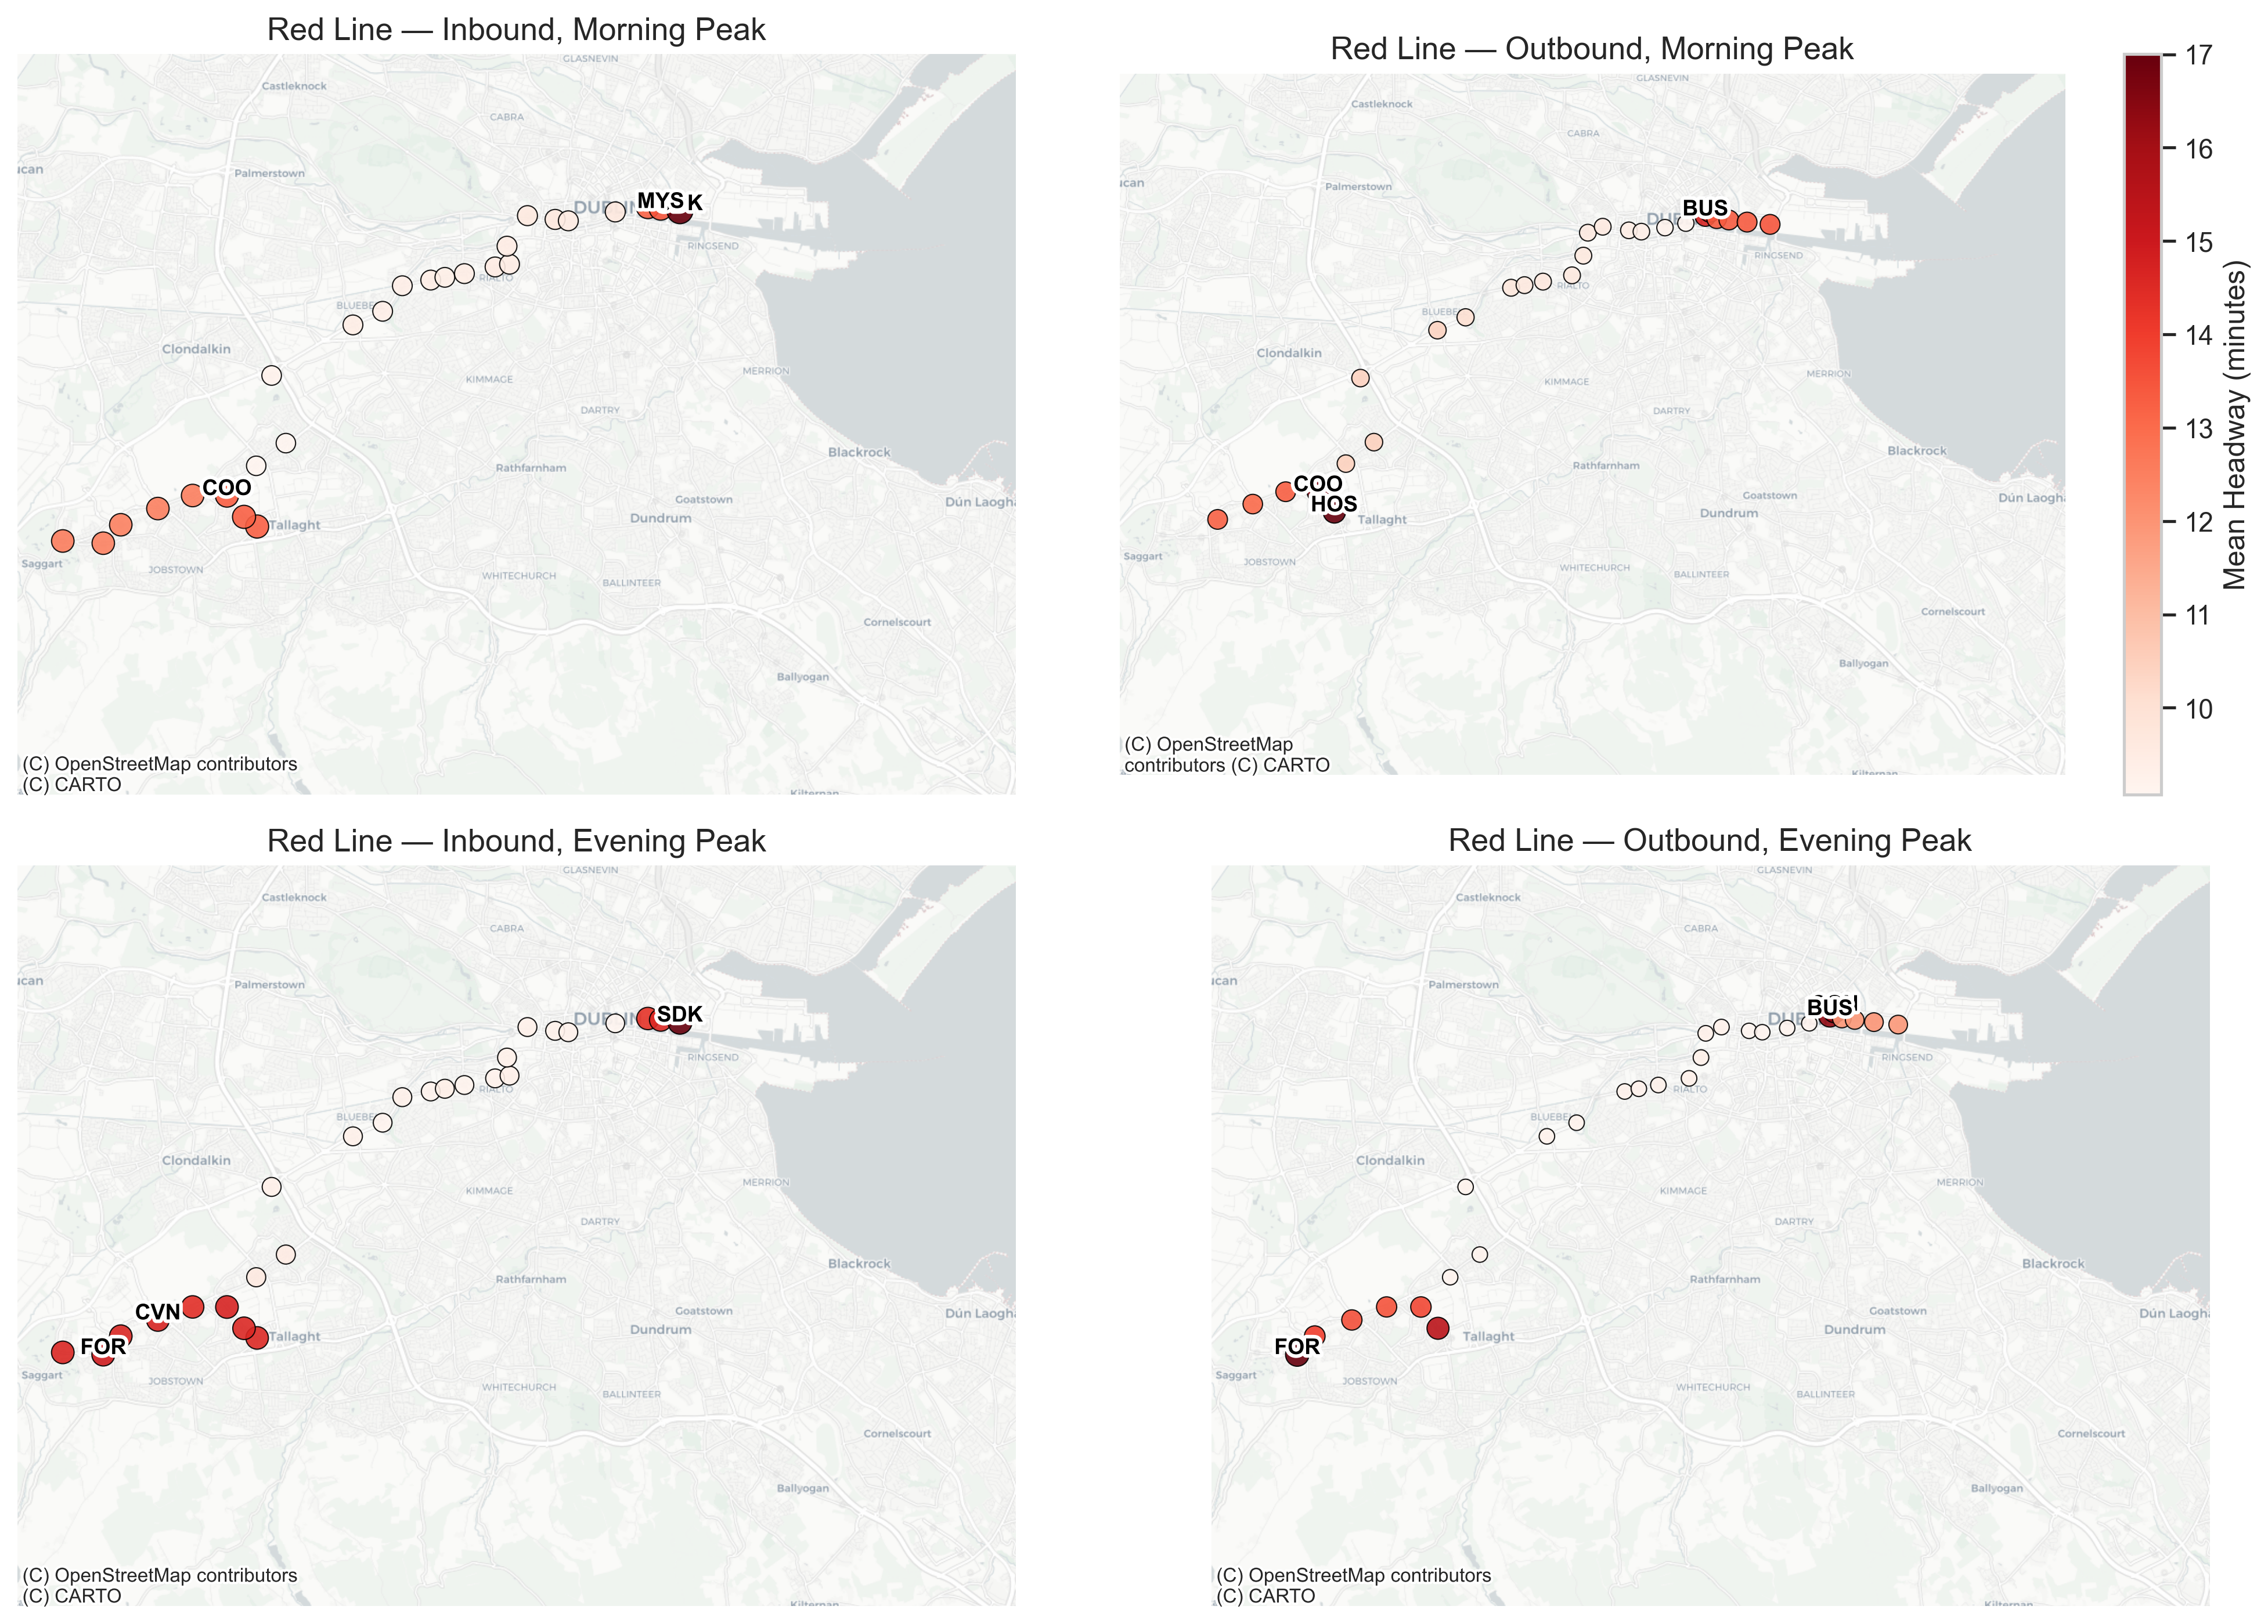
\includegraphics[width=0.49\textwidth]{figures/appendix_figures/headway_regularity/headways_combined_red_precovid.png}
  \caption{Pre-COVID}
\end{figure}

\begin{figure}[H]
  \centering
  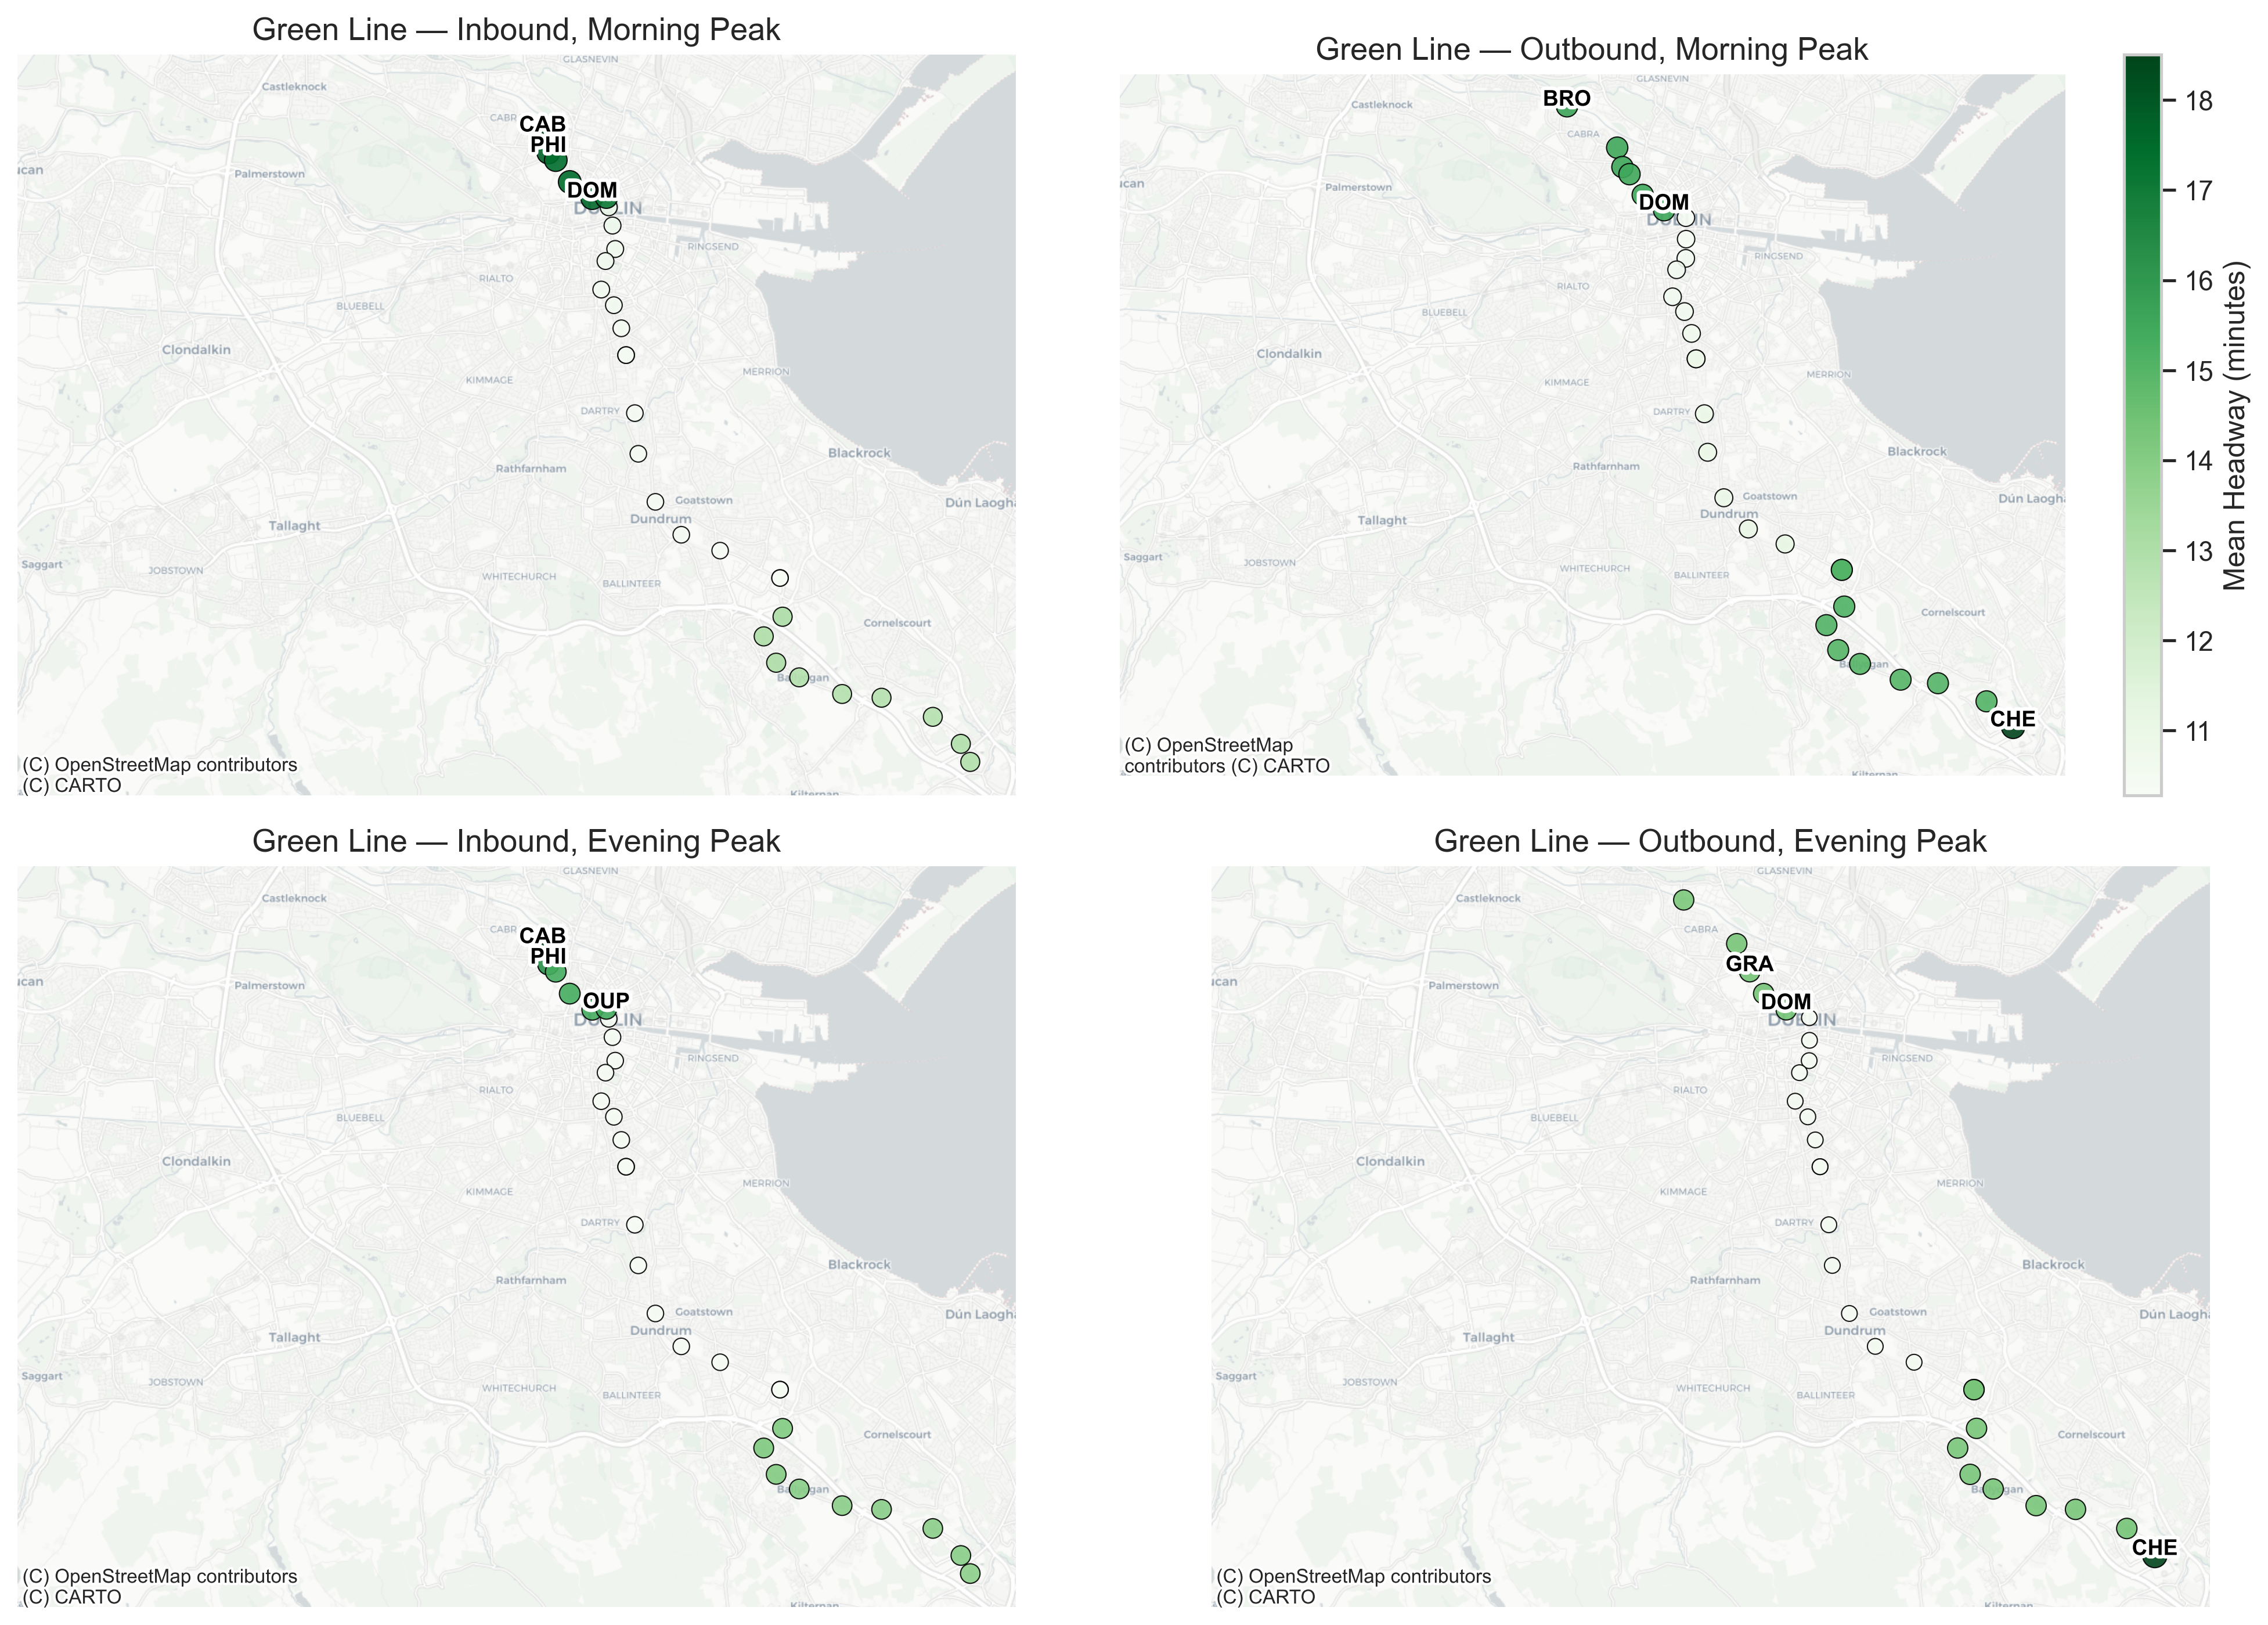
\includegraphics[width=0.49\textwidth]{figures/appendix_figures/headway_regularity/headways_combined_green_lockdown.png}
  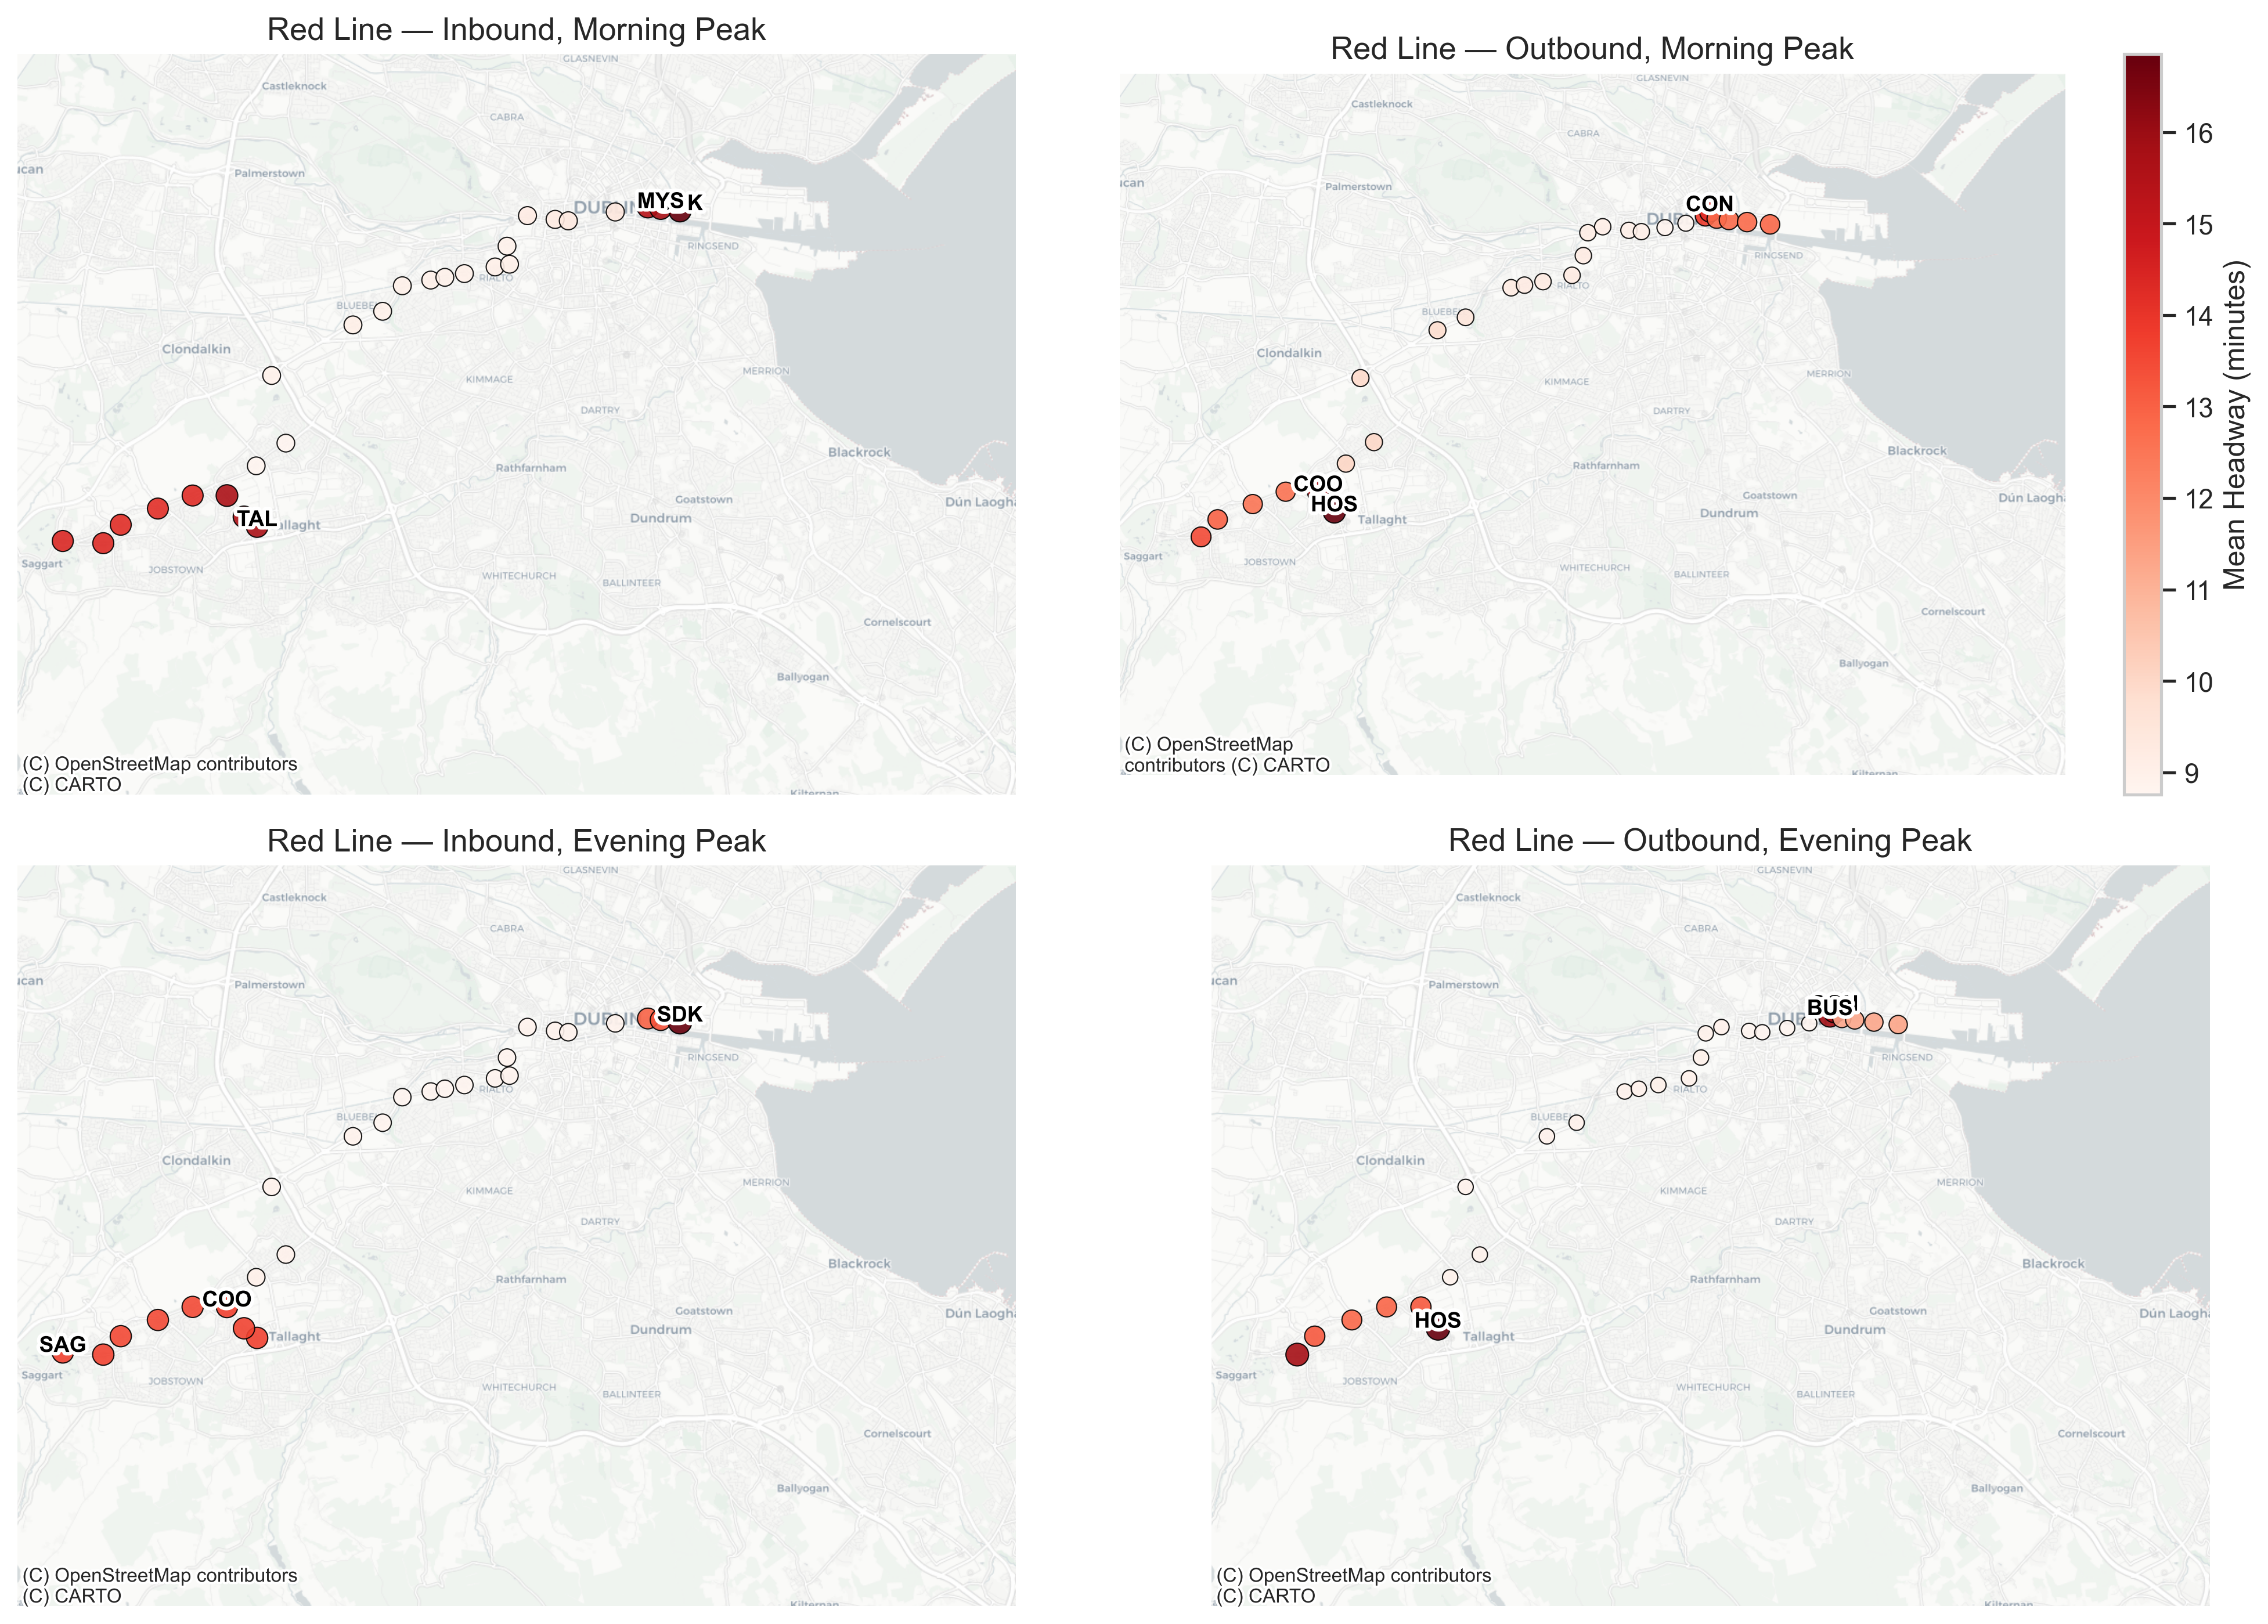
\includegraphics[width=0.49\textwidth]{figures/appendix_figures/headway_regularity/headways_combined_red_lockdown.png}
  \caption{Lockdown}
\end{figure}

\begin{figure}[H]
  \centering
  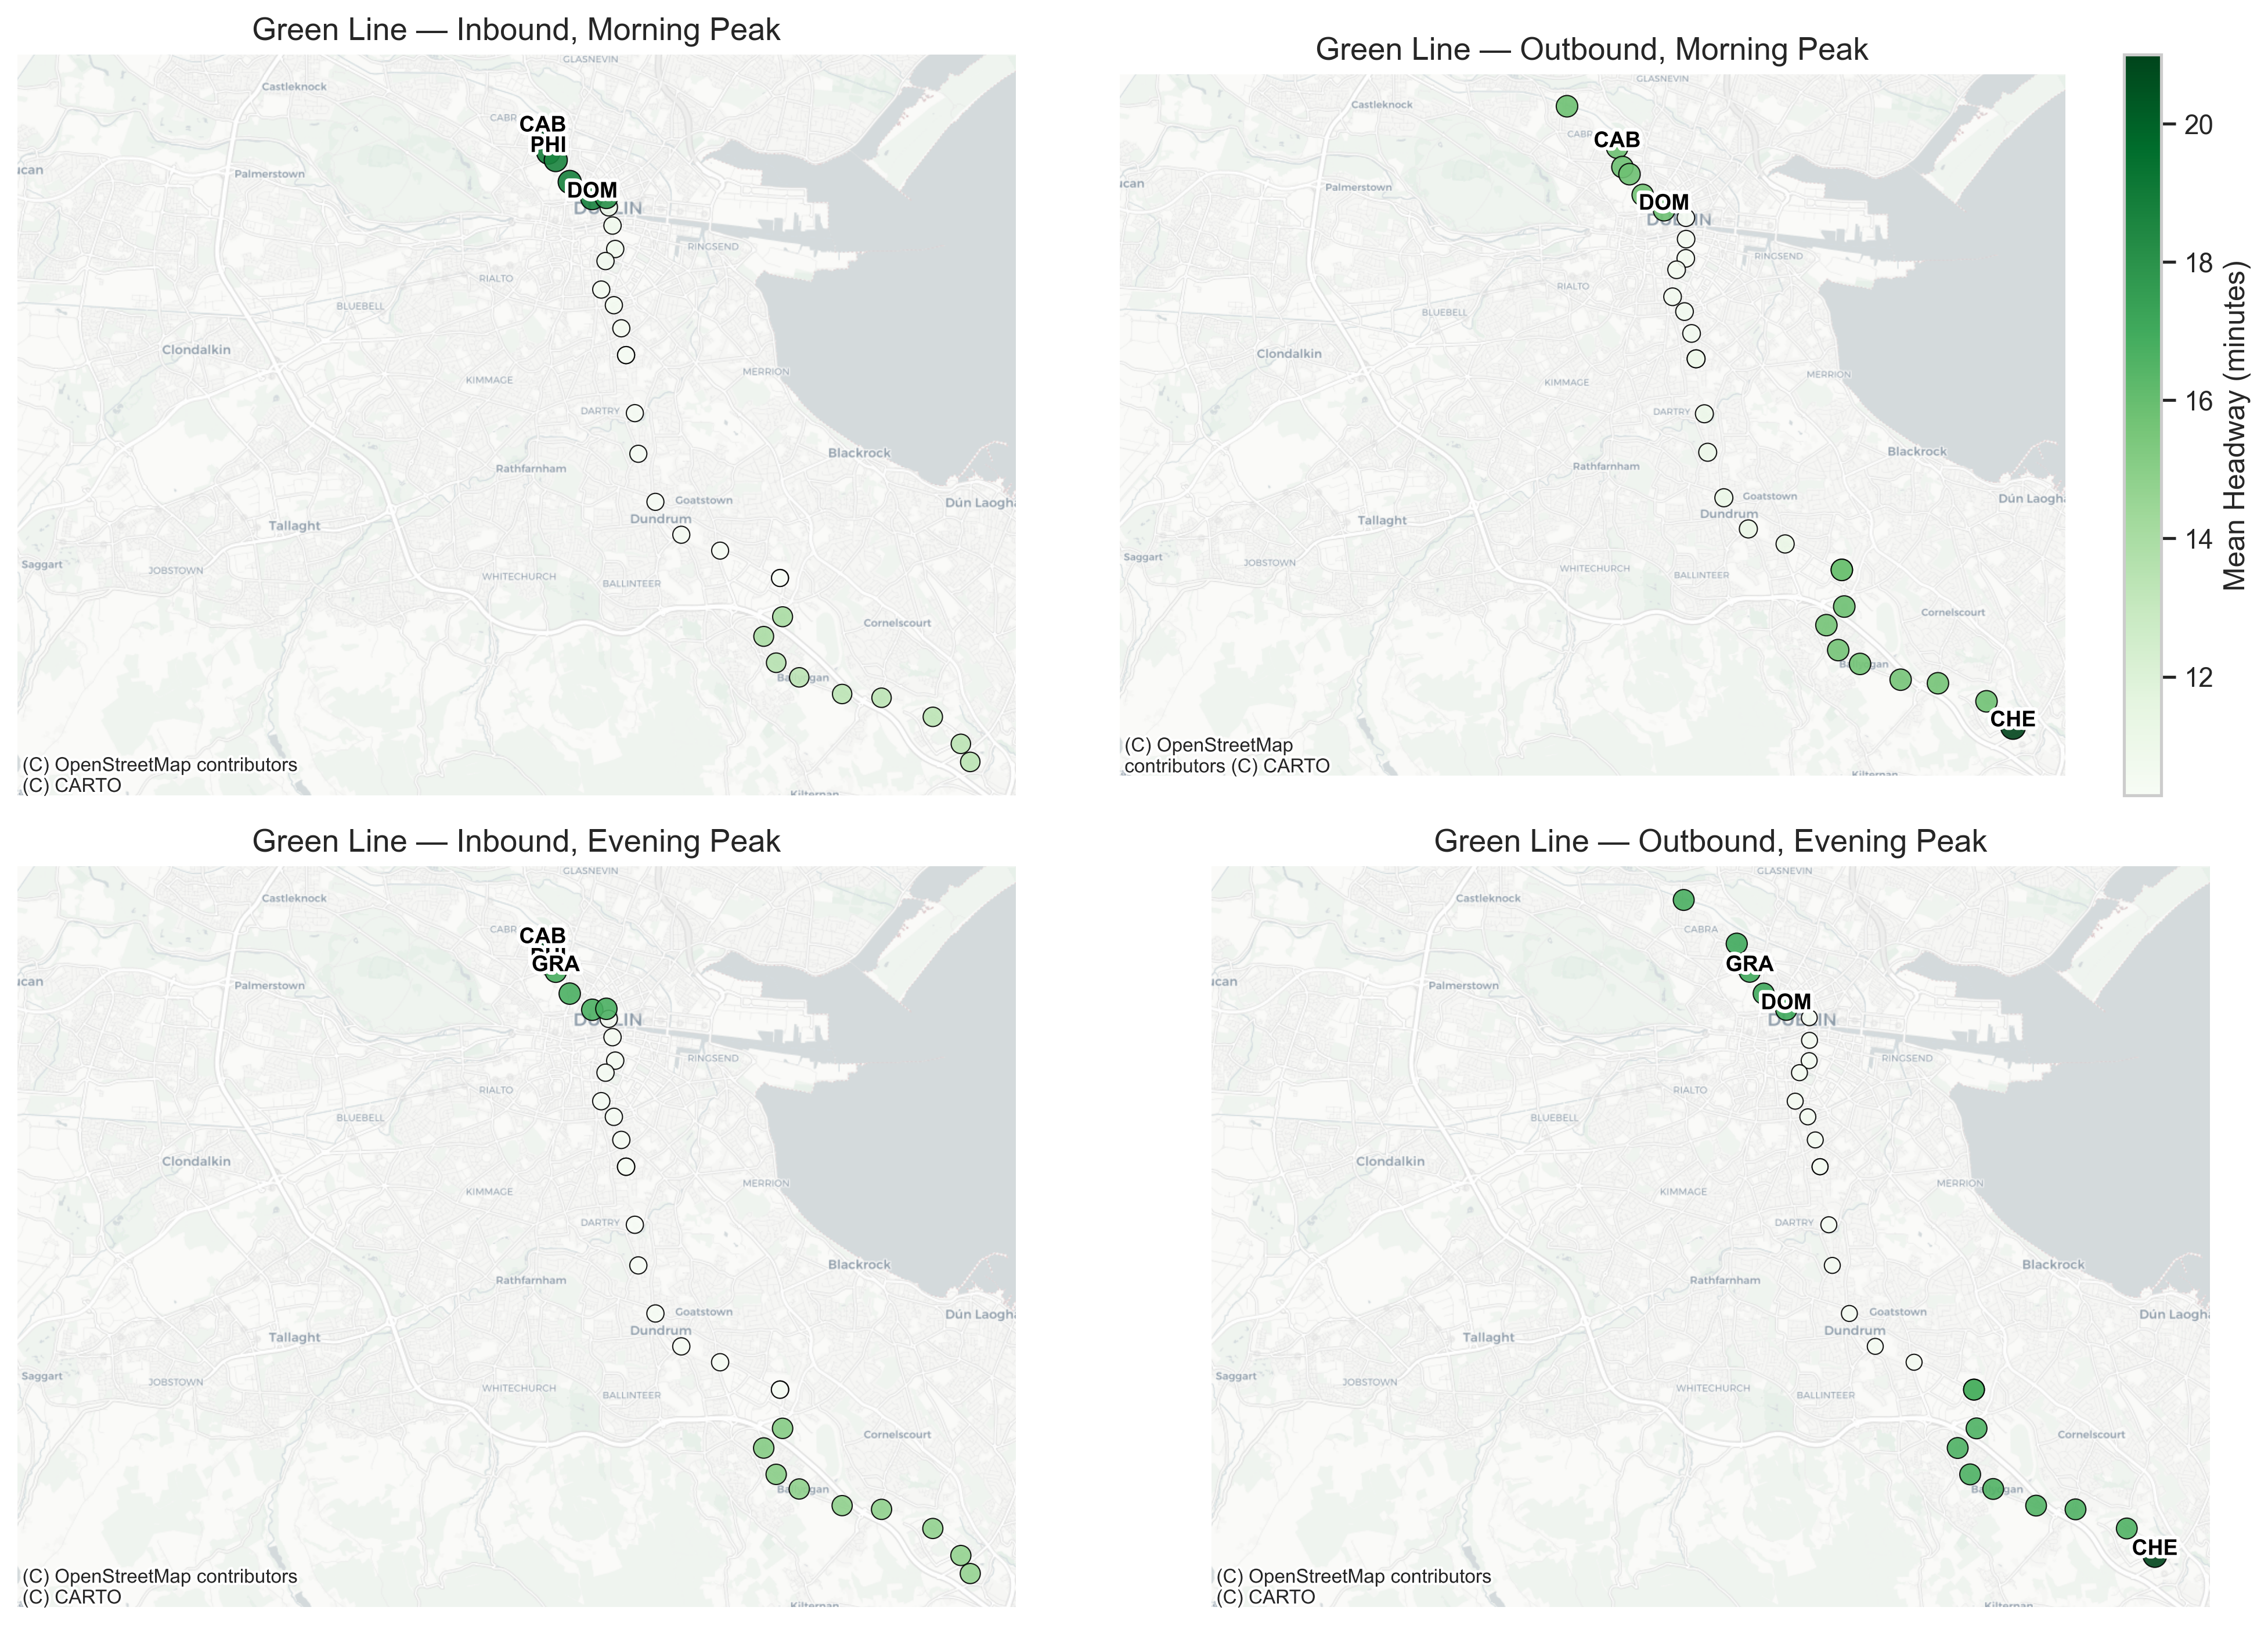
\includegraphics[width=0.49\textwidth]{figures/appendix_figures/headway_regularity/headways_combined_green_recovery.png}
  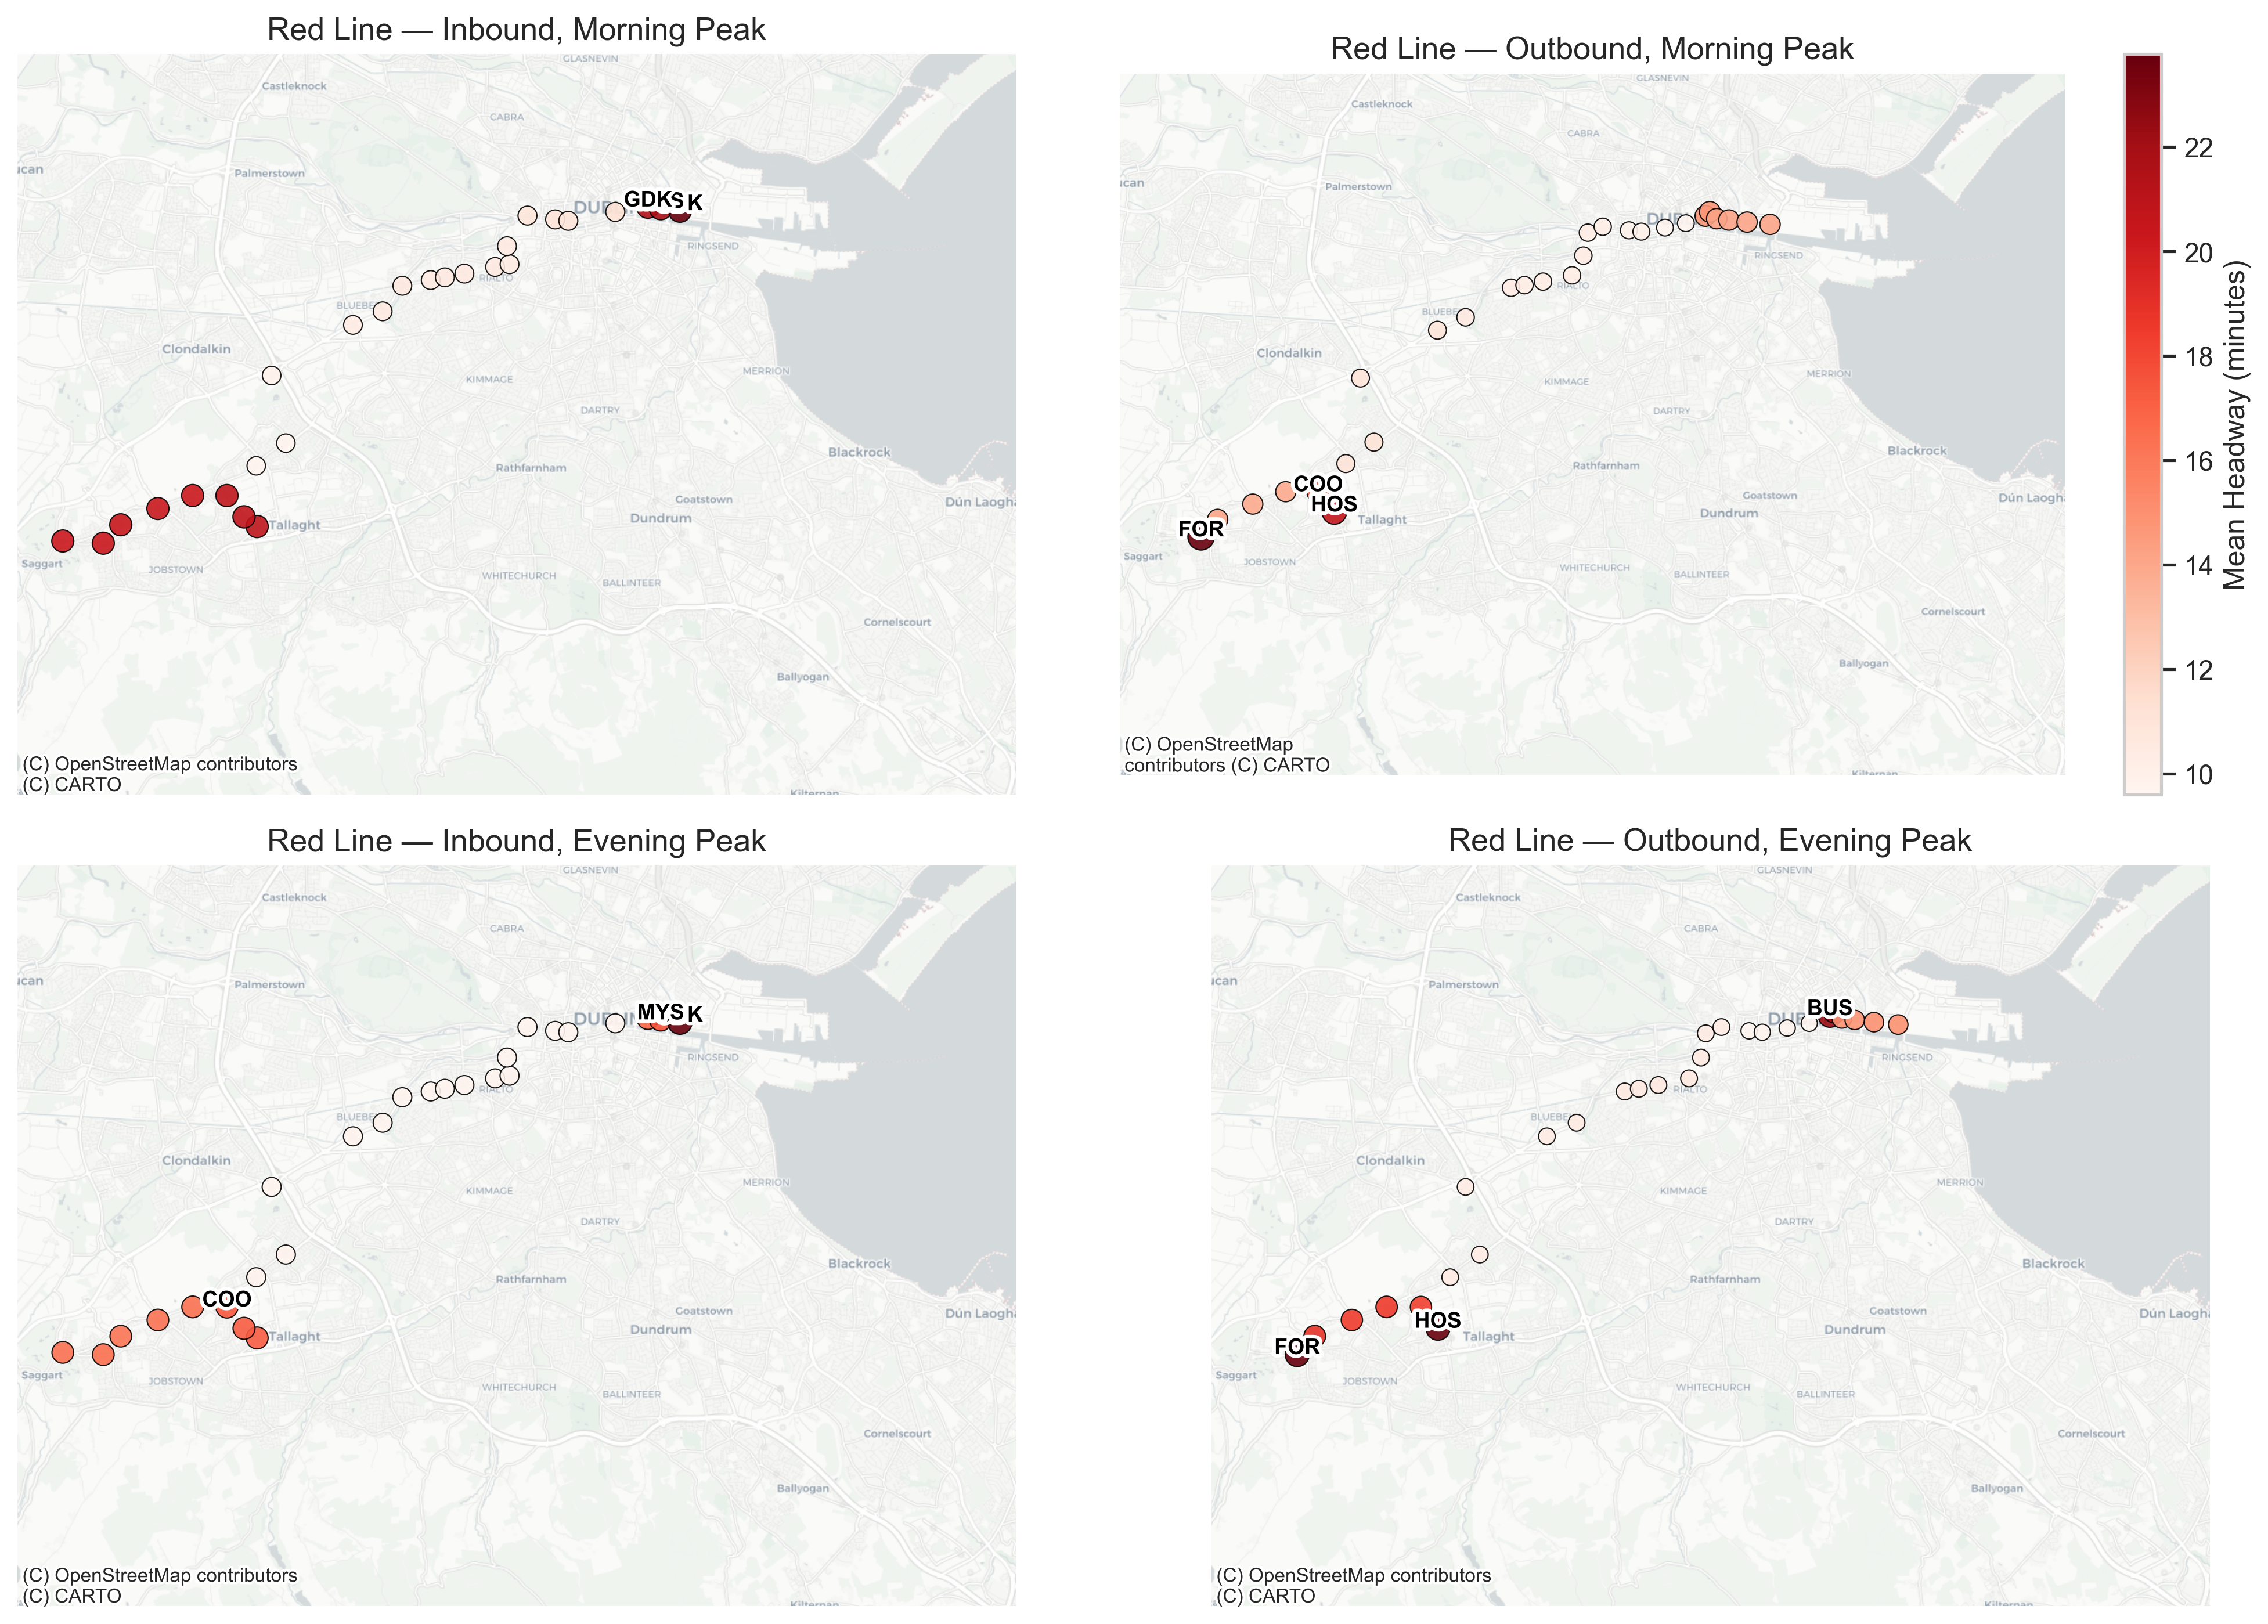
\includegraphics[width=0.49\textwidth]{figures/appendix_figures/headway_regularity/headways_combined_red_recovery.png}
  \caption{Recovery}
\end{figure}

\begin{figure}[H]
  \centering
  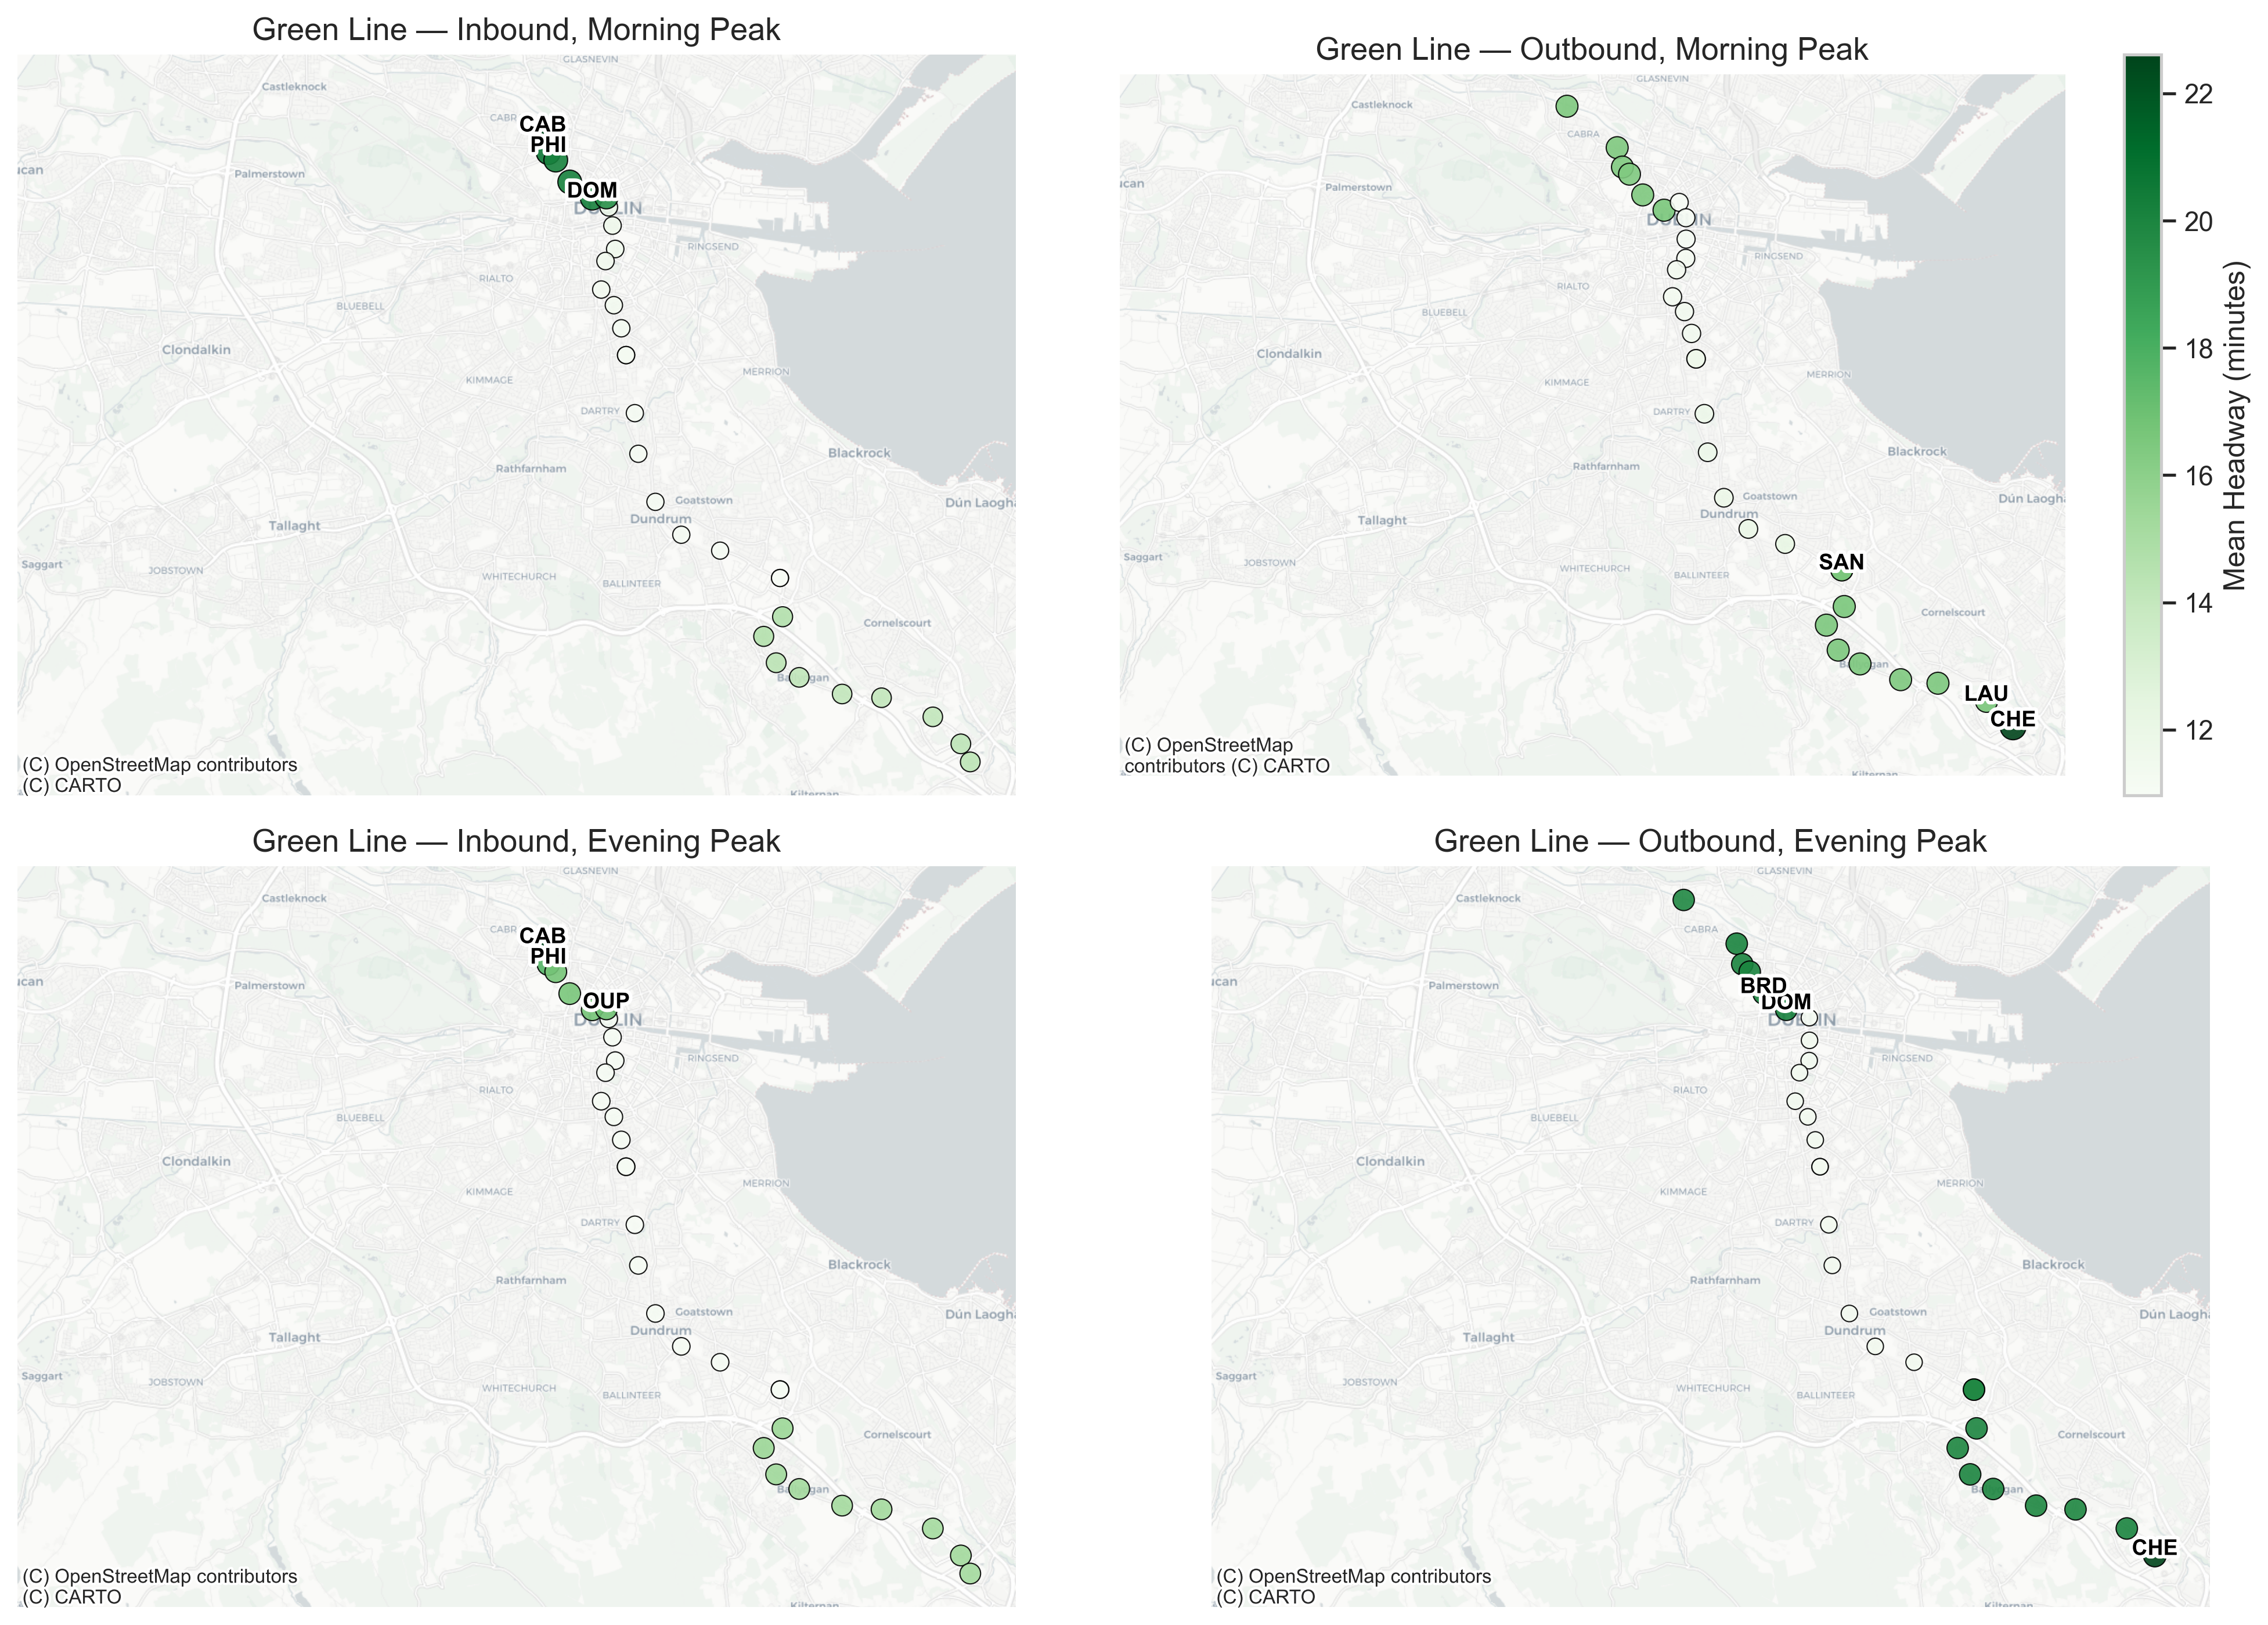
\includegraphics[width=0.49\textwidth]{figures/appendix_figures/headway_regularity/headways_combined_green_postcovid.png}
  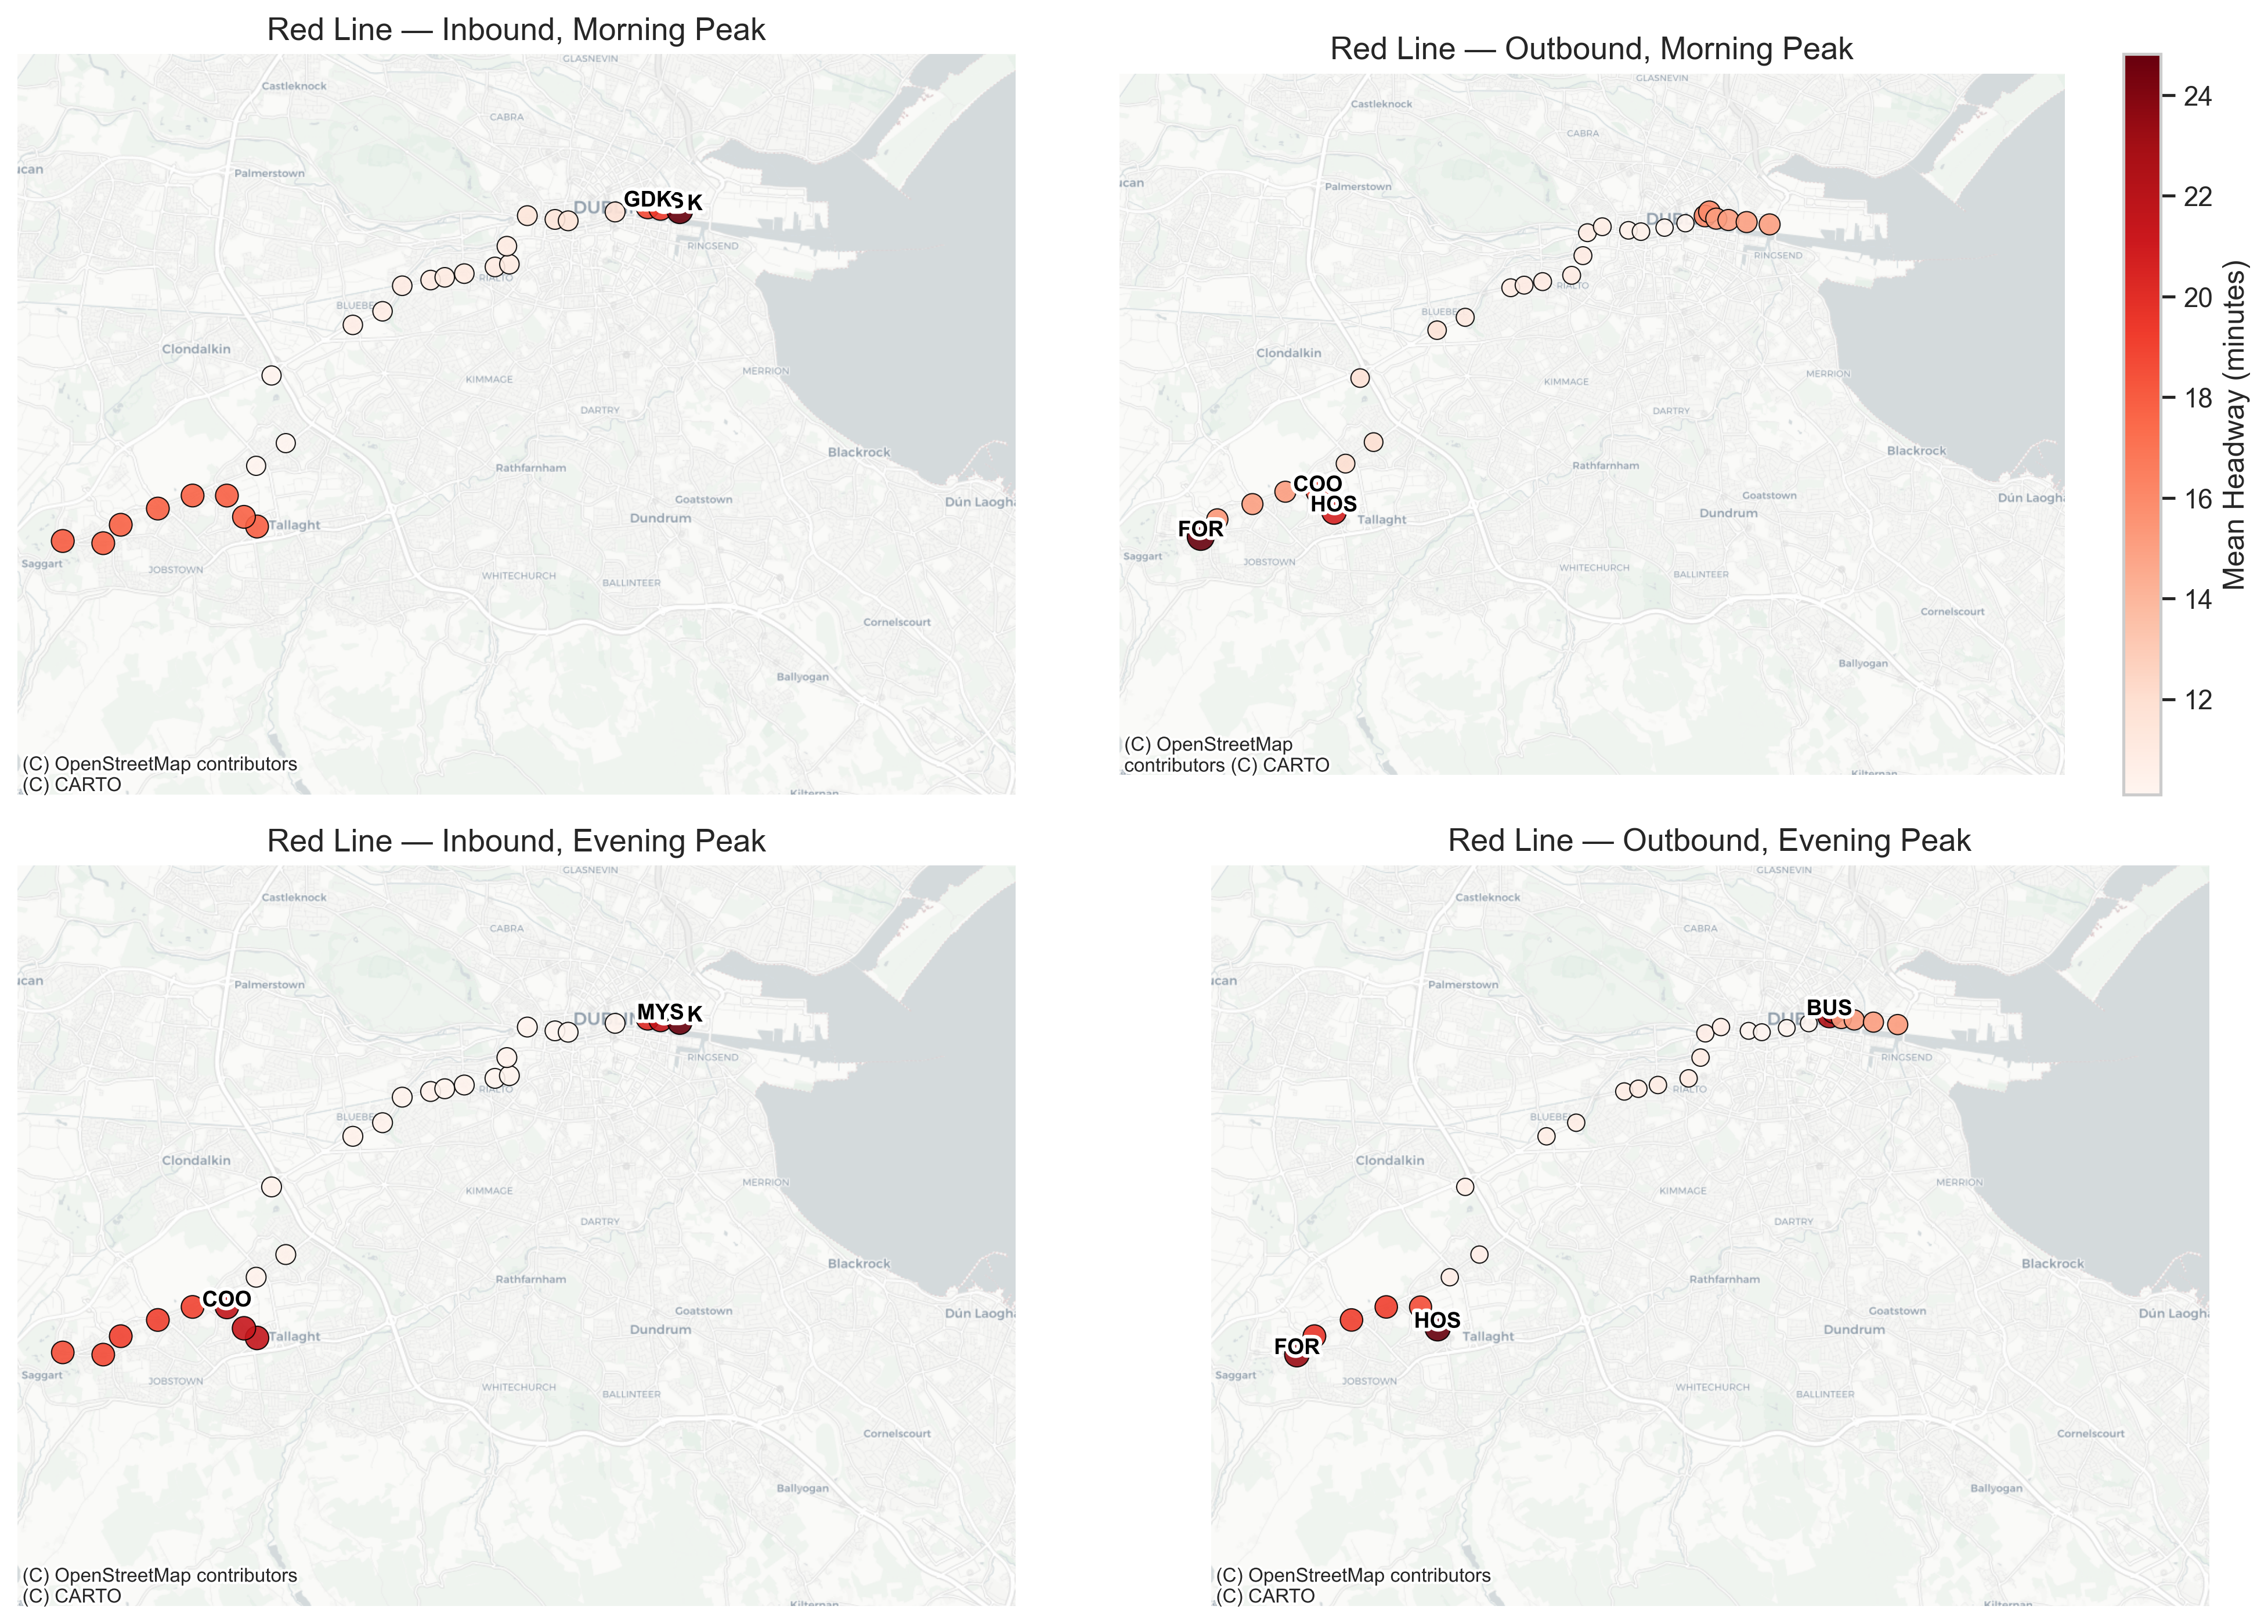
\includegraphics[width=0.49\textwidth]{figures/appendix_figures/headway_regularity/headways_combined_red_postcovid.png}
  \caption{Post-COVID}
\end{figure}

% --------------------------------------------------
\newpage
\subsection*{Travel Time Volatility}

\subsubsection*{Volatility Below the Threshold}
\begin{table}[H]
  \centering
  \caption{Percentage of stop-pairs with travel time volatility (TTV) below 1 minute}
  \label{tab:ttv_summary}
  \begin{tabular}{lcc}
    \textbf{Phase} & \textbf{\% Below 1 Min} & \textbf{Max Volatility (min)} \\
    Pre-COVID & 77.66 & 4.28 \\
    Lockdown  & 74.56 & 4.94 \\
    Recovery  & 73.84 & 4.27 \\
    Post-COVID & 72.63 & 4.24 \\
  \end{tabular}
\end{table}

\subsubsection*{Travel Time Volatility Figures}

\begin{figure}[H]
  \centering
  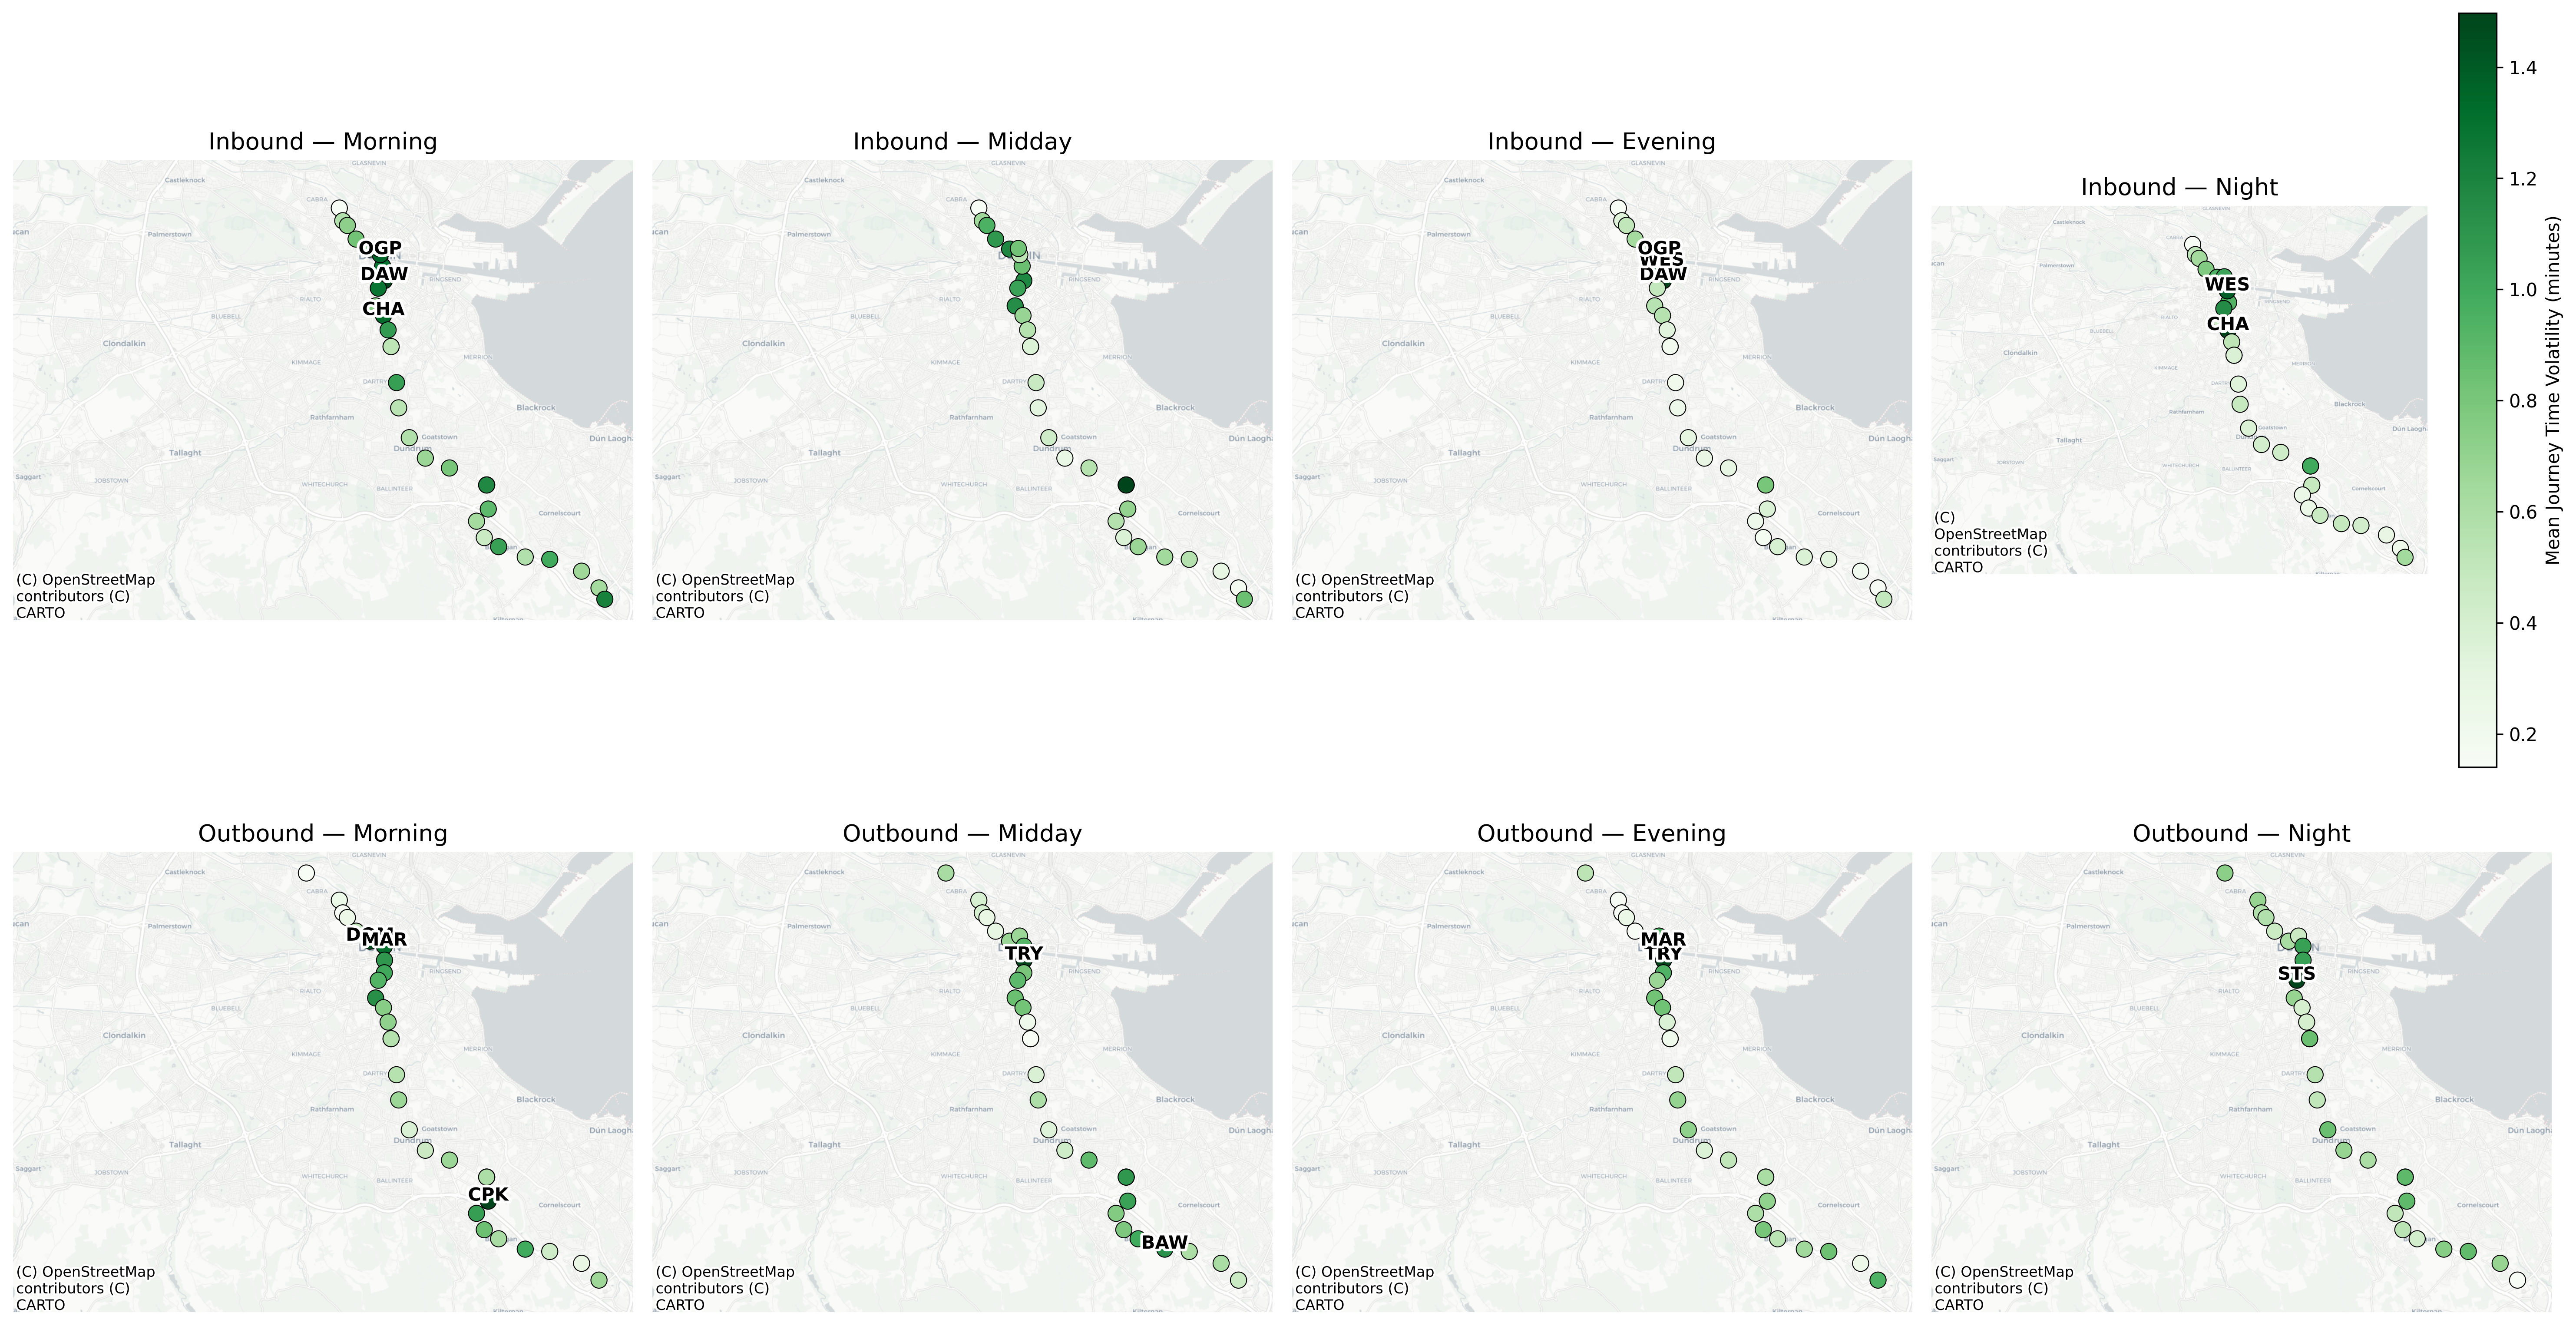
\includegraphics[width=0.85\textwidth]{figures/appendix_figures/travel_time_volatility/volatility_allperiods_green_combined_precovid.png}
  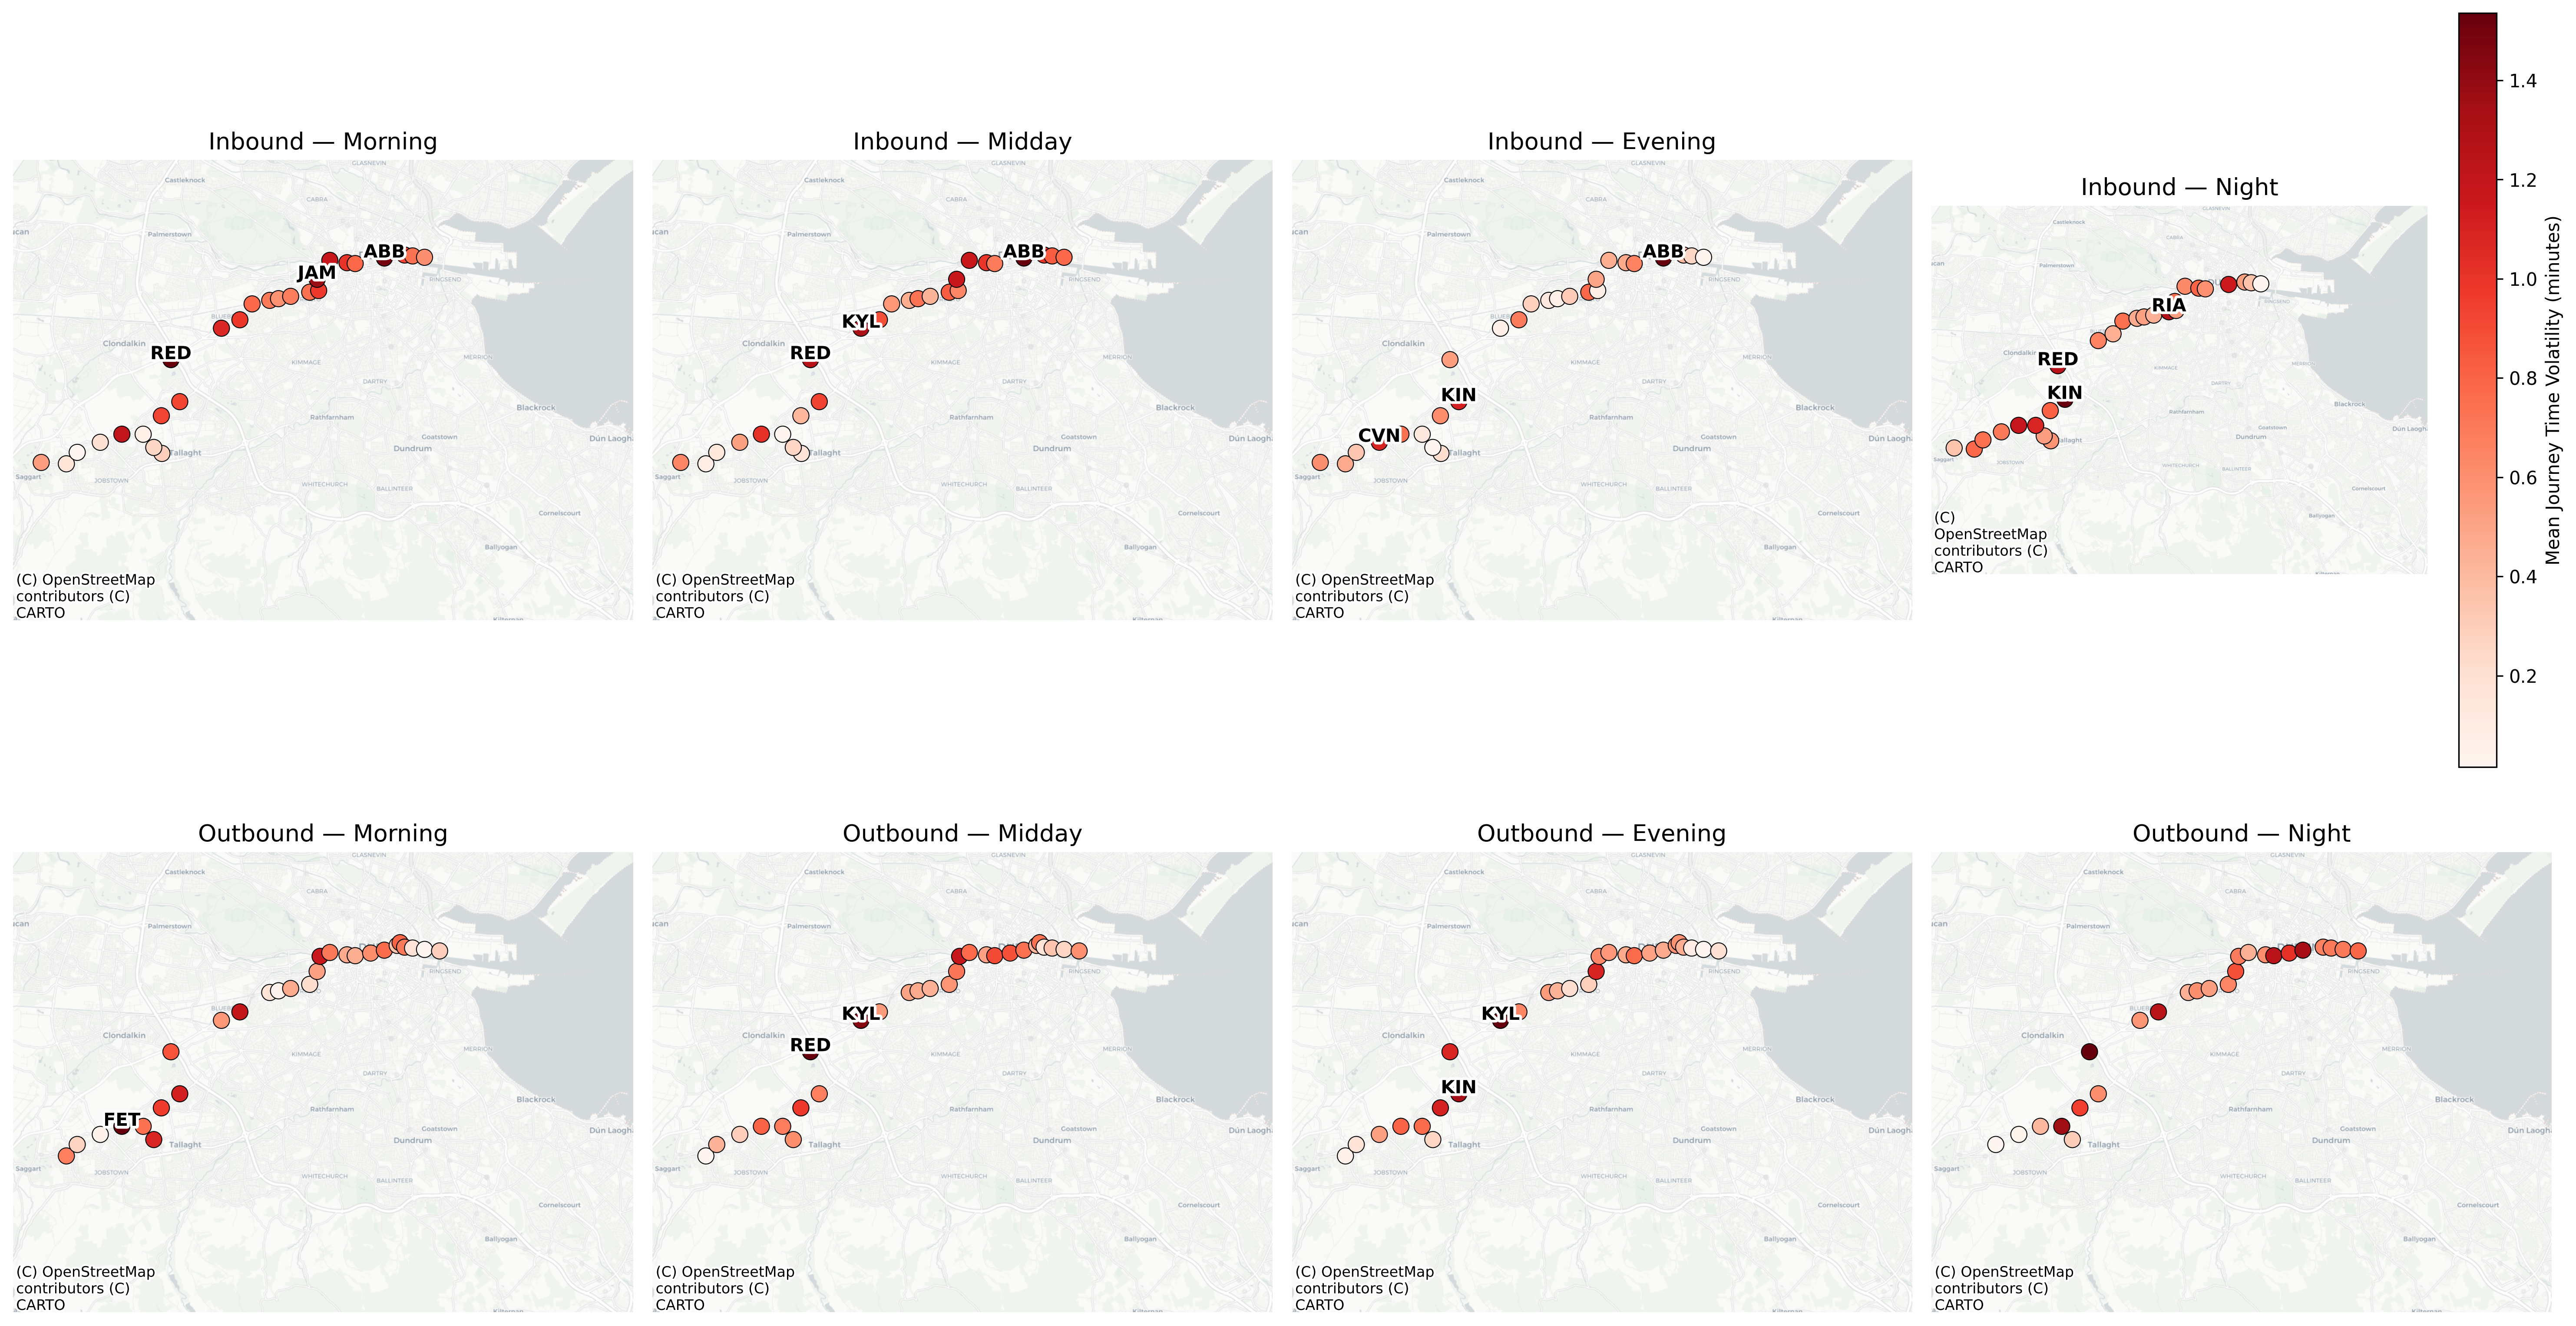
\includegraphics[width=0.85\textwidth]{figures/appendix_figures/travel_time_volatility/volatility_allperiods_red_combined_precovid.png}
  \caption{Pre-COVID}
\end{figure}

\vspace{5cm}
\begin{figure}[H]
  \centering
  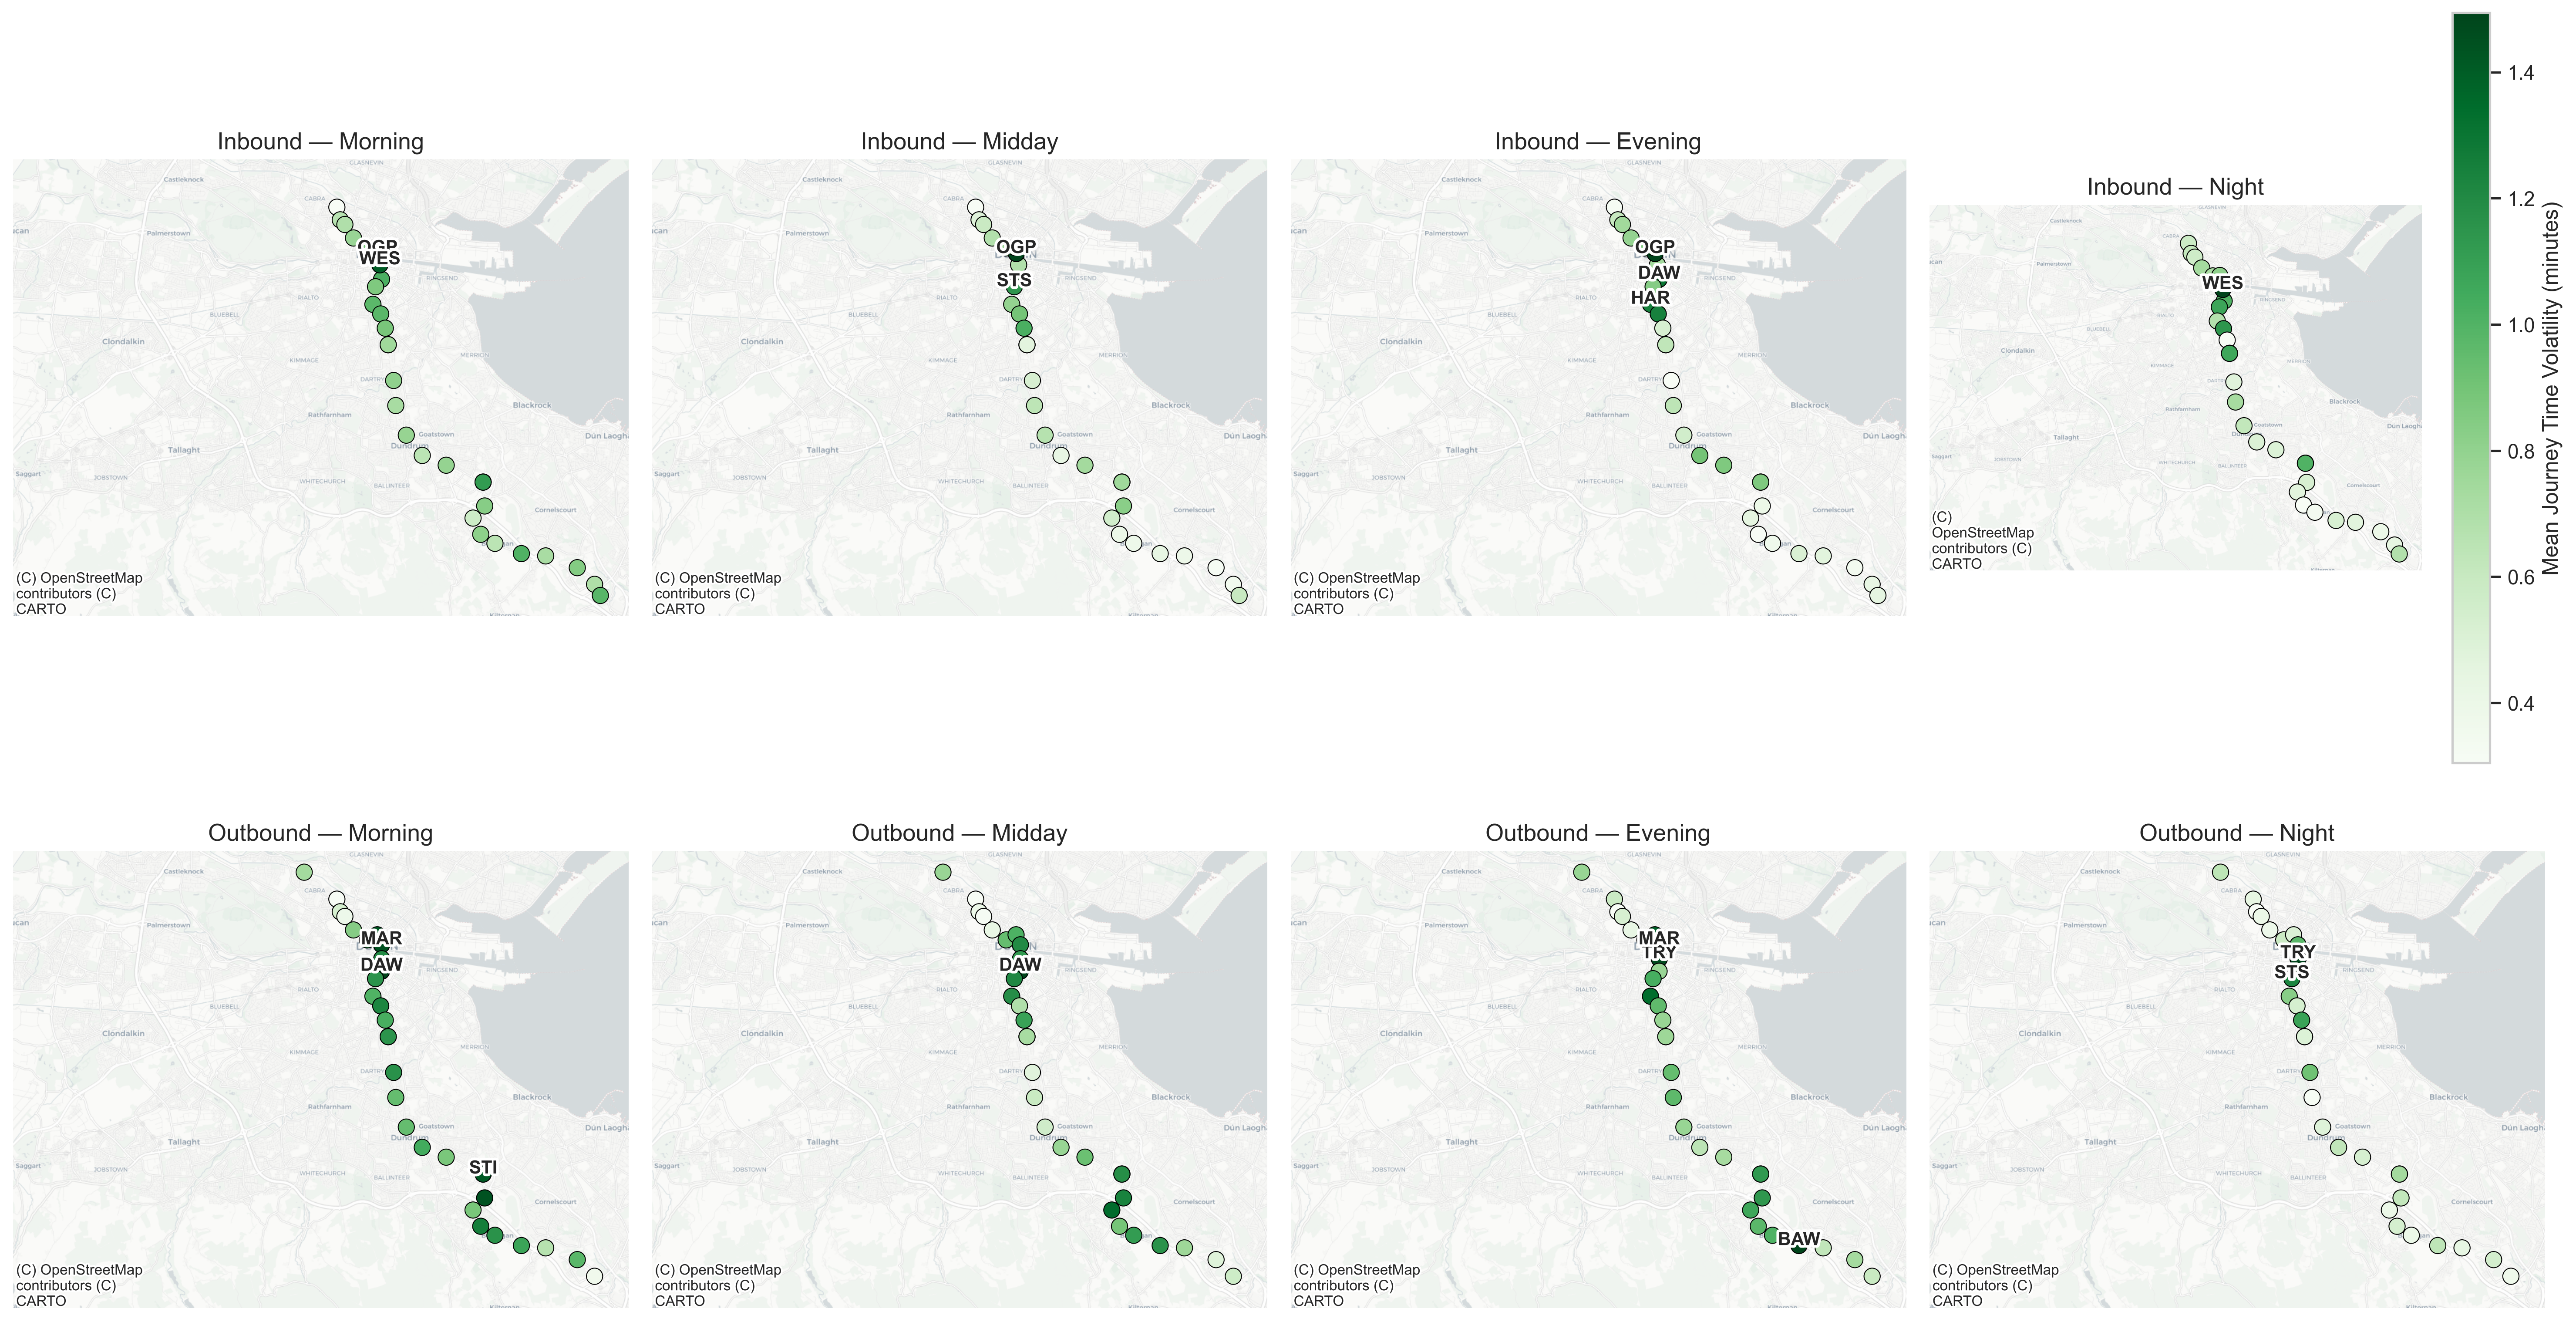
\includegraphics[width=0.85\textwidth]{figures/appendix_figures/travel_time_volatility/volatility_allperiods_green_combined_lockdown.png}
  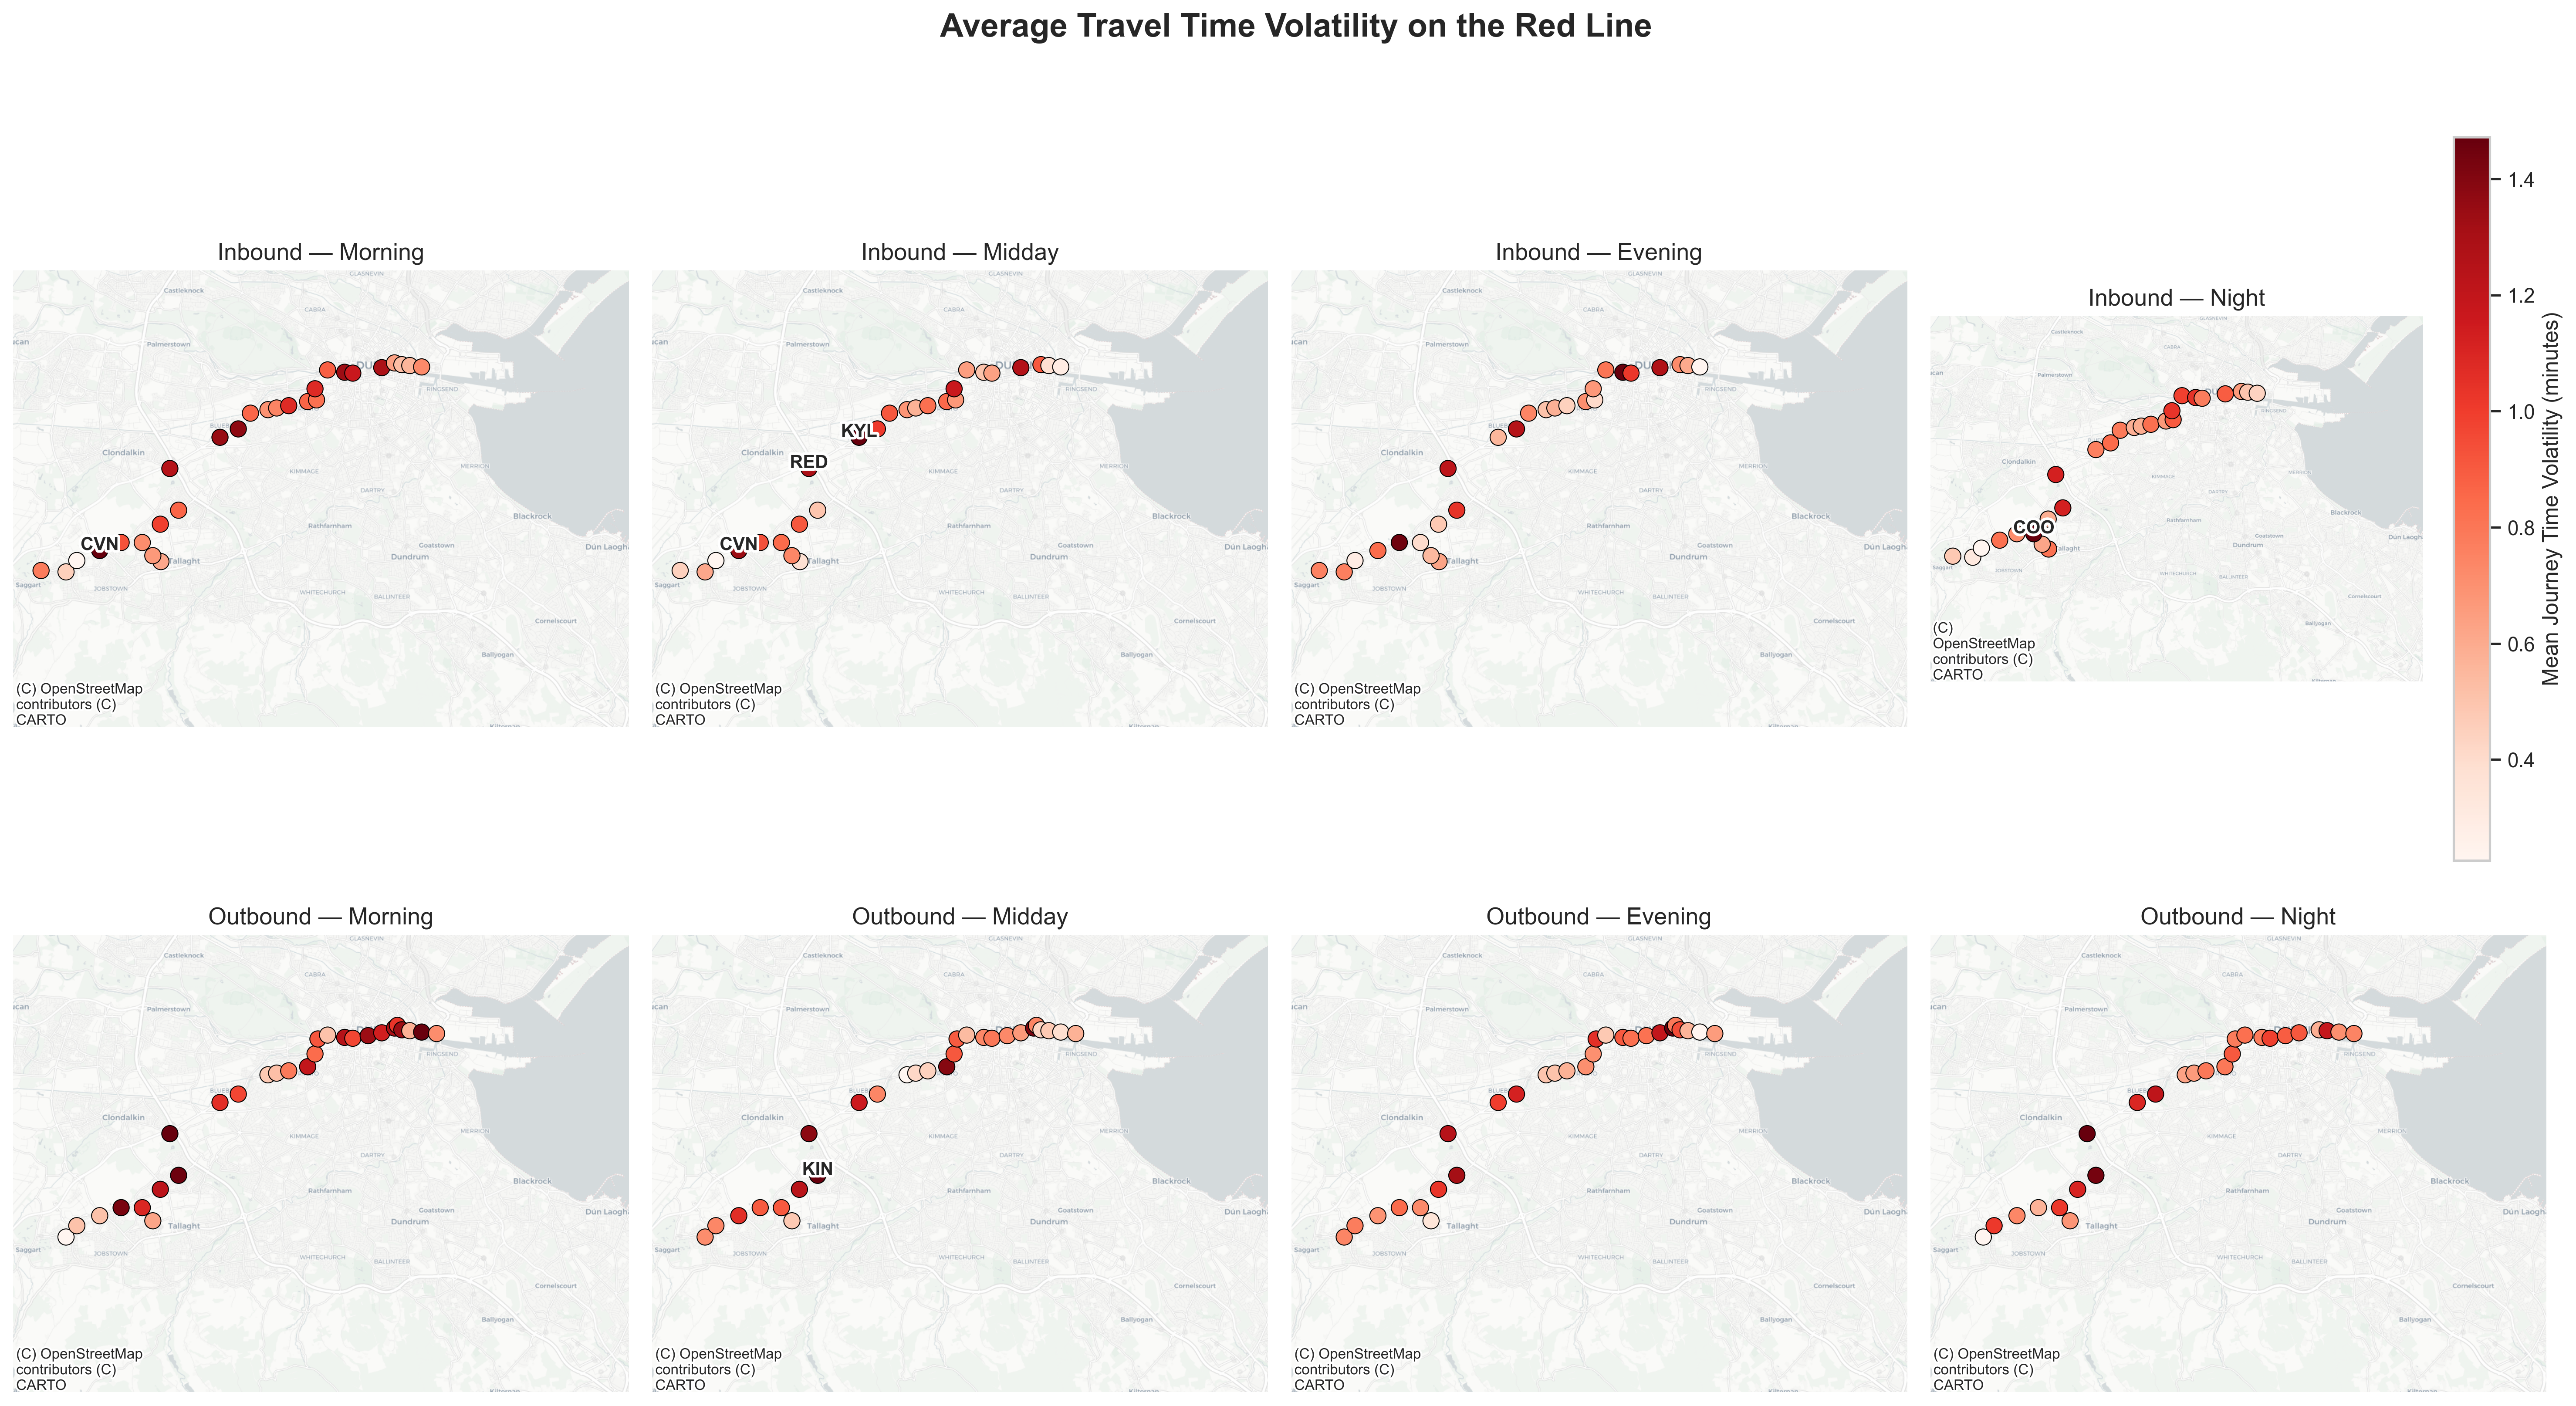
\includegraphics[width=0.85\textwidth]{figures/appendix_figures/travel_time_volatility/volatility_allperiods_red_combined_lockdown.png}
  \caption{Lockdown}
\end{figure}

\vspace{5cm}

\begin{figure}[H]
  \centering
  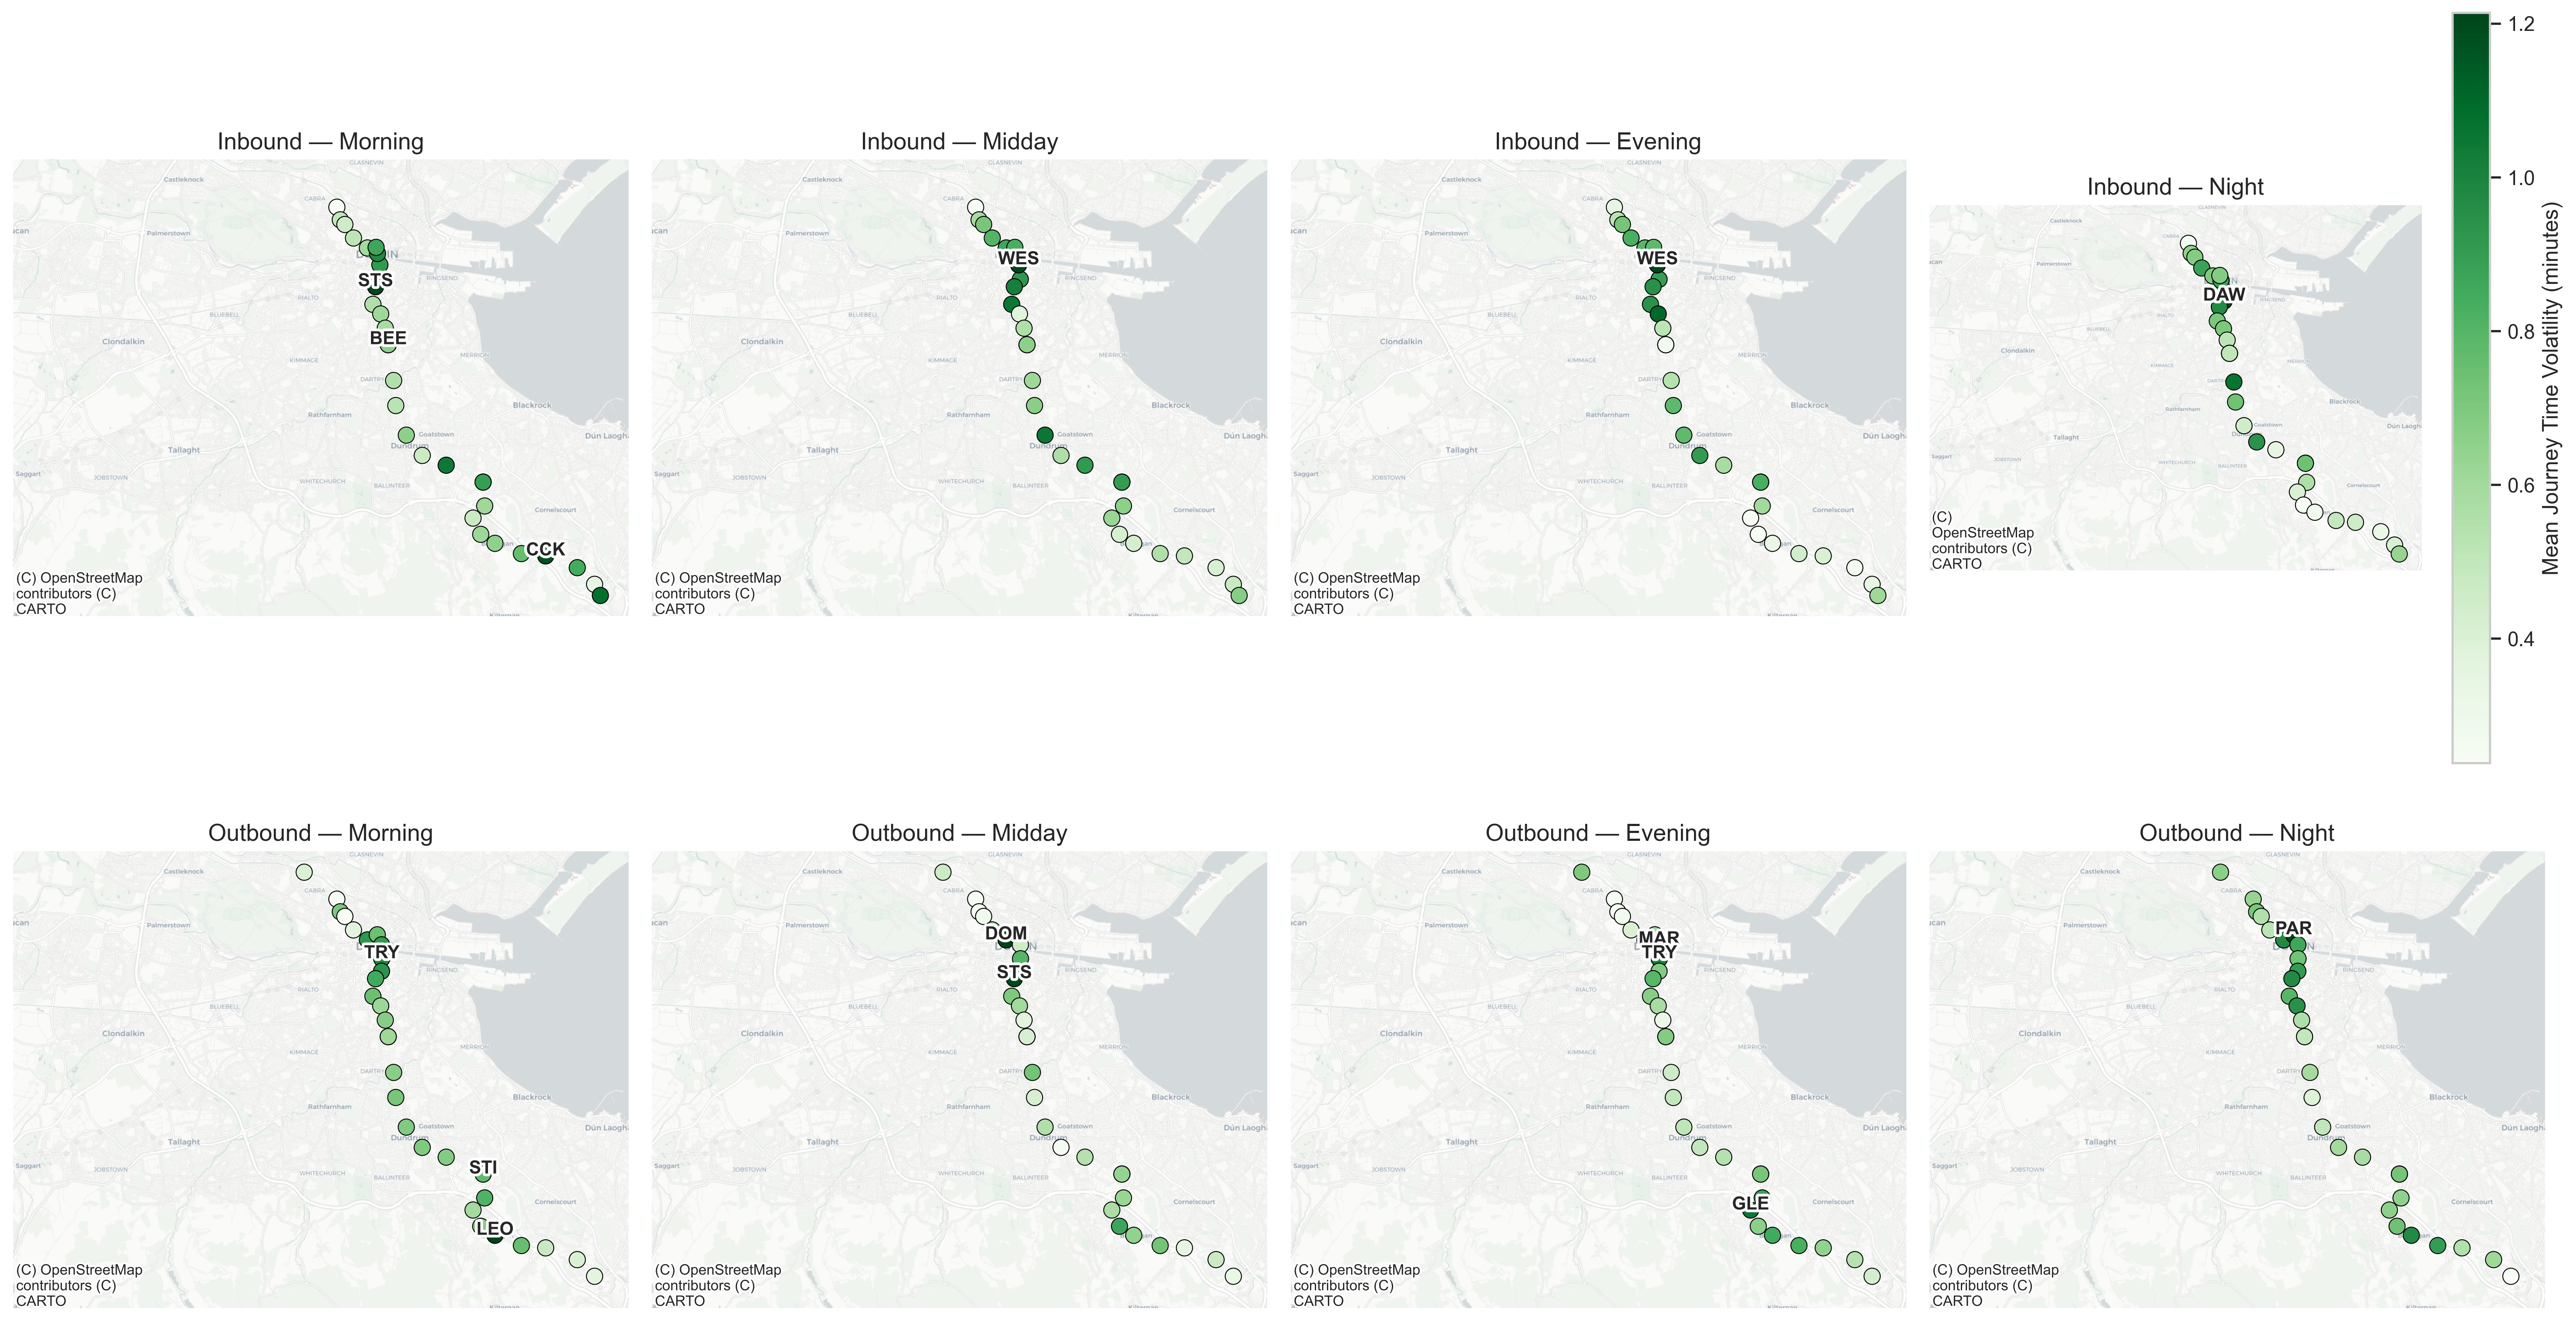
\includegraphics[width=0.85\textwidth]{figures/appendix_figures/travel_time_volatility/volatility_allperiods_green_combined_recovery.png}
  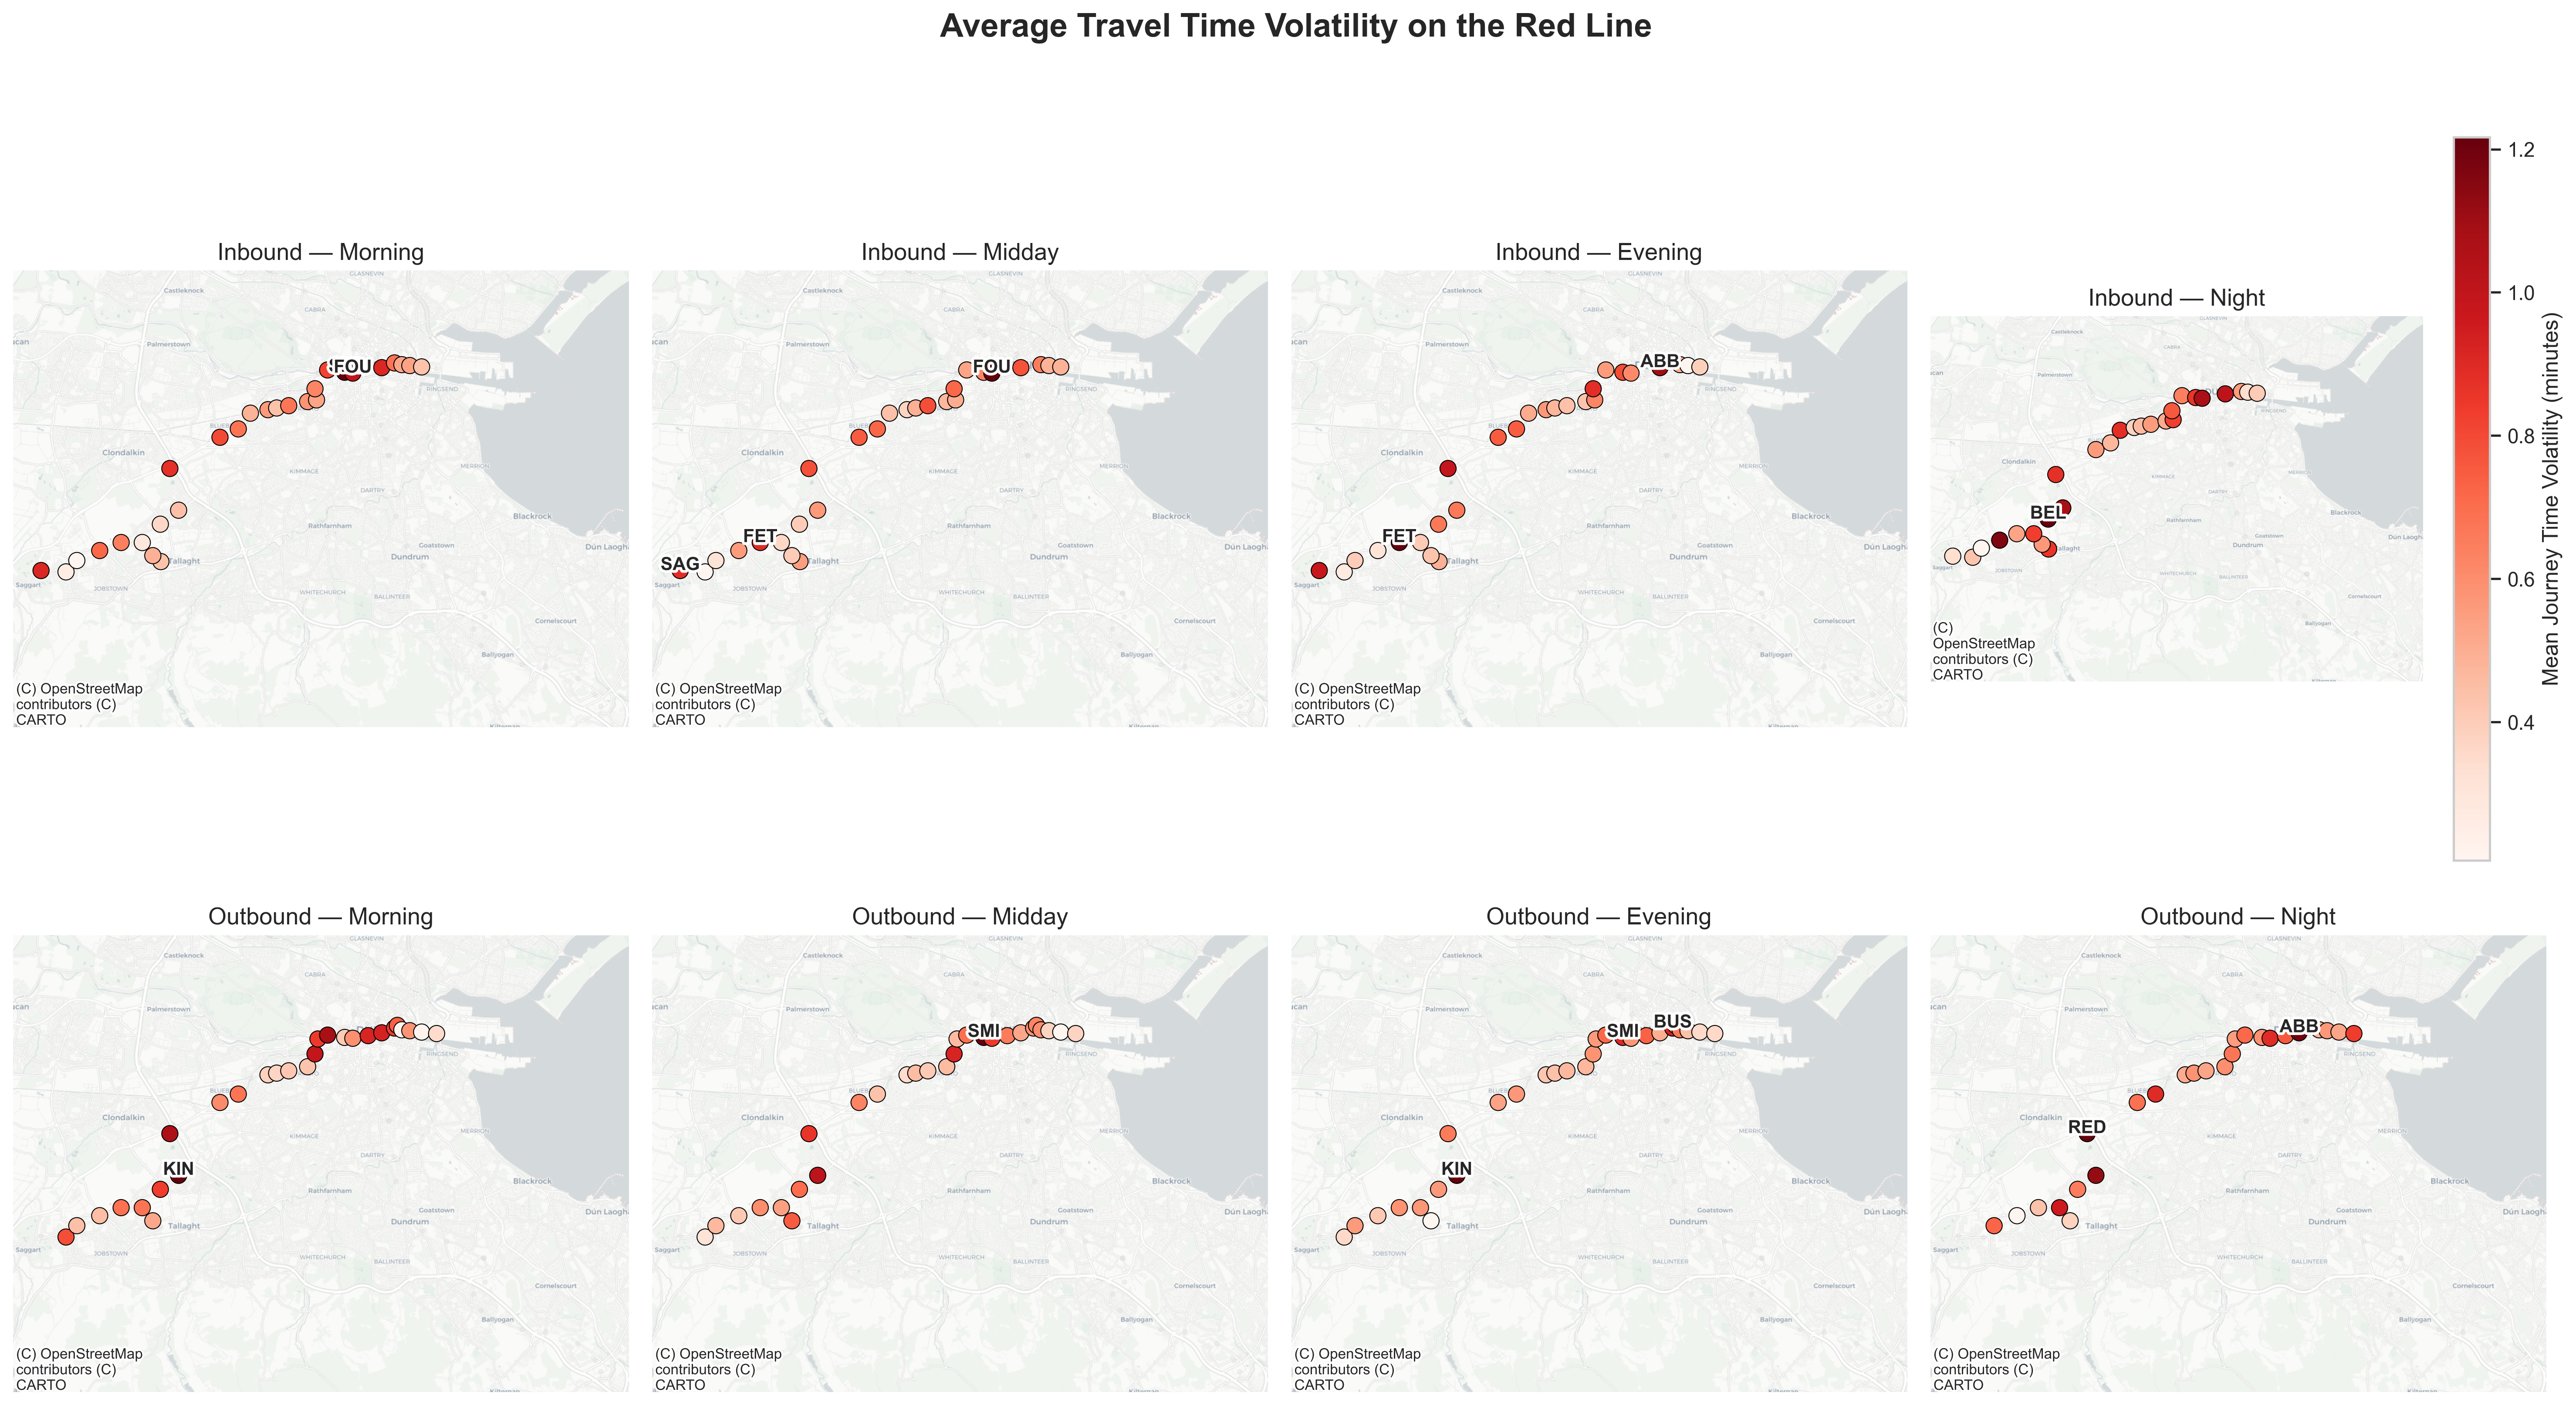
\includegraphics[width=0.85\textwidth]{figures/appendix_figures/travel_time_volatility/volatility_allperiods_red_combined_recovery.png}
  \caption{Recovery}
\end{figure}

\vspace{5cm}
\begin{figure}[H]
  \centering
  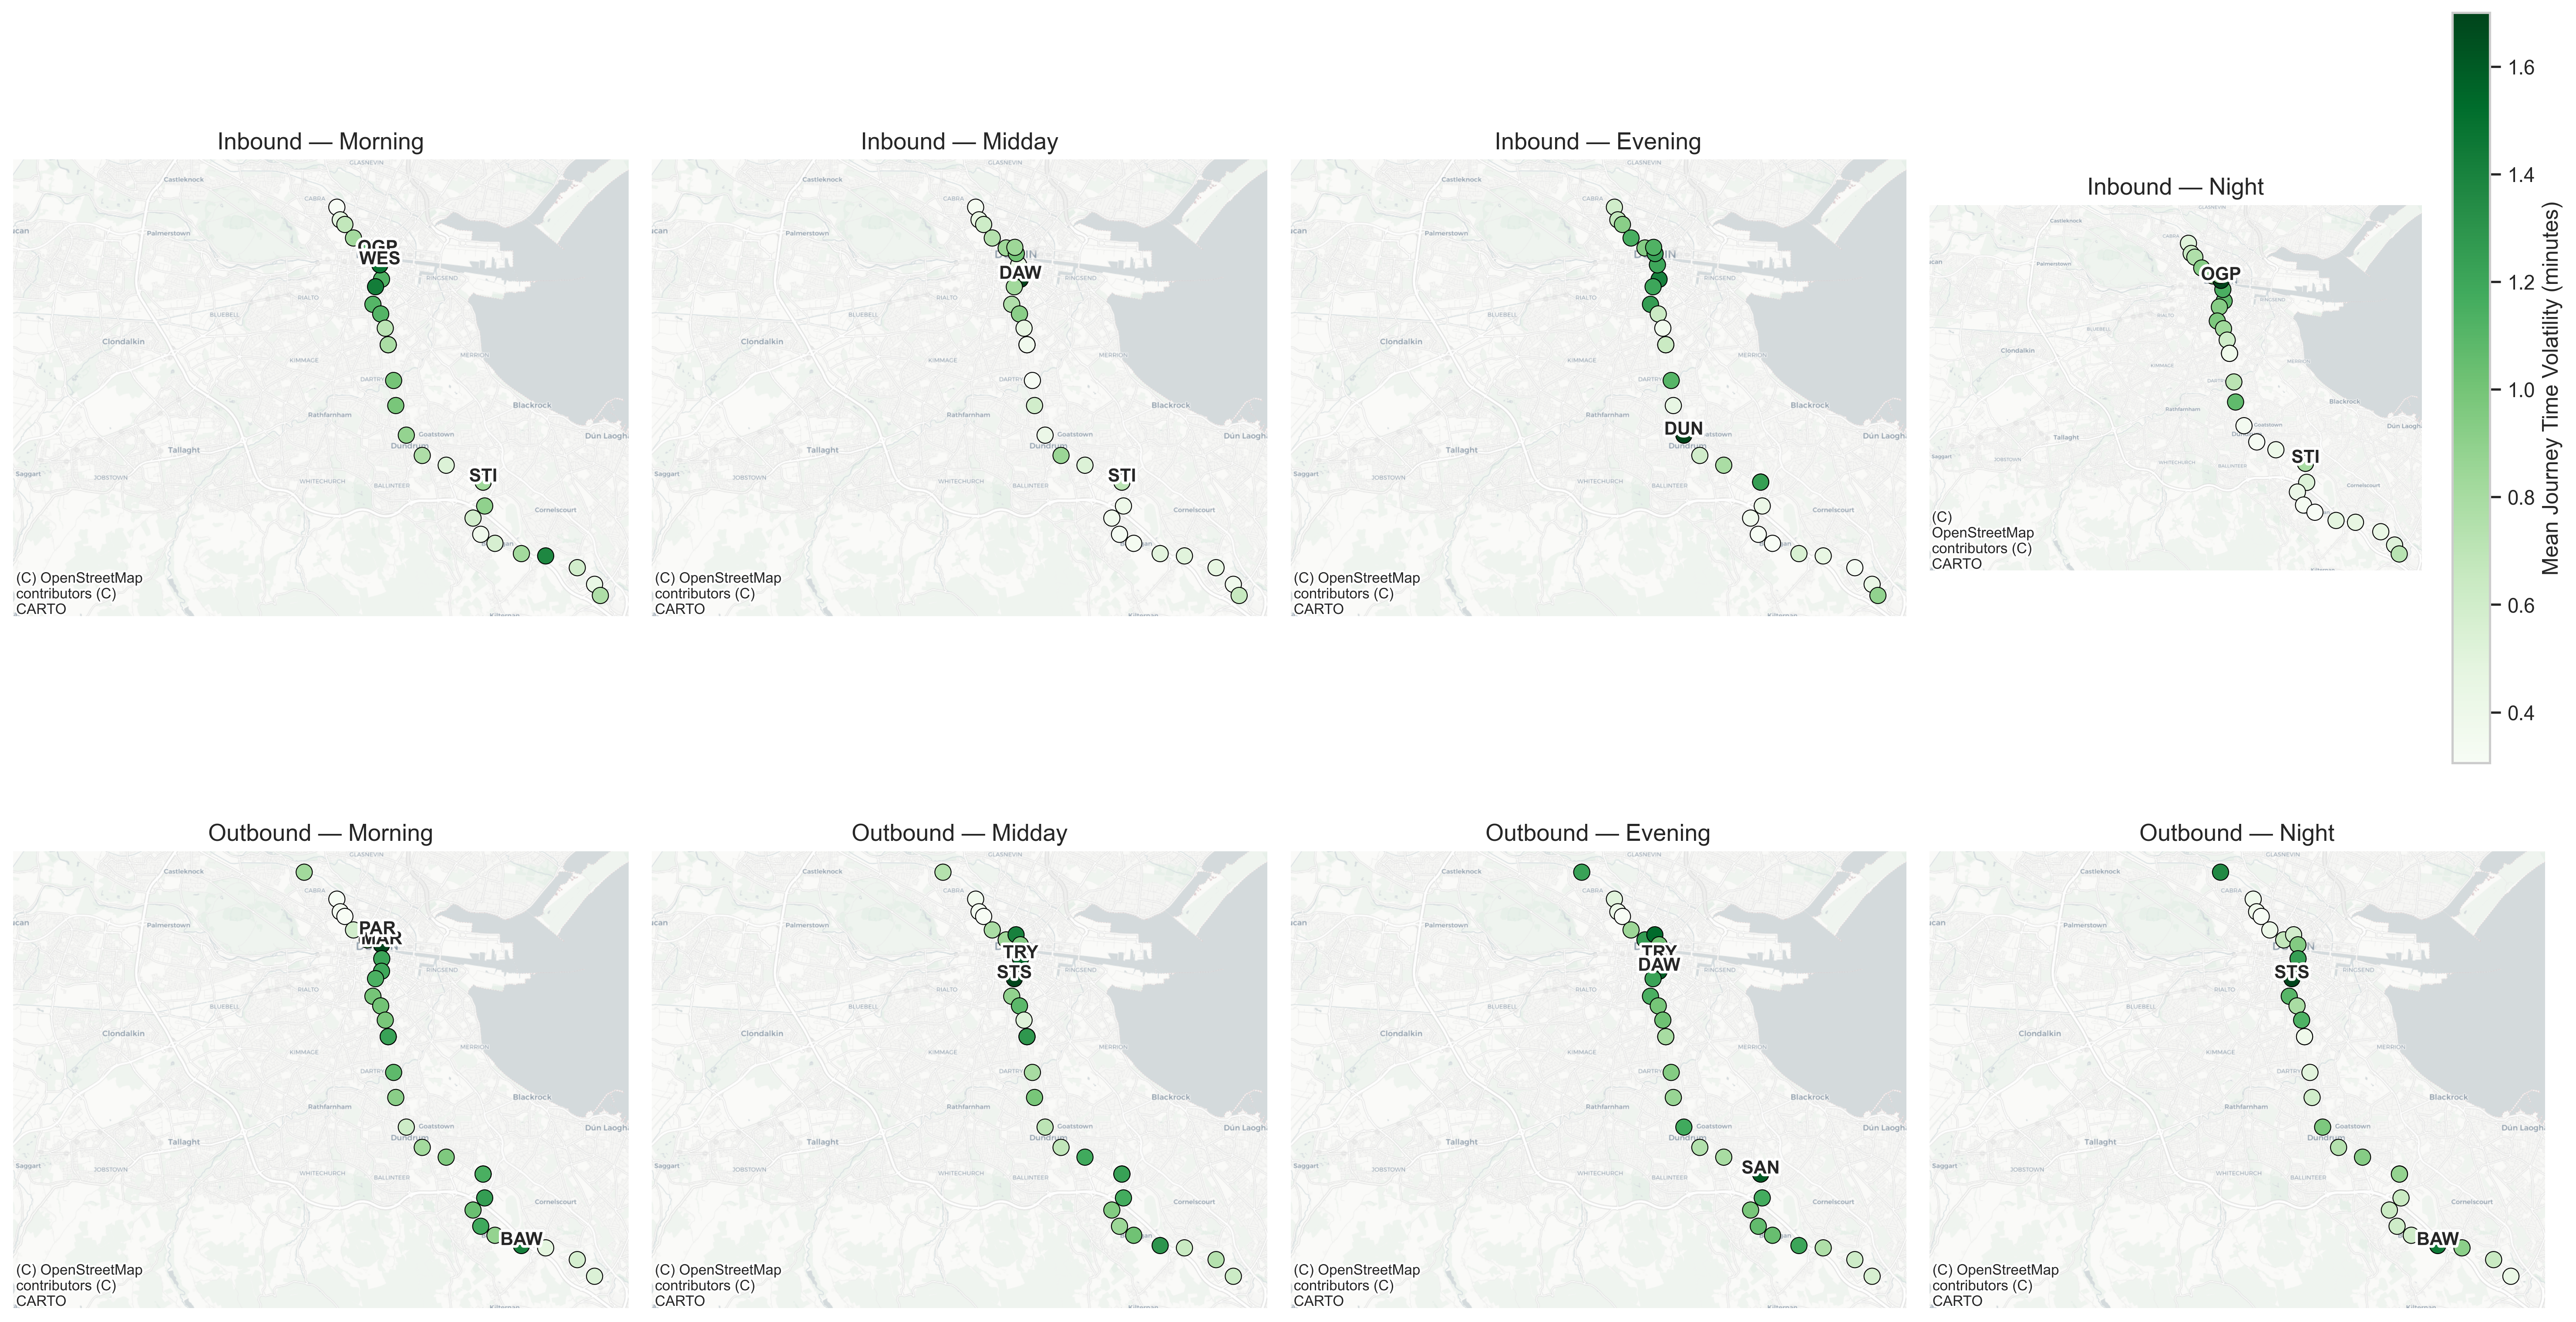
\includegraphics[width=0.85\textwidth]{figures/appendix_figures/travel_time_volatility/volatility_allperiods_green_combined_postcovid.png}
  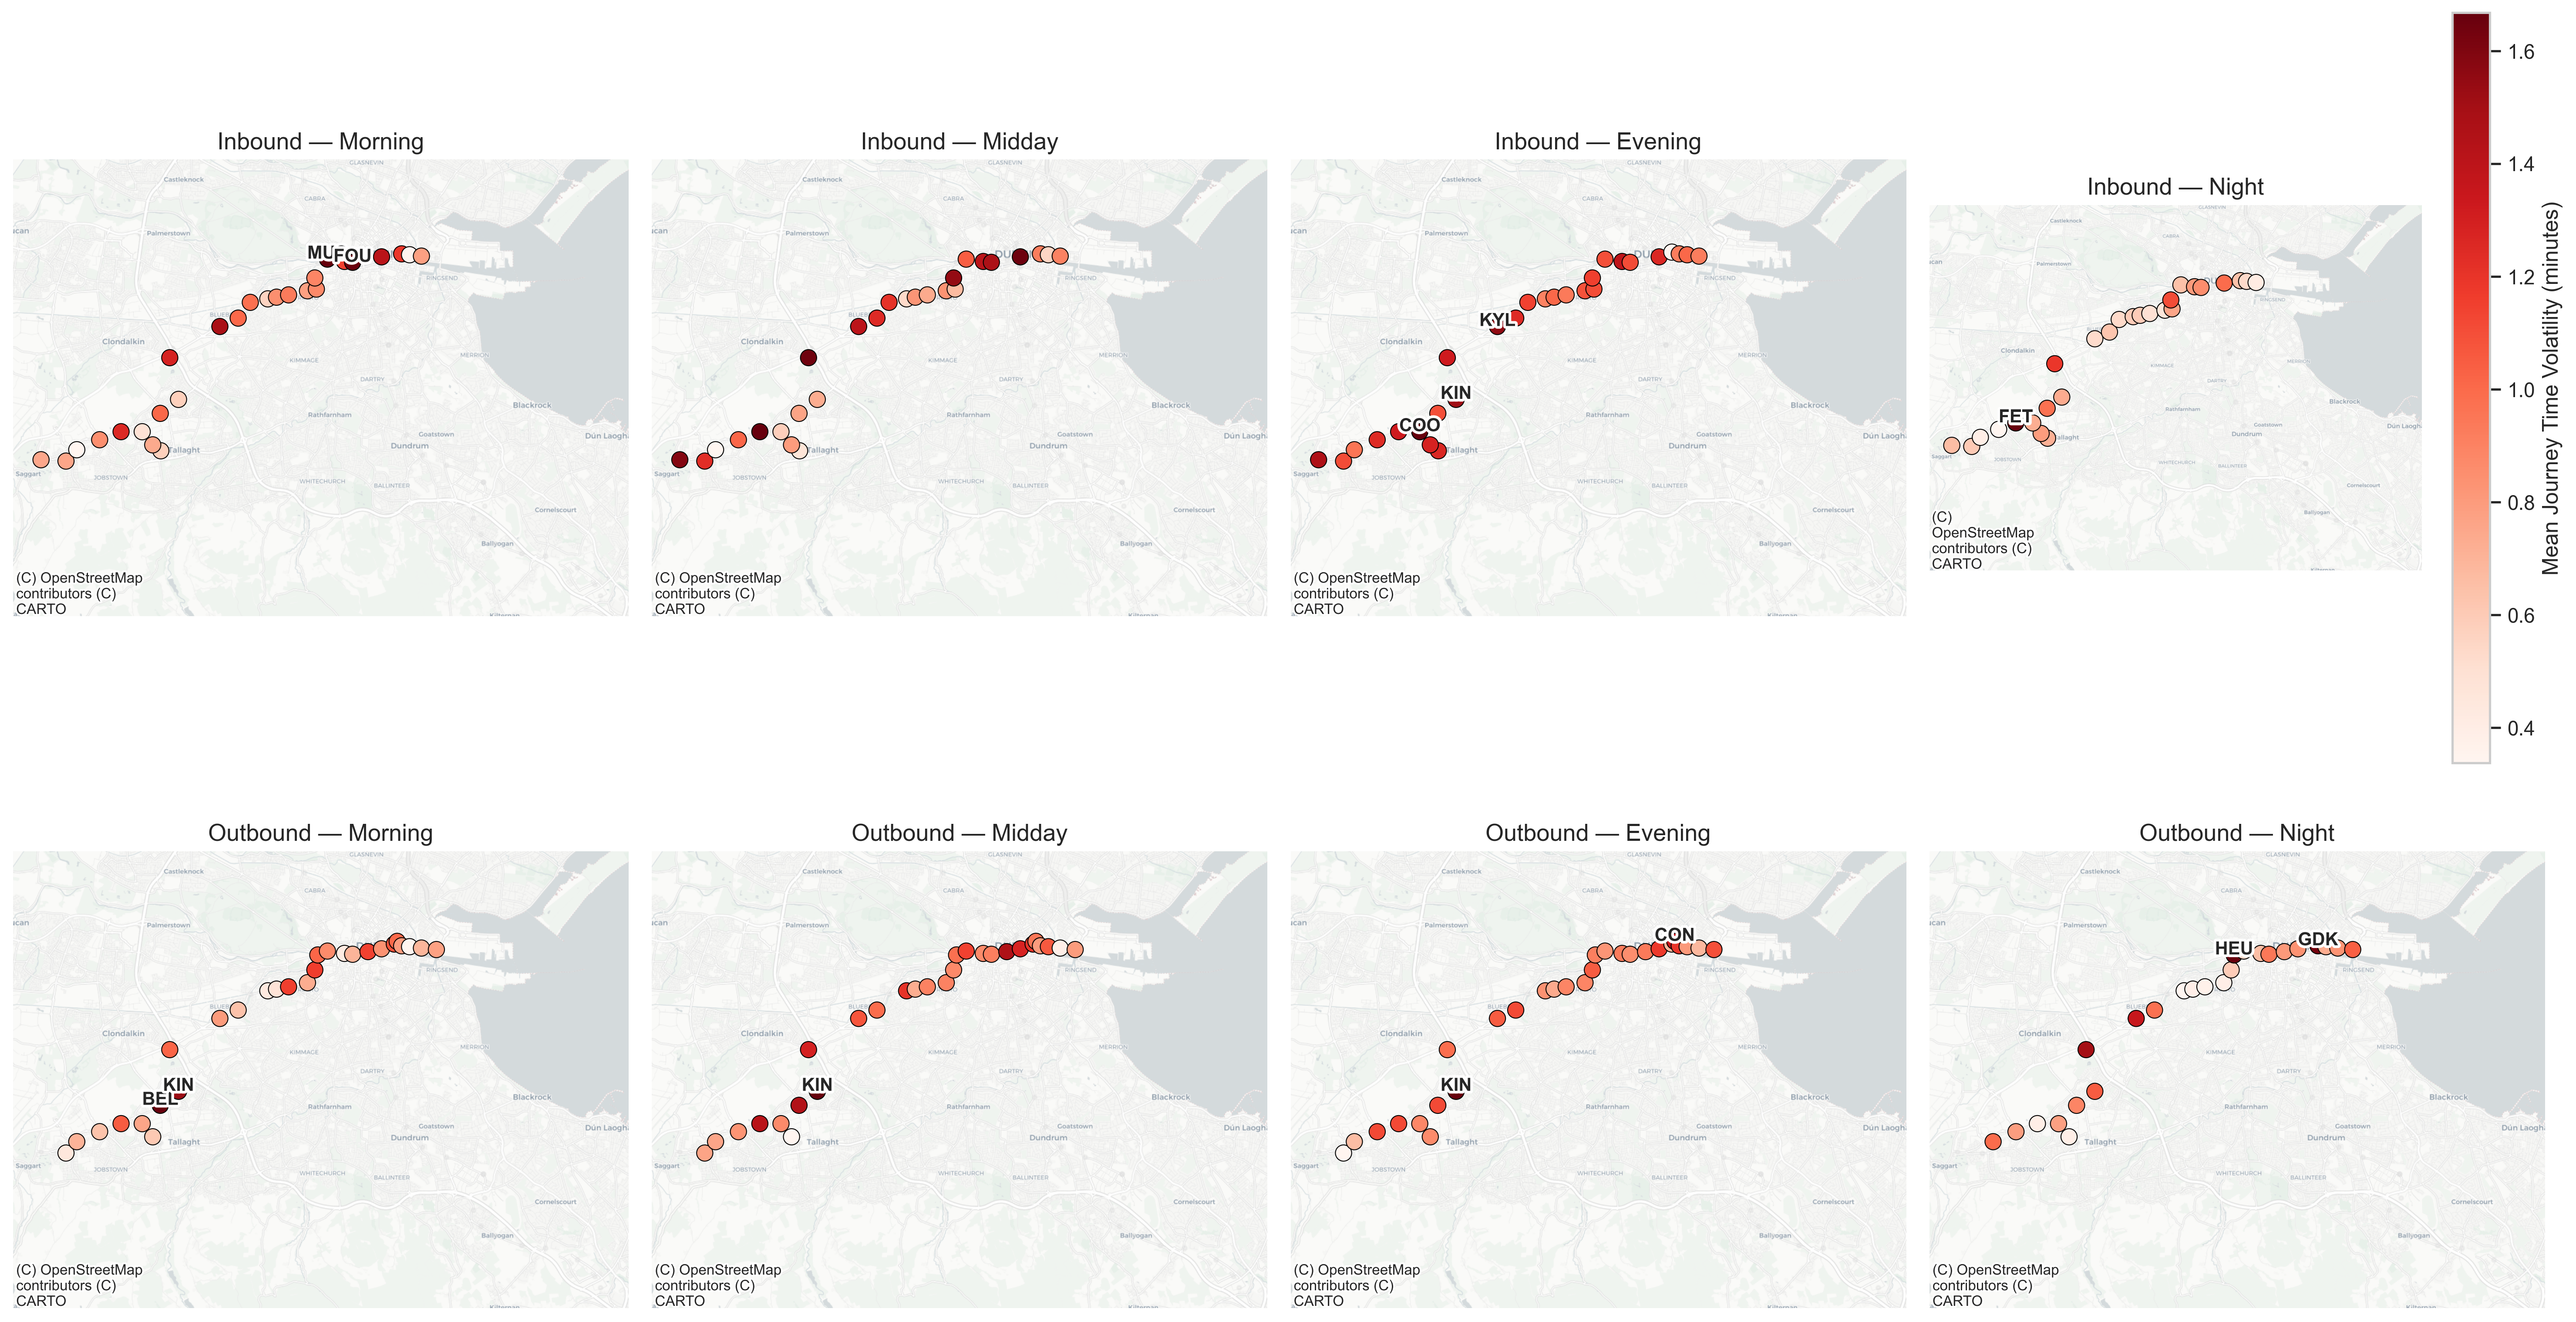
\includegraphics[width=0.85\textwidth]{figures/appendix_figures/travel_time_volatility/volatility_allperiods_red_combined_postcovid.png}
  \caption{Post-COVID}
\end{figure}

% --------------------------------------------------
\newpage
\subsection*{Journey Duration}

\subsubsection*{Duration Across Varied Groups}

\begin{table}[H]
  \centering
  \caption{Average journey durations by phase and line}
  \label{tab:duration_by_phase}
  \begin{tabular}{lcc}
    \textbf{Period} & \textbf{Green Line (min)} & \textbf{Red Line (min)} \\
    Pre-COVID & 50.2 & 48.5 \\
    Lockdown  & 49.8 & 48.2 \\
    Recovery  & 50.2 & 48.9 \\
    Post-COVID & 50.8 & 49.2 \\
  \end{tabular}
\end{table}

\begin{table}[H]
  \centering
  \caption{Time-of-day journey durations }
  \label{tab:duration_by_time}
  \begin{tabular}{lcccc}
    \textbf{Period} & \textbf{Line} & \textbf{Morning} & \textbf{Evening} & \textbf{Night} \\
    Pre-COVID & Green & 49.7 & 47.8 & 55.8 \\
              & Red   & 48.4 & 49.1 & 47.4 \\
    Lockdown  & Green & 49.6 & 47.4 & 55.2 \\
              & Red   & 48.1 & 48.5 & 47.3 \\
    Recovery  & Green & 49.9 & 48.3 & 55.0 \\
              & Red   & 48.8 & 49.2 & 47.8 \\
    Post-COVID & Green & 50.4 & 48.5 & 56.3 \\
              & Red   & 49.0 & 49.7 & 48.3 \\
  \end{tabular}
\end{table}

\subsubsection*{Journey Duration Figures}

\begin{figure}[H]
  \centering
  \begin{subfigure}[t]{0.49\textwidth}
    \centering
    \includegraphics[width=\textwidth]{figures/appendix_figures/journey_duration/duration_hourly_combined_precovid.png}
    \caption*{By Hour}
  \end{subfigure}
  \hfill
  \begin{subfigure}[t]{0.49\textwidth}
    \centering
    \includegraphics[width=\textwidth]{figures/appendix_figures/journey_duration/duration_period_combined_precovid.png}
    \caption*{By Time-of-Day}
  \end{subfigure}
  \caption{Pre-COVID}
\end{figure}

\begin{figure}[H]
  \centering
  \begin{subfigure}[t]{0.49\textwidth}
    \centering
    \includegraphics[width=\textwidth]{figures/appendix_figures/journey_duration/duration_hourly_combined_lockdown.png}
    \caption*{By Hour}
  \end{subfigure}
  \hfill
  \begin{subfigure}[t]{0.49\textwidth}
    \centering
    \includegraphics[width=\textwidth]{figures/appendix_figures/journey_duration/duration_period_combined_lockdown.png}
    \caption*{By Time-of-Day}
  \end{subfigure}
  \caption{Lockdown}
\end{figure}

\begin{figure}[H]
  \centering
  \begin{subfigure}[t]{0.49\textwidth}
    \centering
    \includegraphics[width=\textwidth]{figures/appendix_figures/journey_duration/duration_hourly_combined_recovery.png}
    \caption*{By Hour}
  \end{subfigure}
  \hfill
  \begin{subfigure}[t]{0.49\textwidth}
    \centering
    \includegraphics[width=\textwidth]{figures/appendix_figures/journey_duration/duration_period_combined_recovery.png}
    \caption*{By Time-of-Day}
  \end{subfigure}
  \caption{Recovery}
\end{figure}

\begin{figure}[H]
  \centering
  \begin{subfigure}[t]{0.49\textwidth}
    \centering
    \includegraphics[width=\textwidth]{figures/appendix_figures/journey_duration/duration_hourly_combined_postcovid.png}
    \caption*{By Hour}
  \end{subfigure}
  \hfill
  \begin{subfigure}[t]{0.49\textwidth}
    \centering
    \includegraphics[width=\textwidth]{figures/appendix_figures/journey_duration/duration_period_combined_postcovid.png}
    \caption*{By Time-of-Day}
  \end{subfigure}
  \caption{Post-COVID}
\end{figure}


% --- BIBLIOGRAPHY ---
\clearpage
\addcontentsline{toc}{section}{Bibliography}
\nocite{*}
\begingroup
\sloppy
\printbibliography
\endgroup


\end{document}
